%CASOS DE USO:
%1. Calcular promedio de energía sensada diariamente SAM
%2. Calcular promedio de energía sensada bimestralmente SAM
%3. Enviar muestras del sensor al microcontrolador en tiempo real GIS
%4. Enviar muestras del microcontrolador al servidor. GIS
%5. Enviar muestras del servidor a la aplicacion. ANDRES
%6. Ver reporte bimestral(usuario) ANDRES
%7. Ver monitoreo en tiempo real(usuario) SAM
%8. Emparejar dispositivo(usuario) SAM
%9. Ver menú(usuario) GIS 
%10. Ver notificaciones(usuario) GIS
%11. Monitorear S. Fotovoltaico (aqui se ocuparían las RN's de crear notificación por promedio diario, sistema dejo de producir energía) ANDRES
%12. Almacenar medición en servidor ANDRES
%13. Almacenar notificaciones manualmente(app usuario) SAM






\section{Software}
\subsection{Diagrama de paquetes}
En la Figura \ref{fig:dcu-general} se muestra el diagrama de paquetes del sistema.
\begin{figure}[H]
	\centering
	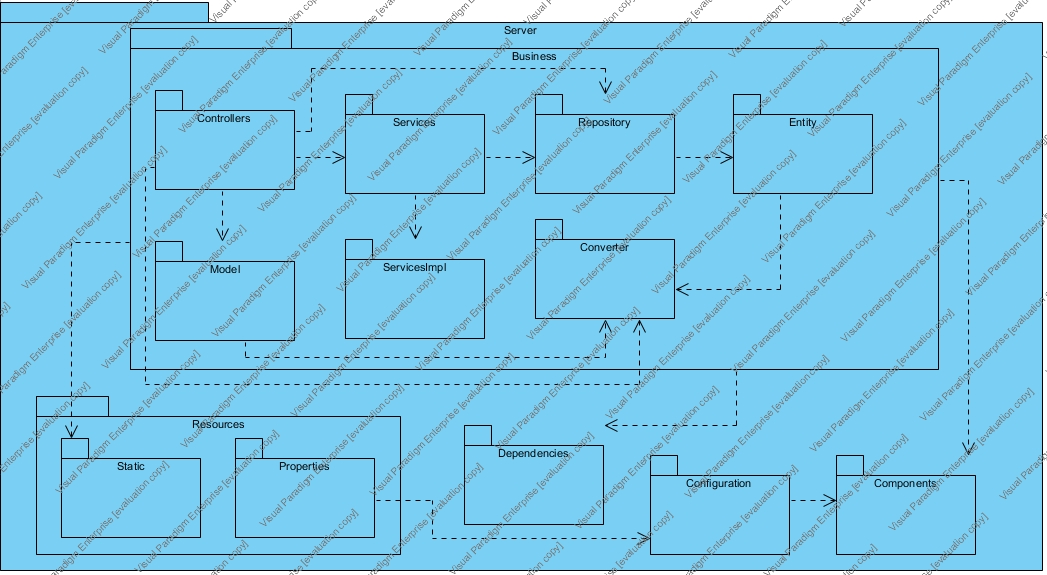
\includegraphics[scale=.198]{Capitulo4/images/Paquetes}
	\caption{Diagrama de paquetes del sistema}
	\label{fig:diagrama_paquetes}
\end{figure}
\subsection{Diagrama de casos de uso general}
En la Figura \ref{fig:dcu-general} se muestra el diagrama general de casos de uso de todo el sistema.
\begin{figure}[H]
	\centering
	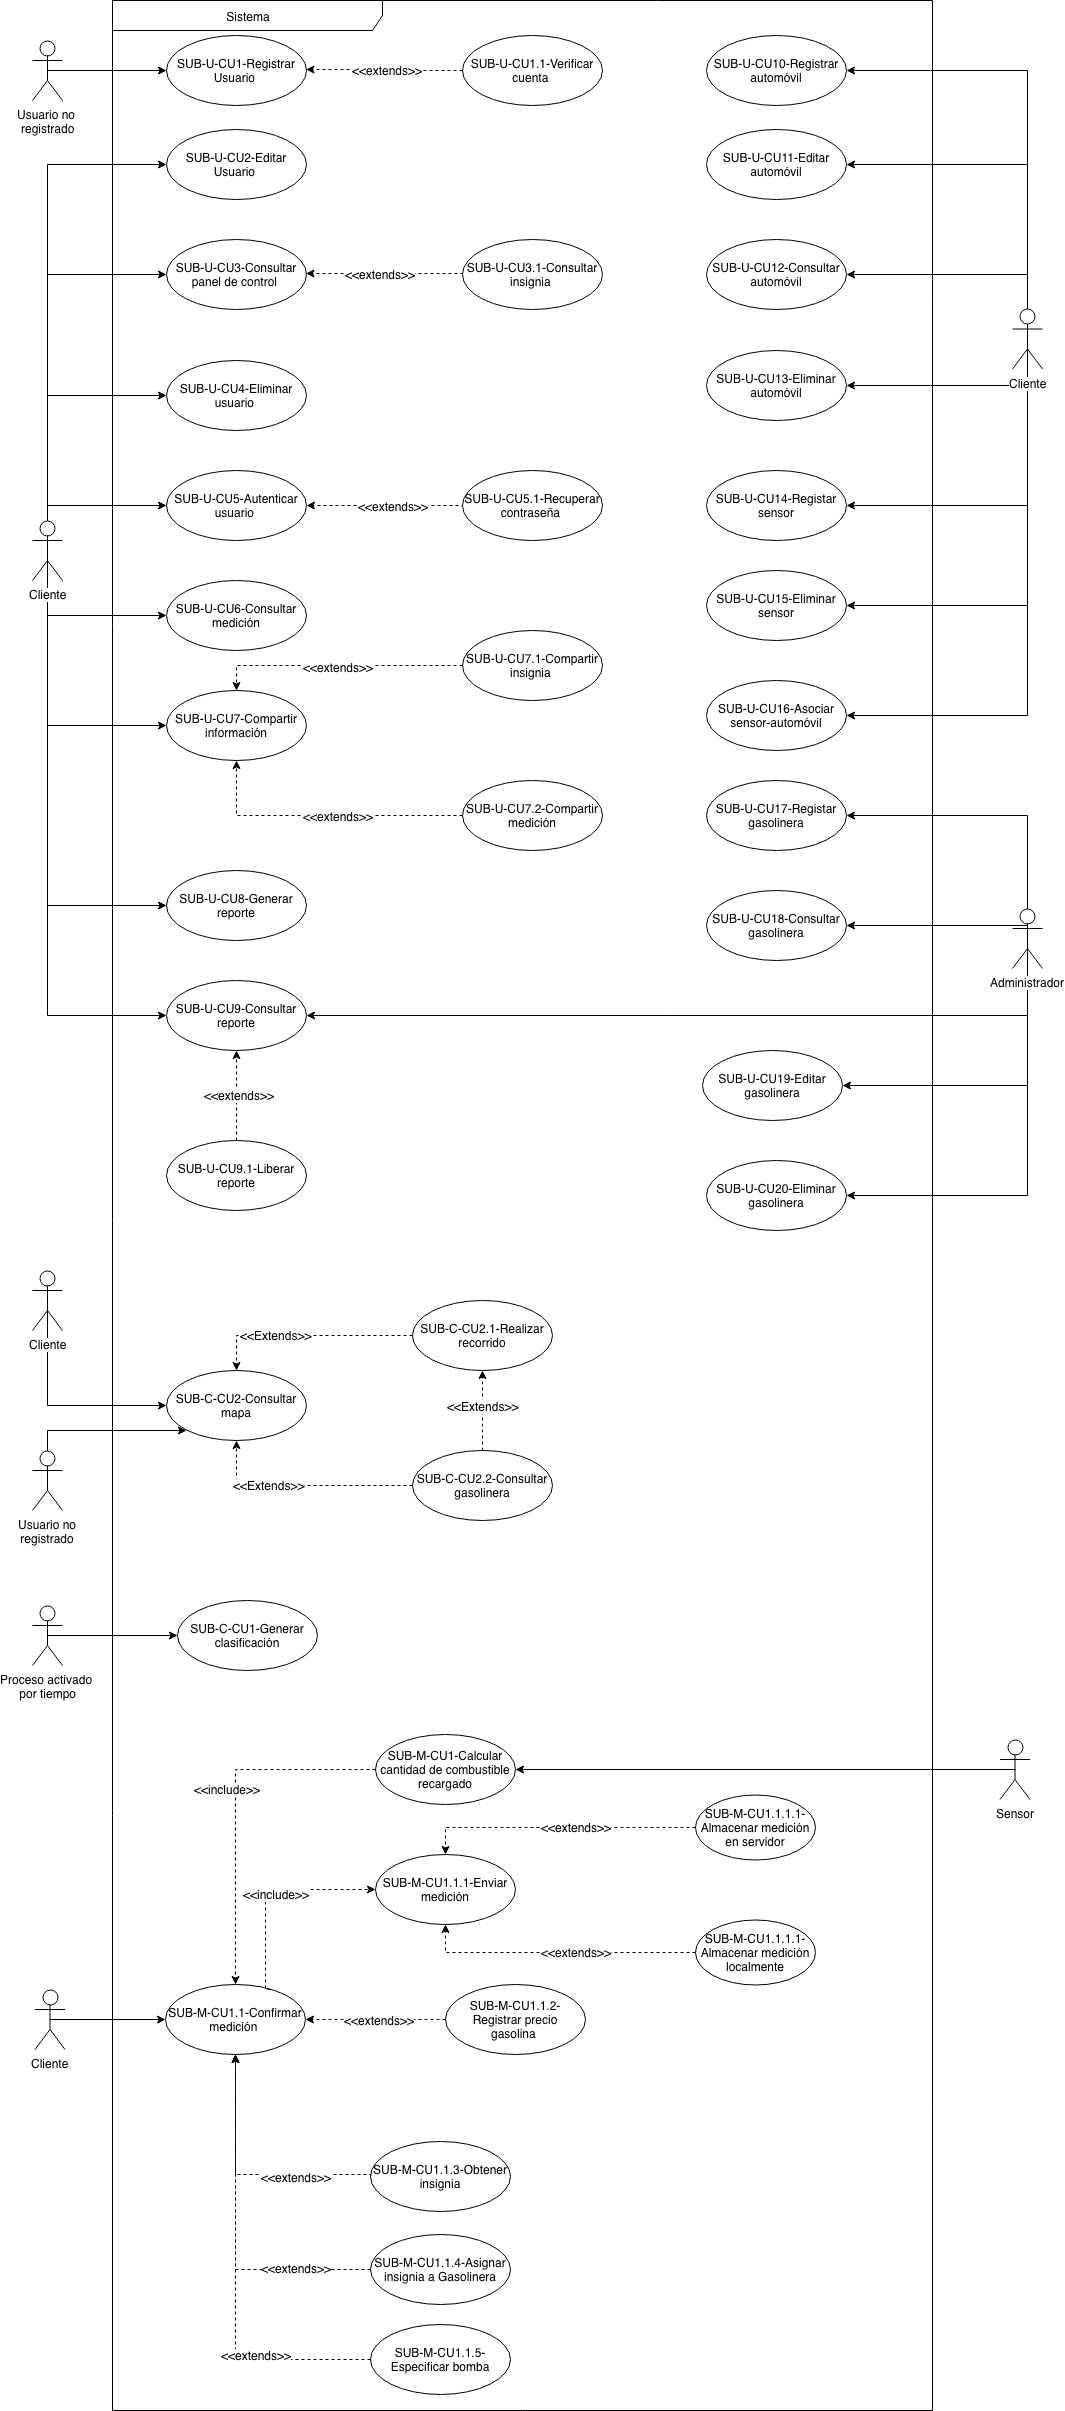
\includegraphics[scale=.198]{Capitulo4/software/submodulos/images/dcu}
	\caption{Diagrama de casos de uso general}
	\label{fig:dcu-general}
\end{figure}
\subsection{Submódulo Sistema de monitoreo}
En esta sección se mostrarán y detallarán los casos de uso que pertenecen al Submódulo del Sistema de monitoreo.
\subsubsection{Diagrama de casos de uso}
En la Figura \ref{fig:dcu-moduloMonitoreo} se observa el diagrama de casos de uso del submódulo del Sistema de monitoreo.
\begin{figure}[H]
	\centering
	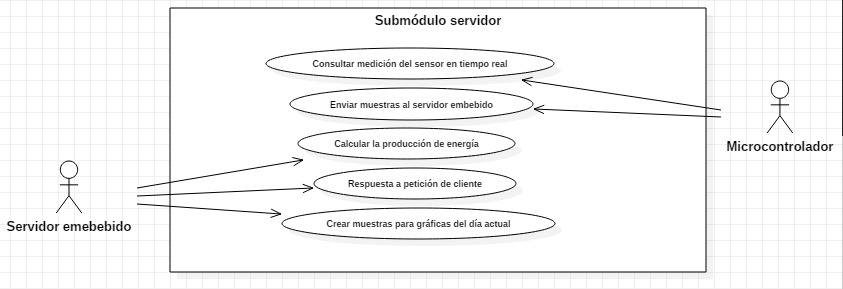
\includegraphics[scale=.6]{Capitulo4/software/submodulos/images/dcuservidor.jpg}
	\caption{Diagrama de casos de uso del submódulo Sistema de monitoreo}
	\label{fig:dcu-moduloMonitoreo}
\end{figure}

%Dudas para revisión:
%   *Condiciones de término
%   *Errores checar si los 3 son correctos
%   *Trayectoria principal
% Agregar regla de negocio de IIC Time Out and Clock Stretching? Si se agrega, incluir la RN en la tabla
\subsubsection{SUB-M-CU1.1-Consultar medición del sensor en tiempo real}\label{SUB-M-CU1.1}
El microcontrolador consulta la medición del sensor MCP39F521 de acuerdo a la Regla de Negocio \ref{RN1} Dichas mediciones son enviadas al microcontrolador por medio del protocolo IIC.
\begin{longtable}{|J{5cm}|J{10.3cm}|}
	\hline
	\textbf{Nombre del caso de uso} &
		SUB-M-CU1.1-Consultar medición del sensor en tiempo real \\ \hline
	\textbf{Objetivo} &
		Enviar las mediciones obtenidas por el sensor hacia el microcontrolador por medio del protocolo IIC, para que éstas puedan ser procesadas por el sistema embebido. \\ \hline
	\textbf{Actores} &
	    \begin{itemize}
		    \item Microcontrolador
		    \item Sensor
		\end{itemize}\\ \hline 
	\textbf{Disparador} & 
		El sensor recibe por medio del protocolo IIC, una trama que contiene la instrucción de lectura solicitada por el microcontrolador, para obtener los valores de la medición realizada por el sensor. \\ \hline 
	\textbf{Entradas} & 
		\begin{itemize}
				\item {[Microcontrolador]} Trama que contiene la instrucción de lectura de medición del sensor.
		\end{itemize}\\ \hline 
	\textbf{Salidas} & 
	    \begin{itemize}
	        \item {[Sensor]} Trama de respuesta de lectura de medición del sensor.
	    \end{itemize}\\ \hline
	\textbf{Precondiciones} & 
		Ninguna \\ \hline
	\textbf{Postcondiciones} &
		\begin{itemize}
			\item La trama de respuesta que contiene la información de la medición obtenida es recibida por el microcontrolador.
		\end{itemize} \\ \hline
	\textbf{Condiciones de término} & 
		\begin{itemize}
		    \item El microcontrolador valida la trama de respuesta enviada por el sensor.
			%DUDA:\item El sensor recibe la trama de acuse de recibido por el microcontrolador.
		\end{itemize} 
		\\ \hline 
	\textbf{Prioridad} & 
		Alta. \\ \hline
	\textbf{Errores} &
		 \begin{itemize}
		 %DUDA: tiempo establecido por I2C Time Out and Clock Stretching?
		 	\item \label{SUB-M-CU1.1:Error1} Error 1: La trama de lectura de medición del sensor no es válida.
		 	\item \label{SUB-M-CU1.1:Error2} Error 2: La trama de respuesta del sensor no fue recibida por el microcontrolador.
		 	\item \label{SUB-M-CU1.1:Error3} Error 3: La trama de respuesta de medición del sensor no es válida.
		 \end{itemize} \\ \hline
	\textbf{Reglas de negocio} & 
	    \begin{itemize}
	      \item  \ref{RN1}
		 \end{itemize}\\ \hline
	% \caption{}
	%\label{desc:SUB-M-CU1}
\end{longtable}

\paragraph{Trayectoria principal}
\label{SUB-M-CU1.1:TP}
	\begin{enumerate}
	    \item {[Microcontrolador]} Envía una trama que contiene la instrucción de lectura de medición del sensor que se desea por medio del protocolo IIC.
	    \item {[Sensor]} Recibe la trama.
	    \item {[Sensor]} Valida que la trama sea correcta. \hyperref[SUB-M-CU1.1:TA]{[Trayectoria Alternativa A]} %Error1
		\item {[Sensor]} Envía la trama de respuesta de medición al microcontrolador por medio del protocolo de comunicación IIC.
		\item {[Microcontrolador]} Recibe la trama de respuesta de lectura de medición que solicitó al sensor.\hyperref[SUB-M-CU1.1:TB]{[Trayectoria Alternativa B]} %Error2
		\item {[Microcontrolador]} Valida que la trama sea correcta por medio del acuse del sensor. \hyperref[SUB-M-CU1.1:TC]{[Trayectoria Alternativa C]}%Error3 
		\item {[Microcontrolador]} Retorna al primer paso de \hyperref[SUB-M-CU1.1:TP]{[Trayectoria Principal]}
	\end{enumerate}
	Fin del caso de uso.

%TA? El sensor recibe una trama de no acuse de recibo por el microcontrolador. \hyperref[SUB-M-CU1.1:TP]{[Trayectoria Principal]}
\paragraph{Trayectoria alternativa A} \label{SUB-M-CU1.1:TA}
	La trama que contiene la instrucción de lectura de medición del sensor no es válida.
	\begin{enumerate}[label=A\arabic*.]
		\item {[Sensor]} Envía una trama para notificar el error al microcontrolador.  
	\end{enumerate}
	Fin de la trayectoria alternativa y retorno al último paso de \hyperref[SUB-M-CU1.1:TP]{[Trayectoria Principal]}  

\paragraph{Trayectoria alternativa B} \label{SUB-M-CU1.1:TB}
	La trama de respuesta de lectura de medición del sensor no fue recibida por el microcontrolador.
	\begin{enumerate}[label=B\arabic*.]
		\item {[Microcontrolador]} Reenvía una trama que contiene la instrucción de lectura de medición del sensor por medio del protocolo IIC.  
	\end{enumerate}
	Fin de la trayectoria alternativa. Regresa al paso 2 de \hyperref[SUB-M-CU1.1:TP]{[Trayectoria Principal]}  
	
\paragraph{Trayectoria alternativa C} \label{SUB-M-CU1.1:TC}
	La trama de respuesta de medición del sensor no es válida.
	\begin{enumerate}[label=C\arabic*.]
		\item {[Sensor]} Genera un código de error.
	\end{enumerate}
	Fin de la trayectoria alternativa y retorno al último paso de \hyperref[SUB-M-CU1.1:TP]{[Trayectoria Principal]} 
%ESTE LO TENGO QUE MODIFICAR
\subsubsection{SUB-M-CU1.2-Calcular promedio bimestral de energía sensada }\label{SUB-M-CU1.2}
El  promedio  de  energía  bimestral es calculado  tomando en cuenta las especificaciones de la Regla de Negocio \ref{RN4} para el cálculo bimestral, este cálculo se realiza con los promedios diarios calculados en los días que abarca el periodo especificado, cuando alguno de estos
periodos culmina y el promedio de energía sensada diariamente del día en curso ha sido calculado como se especifica en el caso de uso \hyperref[SUB-M-CU1.1]{SUB-M-CU1.1}.


\begin{longtable}{|J{5cm}|J{10.3cm}|}
	\hline
	\textbf{Nombre del caso de uso} &
		SUB-M-CU1.2 - Calcular promedio bimestral de energía sensada
 \\ \hline
	\textbf{Objetivo} &
		Obtener la media bimestral de los promedios  diarios de muestras tomadas durante los periodos especificados en la regla de negocios  \ref{RN4} para el cálculo bimestral, y posteriormente ser almacenado.
 \\ \hline
	\textbf{Actores} &
		Servidor embebido \\ \hline 
	\textbf{Disparador} & 
		La ́ultima muestra del día fue tomada, el periodo de toma de muestras especificado en la Regla de Negocio \ref{RN6} ha culminado y el día en curso es el día que marcan el final de uno de los periodos especificados en la regla de negocios \ref{RN4} para el cálculo bimestral. \\ \hline 
	\textbf{Entradas} & 
		\begin{itemize}
				\item Promedios diarios comprendido dentro del periodo que se va a calcular.
		\end{itemize}\\ \hline 
	\textbf{Salidas} & 
		\begin{itemize}
			\item Promedio bimestral de muestras sensadas por el sistema fotovoltaico.
			\item Fecha del día actual en la que se realiza el cálculo.
		\end{itemize} \\ \hline
	\textbf{Precondiciones} &
		Ninguna.\\ \hline
	\textbf{Postcondiciones} &
		\begin{itemize}
			\item El promedio calculado junto con la fecha del día en curso son almacenados.
		\end{itemize}\\ \hline
	\textbf{Condiciones de término} & 
		\begin{itemize}
			\item Se obtiene un número flotante que representa el promedio bimestral de energía que ha sido sensada.
			\item Se obtiene la fecha del día en curso del cual se realiza el promedio.
		\end{itemize} \\ \hline 
	\textbf{Prioridad} & 
		Alta. \\ \hline
	\textbf{Errores} & 
		Ninguno \\ \hline
	\textbf{Reglas de negocio} & 
		\begin{itemize}
			\item \ref{RN4}
			\item \ref{RN6}
		\end{itemize} \\ \hline

	% \caption{}
	%\label{desc:SUB-M-CU1}
\end{longtable}

\paragraph{Trayectoria principal}
	\begin{enumerate}
		\item {[Sensor]} El promedio diario del último día de uno de los periodos especificado en la regla de negocios \ref{RN4} para el cálculo bimestral es calculado como lo indica el caso de uso \hyperref[SUB-M-CU1.1]{SUB-M-CU1.1} y es almacenado.
		\item  {[Sistema]} Consulta de la base de datos los promedios diarios de los días que abarca el periodo en curso, por ejemplo, si el día actual es 30 de Abril, se recuperarán los promedios diarios del 1 de Marzo al 30 de Abril.
		\item {[Sistema]} Realiza el promedio con los promedios diarios consultados.
		\item {[Sistema]} Obtiene la fecha actual
		\item {[Sistema]} Almacena tanto el promedio como la fecha actual.
	\end{enumerate}
	Fin del caso de uso.

%PREGUNTAR A VH

\subsubsection{SUB-M-CU1.3-Enviar mediciones del sensor al microcontrolador en tiempo real}\label{SUB-M-CU1.3}
El dispositivo de monitoreo MCP39F521 se encarga de obtener las mediciones en tiempo real del sistema fotovoltaico; dichas mediciones son enviadas al microcontrolador por medio del protocolo IIC.
\begin{longtable}{|J{5cm}|J{10.3cm}|}
	\hline
	\textbf{Nombre del caso de uso} &
		SUB-M-CU1.3-Enviar mediciones del sensor al microcontrolador en tiempo real \\ \hline
	\textbf{Objetivo} &
		Enviar las mediciones obtenidas por el sensor hacia el microcontrolador por medio del protocolo IIC, para que éstas puedan ser procesadas por el Sistema embebido. \\ \hline
	\textbf{Actores} &
		Sensor \\ \hline 
	\textbf{Disparador} & 
		El sensor obtiene una lectura de medición del sistema fotovoltaico. \\ \hline 
	\textbf{Entradas} & 
		\begin{itemize}
				\item Medición obtenida por el sensor
		\end{itemize}\\ \hline 
	\textbf{Salidas} & Trama generada por el protocolo IIC.
		% \begin{itemize}
		% 	\item Cantidad de gasolina que debió ser cargada al automóvil.
		% \end{itemize} 
		\\ \hline
	\textbf{Precondiciones} & 
		Existe una medición del Sistema fotovoltaico.\\ \hline
	\textbf{Postcondiciones} &
		\begin{itemize}
			\item La trama que contiene la información de la medición obtenida es recibida por el microcontrolador.
		\end{itemize} \\ \hline
	\textbf{Condiciones de término} & 
		\begin{itemize}
			\item El sensor recibe la trama de acuse de recibido por el microcontrolador.
		\end{itemize} 
		\\ \hline 
	\textbf{Prioridad} & 
		Alta. \\ \hline
	\textbf{Errores} & Ninguno.
		 %\begin{itemize}
		 %	\item \label{SUB-M-CU1.3:Error1} Error 1: La información de la medición no pudo ser enviada al microcontrolador.
		 %\end{itemize} 
		\\ \hline
		% \begin{itemize}
	\textbf{Reglas de negocio} & \ref{RN1}
		% 	\item \ref{RN1}.
		% \end{itemize}
		 \\ \hline
	% \caption{}
	%\label{desc:SUB-M-CU1}
\end{longtable}

\paragraph{Trayectoria principal}
\label{SUB-M-CU1.3:TP}
	\begin{enumerate}
		\item {[Sensor]} Recibe como entrada el voltaje y la corriente que proviene del Sistema fotovoltaico.
		\item {[Sensor]} Realiza una conversión Analógica a Digital de la información recibida. 
		\item {[Sensor]} Envía la trama que contiene la información de medición al microcontrolador por medio del protocolo de comunicación IIC.
		\item {[Sensor]} Recibe trama de acuse de recibo por el microcontrolador. \hyperref[SUB-M-CU1.3:TA]{[Trayectoria Alternativa A]}
	\end{enumerate}
	Fin del caso de uso.

\paragraph{Trayectoria alternativa A} \label{SUB-M-CU1.3:TA}
	El sensor recibe una trama de no acuse de recibo por el microcontrolador.
	\begin{enumerate}[label=A\arabic*.]
		\item {[Sensor]} Regresa al punto 3 de \hyperref[SUB-M-CU1.3:TP]{[Trayectoria Principal]}  
	\end{enumerate}
	Fin de la trayectoria.

%Dudas:
%   *Condición de término
%   *Trayectoria Principal
%   *Checar los errores
\subsubsection{SUB-M-CU1.4-Enviar muestras al Servidor embebido}\label{SUB-M-CU1.4}
El microcontrolador DSPIC30F4013 envía las muestras obtenidas del Sistema fotovoltaico a través del módulo WiFi como se especifica en las Reglas de Negocios \ref{RN2} y \ref{RN17} al Servidor embebido.
\begin{longtable}{|J{5cm}|J{10.3cm}|}
	\hline
	\textbf{Nombre del caso de uso} &
		SUB-M-CU1.4-Enviar muestras al Servidor embebido \\ \hline
	\textbf{Objetivo} &
		Enviar las muestras obtenidas por el microcontrolador al Servidor embebido para su posterior procesamiento. \\ \hline
	\textbf{Actores} &
	    \begin{itemize}
		    \item Microcontrolador
		    \item Servidor embebido
		\end{itemize}\\ \hline 
	\textbf{Disparador} & 
		Conexión establecida entre nodo sensor y microcontrolador.\\ \hline
	\textbf{Entradas} & %Ninguna
		\begin{itemize}%especificar
				\item Muestra obtenida del Sistema fotovoltaico.
		\end{itemize}
		\\ \hline 
	\textbf{Salidas} & 
	    \begin{itemize}%Paquete TCP
	        \item Paquete TCP.
	    \end{itemize}\\ \hline
	\textbf{Precondiciones} & 
		\begin{itemize}
		    \item El periodo de toma de muestras especificado en la Regla de Negocios \ref{RN6} no ha culminado.
		\end{itemize}\\ \hline
	\textbf{Postcondiciones} &
		\begin{itemize}
			\item El paquete TCP es recibido por el Servidor embebido.
		\end{itemize} \\ \hline
	\textbf{Condiciones de término} & 
		\begin{itemize}
		    \item El Servidor embebido envía trama de acuse de recibo al módulo WiFi del microcontrolador.%preguntar por trama tcp del lado del servidor
		\end{itemize} 
		\\ \hline 
	\textbf{Prioridad} & 
		Alta. \\ \hline
	\textbf{Errores} &%No hay conexion con el servidor o la red, 
		 \begin{itemize}
		 	\item \label{SUB-M-CU1.4:Error1} Error 1: El servidor envía una trama de no acuse de recibo al módulo WiFi.
		 	%\item \label{SUB-M-CU1.3:Error2} Error 2: La trama de respuesta de lectura de medición del sensor no fue recibida por el microcontrolador en el tiempo establecido.
		 	%\item \label{SUB-M-CU1.3:Error3} Error 3: El checksum de la trama de respuesta de lectura de medición del sensor no es válido.
		 \end{itemize} \\ 
		 \hline
	\textbf{Reglas de negocio} & 
	    \begin{itemize}
	      \item  \ref{RN2}
	      \item  \ref{RN6}
		 \end{itemize}%\\ \hline
		 \hline
	% \caption{}
	%\label{desc:SUB-M-CU1}
\end{longtable}

\paragraph{Trayectoria principal}
\label{SUB-M-CU1.4:TP}
	\begin{enumerate}
	    \item {[Microcontrolador]} Envía la muestra de medición por medio de la interfaz UART al módulo WiFi del microcontrolador.
	    \item {[Módulo WiFi Microcontrolador]} Recibe la muestra de medición por medio de la interfaz UART.
	    \item {[Módulo WiFi Microcontrolador]} Envía la trama con la información de la muestra a través del protocolo TCP al módulo WiFi del Servidor embebido.
	    \item {[Módulo WiFi Servidor Embebido]} Recibe la trama con la información de la muestra a través del protocolo TCP.\hyperref[SUB-M-CU1.4:TA]{[Trayectoria Alternativa A]}
	    \item {[Módulo WiFi Servidor embebido]} Valida que la trama sea correcta. 
	    \item {[Módulo WiFi Servidor embebido]} Envía trama de acuse de recibo al módulo WiFi del microcontrolador por medio del protocolo TCP. \hyperref[SUB-M-CU1.4:TB]{[Trayectoria Alternativa B]}
	    \item {[Módulo WiFi Microcontrolador]} Recibe trama de acuse de recibo del módulo WiFi del Servidor embebido.
	    %?
	\end{enumerate}
	Fin del caso de uso.


\paragraph{Trayectoria alternativa A} \label{SUB-M-CU1.4:TA}
	El módulo WiFi del Servidor Embebido no recibe la trama por lo que no envía acuse de recibo al módulo WiFi del microcontrolador
	\begin{enumerate}[label=A\arabic*.]
		\item {[Módulo WiFi Microcontrolador]} Reenvía la trama con la información de la muestra a través del protocolo TCP al módulo WiFi del Servidor embebido.
		\item {[Módulo WiFi Servidor Embebido]} Continúa en el paso 4 de la \hyperref[SUB-M-CU1.4:TP]{[Trayectoria Principal]}
	\end{enumerate}
	Fin de la trayectoria alternativa.

\paragraph{Trayectoria alternativa B} \label{SUB-M-CU1.4:TB}
	El Módulo WiFi del Servidor embebido envía trama de no acuse de recibo al módulo WiFi del microcontrolador.
	\begin{enumerate}[label=B\arabic*.]
		\item {[Módulo WiFi Servidor embebido]} Envía trama de no acuse de recibo al módulo WiFi del microcontrolador por medio del protocolo TCP.
		\item {[Módulo WiFi Microcontrolador]} Recibe trama de no acuse de recibo del módulo WiFi del Servidor embebido.
		\item {[Módulo WiFi Microcontrolador]} Reenvía la trama con la información de la muestra a través del protocolo TCP al módulo WiFi del Servidor embebido.
		\item {[Módulo WiFi Servidor Embebido]} Continúa en el paso 4 de la \hyperref[SUB-M-CU1.4:TP]{[Trayectoria Principal]}
	\end{enumerate}
	Fin de la trayectoria alternativa.
%Dudas para revisión:
%   *Condiciones de término
%   *Errores checar si los 3 son correctos
%   *Trayectoria principal
% Agregar regla de negocio de IIC Time Out and Clock Stretching? Si se agrega, incluir la RN en la tabla
\subsubsection{SUB-M-CU1.5-Crear muestras para gráficas del día actual}\label{SUB-M-CU1.5}
El servidor consultará el archivo de tiempo real en el tiempo definido en la regla de negocio \ref{RN6}, con el propósito de crear una gráfica que represente la producción de energía a lo largo de un día.
\begin{longtable}{|J{5cm}|J{10.3cm}|}
	\hline
	\textbf{Nombre del caso de uso} &
		SUB-M-CU1.5-Crear gráficas de tiempo real \\ \hline
	\textbf{Objetivo} &
		Guardar las muestras en el tiempo establecido en la regla de negocio \ref{RN6} en un archivo para generar una gráfica de energía en el tiempo. \\ \hline
	\textbf{Actores} &
	    \begin{itemize}
		    \item Servidor Embebido
		\end{itemize}\\ \hline 
	\textbf{Disparador} & 
		Transcurre el tiempo indicado en la regla de negocio \ref{RN6} \\ \hline 
	\textbf{Entradas} & 
		\begin{itemize}
				\item {[Servidor Embebido]} Muestra del archivo de tiempo real
		\end{itemize}\\ \hline 
	\textbf{Salidas} & 
	    \begin{itemize}
	        \item {[Sensor]} Archivo de muestras del día actualizado
	    \end{itemize}\\ \hline
	\textbf{Precondiciones} & 
		Ninguna \\ \hline
	\textbf{Postcondiciones} &
		Ninguna \\ \hline
	\textbf{Condiciones de término} & 
		\begin{itemize}
		    \item {[Servidor Embebido]} Almacenamiento de la muestra obtenida del archivo de tiempo real en archivo de muestras del día.
		\end{itemize} 
		\\ \hline 
	\textbf{Prioridad} & 
		Alta. \\ \hline
	\textbf{Errores} &
		 \begin{itemize}
		 %DUDA: tiempo establecido por I2C Time Out and Clock Stretching?
		 	\item \label{SUB-M-CU1.5:Error1} Error 1: El archivo de tiempo real no existe.
		 	\item \label{SUB-M-CU1.5:Error2} Error 2: El archivo de tiempo real tiene una hora atrasada.
		 \end{itemize} \\ \hline
	\textbf{Reglas de negocio} & 
	    \begin{itemize}
	      \item  \ref{RN6}
		 \end{itemize}\\ \hline
	% \caption{}
	%\label{desc:SUB-M-CU1}
\end{longtable}

\paragraph{Trayectoria principal}
\label{SUB-M-CU1.5:TP}
	\begin{enumerate}
	    \item {[Servidor Embebido]} Transcurre el tiempo establecido en la regla de negocio \ref{RN6}
	    \item {[Servidor Embebido]} Obtiene por cada nodo de cada microcontrolador su valor en tiempo real. \hyperref[SUB-M-CU1.5:TB]{[Trayectoria Alternativa A]} \hyperref[SUB-M-CU1.5:TB]{[Trayectoria Alternativa B]}
	    \item {[Servidor Embebido]} Guarda el valor obtenido en las muestras del día de hoy.
	    \item {[Servidor Embebido]} Espera al término del minuto cuando sea propio.
		\item {[Servidor Embebido]} Retorna al paso 1 de \hyperref[SUB-M-CU1.5:TP]{[Trayectoria Principal]}
	\end{enumerate}
	Fin del caso de uso.

%TA? El sensor recibe una trama de no acuse de recibo por el microcontrolador. \hyperref[SUB-M-CU1.5:TP]{[Trayectoria Principal]}
\paragraph{Trayectoria alternativa A} \label{SUB-M-CU1.5:TA}
	El archivo de tiempo real no existe.
	\begin{enumerate}[label=A\arabic*.]
		\item {[Servidor Embebido]} Guarda como valor de producción en el archivo de tiempo real y de muestras del día -1, que indica error con el servicio del microcontrolador.
	\end{enumerate}
	Fin de la trayectoria alternativa. Regresa al paso 3 de \hyperref[SUB-M-CU1.5:TP]{[Trayectoria Principal]}  

\paragraph{Trayectoria alternativa B} \label{SUB-M-CU1.5:TB}
	El archivo de tiempo real tiene una hora atrasada.
	\begin{enumerate}[label=B\arabic*.]
		\item {[Servidor Embebido]} Guarda como valor de producción en el archivo de tiempo real y de muestras del día -1, que indica error con el servicio del microcontrolador.  
	\end{enumerate}
	Fin de la trayectoria alternativa. Regresa al paso 3 de \hyperref[SUB-M-CU1.5:TP]{[Trayectoria Principal]}  

\newpage
\subsection{Submódulo Usuario}
\subsubsection{Diagrama de casos de uso}
%En la Figura \ref{fig:dcu-usuarios} se observa el diagrama de casos de uso del submódulo.
%\begin{figure}[H]
%	\centering
%	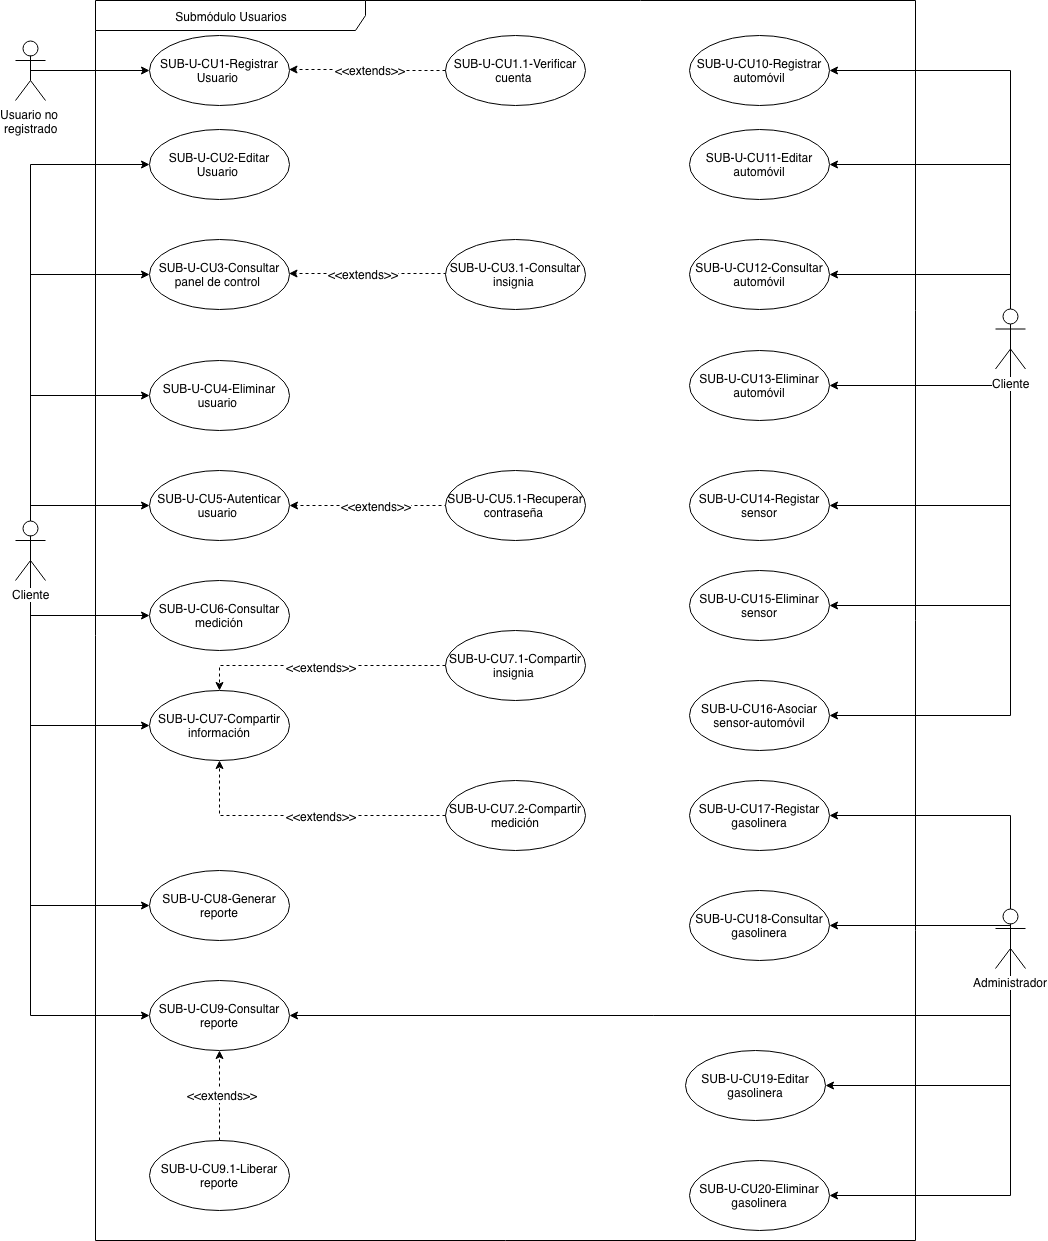
\includegraphics[scale=.4]{Capitulo4/software/submodulos/usuarios/images/dcu}
%	\caption{Diagrama de casos de uso del submódulo Usuarios}
%	\label{fig:dcu-usuarios}
%\end{figure}
%\newpage

\subsubsection{SUB-U-CU1.1-Ver estado de generación actual}\label{SUB-U-CU1.1}
La barra de estado de generación actual se trata de un componente de la interfaz \hyperref[fig:monitoreoReal]{[IU Ver Generación Actual]} y es la encargada de mostrar el estado de generación actual de uno de los nodos que está conectado al servidor, evaluándolo con la Regla de Negocios \ref{RN12}, con actualizaciones en el tiempo establecido en la Regla de Negocios \ref{RN22}, la comunicación con el servidor se logrará mediante el patrón de intercambio de mensajes de la Regla de Negocios \ref{RN8}, con el formato de datos establecido en la Regla de Negocios \ref{RN11}   
\begin{longtable}{|J{5cm}|J{10.3cm}|}
	\hline
	\textbf{Nombre del caso de uso} &
		SUB-U-CU1.1-Ver estado de generación actual \\ \hline
	\textbf{Objetivo} &
		Conseguir la muestra que contiene el valor actual de generación de energía de un nodo y mostrarlo al usuario. \\ \hline
	\textbf{Actores} &
		\begin{itemize}
		    \item Usuario
			\item Servidor embebido
			\item Aplicación móvil
		\end{itemize} \\ \hline
	\textbf{Disparador} & 
	    El usuario inicia la aplicación desde su dispositivo móvil.\\ \hline 
	\textbf{Entradas} & 
		\begin{itemize}
				\item{[Aplicación móvil]} Identificador de servidor, microcontrolador y nodo seleccionado en la pantalla.
		\end{itemize}\\ \hline 
	\textbf{Salidas} & 
		\begin{itemize}
			\item Pantalla \hyperref[fig:monitoreoReal]{[IU Ver Generación Actual]} con la información de la muestra del nodo seleccionado obtenida en tiempo real.
		\end{itemize} \\ \hline
	\textbf{Precondiciones} &
		Debe estar establecida la conexión entre la aplicación móvil y el servidor que atenderá las peticiones. \\ \hline
	\textbf{Postcondiciones} &
		Ninguna.\\ \hline
	\textbf{Condiciones de término} & 
		\begin{itemize}
			\item La aplicación móvil presenta la pantalla \hyperref[fig:monitoreoReal]{[IU Ver Generación Actual]} con la información de la muestra obtenida en tiempo real.
		\end{itemize} \\ \hline 
	\textbf{Prioridad} & 
		Media. \\ \hline
	\textbf{Errores} & 
		\begin{itemize}
		    \item \label{CUU1.1:Error1} Error 1: Sin conexión con el servidor.
		\end{itemize} \\ \hline
	\textbf{Reglas de negocio} & 
		\begin{itemize}
		    \item \ref{RN8}
			\item \ref{RN11}
			\item \ref{RN12}
			\item \ref{RN22}
			\item \ref{RN24}
		\end{itemize} \\ \hline
\end{longtable}

\paragraph{Trayectoria principal}
    \label{SUB-U-CU1.1:TP}
	\begin{enumerate}
	    \item {[Usuario]} Inicia la aplicación desde su dispositivo móvil y visualiza la pantalla \hyperref[fig:monitoreoReal]{[IU Ver Generación Actual]}. \hyperref[SUB-U-CU1.1:TA]{[Trayectoria alternativa A]}
	    \item {[Aplicación móvil]} Envía una petición al servidor seleccionado; este se carga por defecto en el primer selector que muestra la pantalla \hyperref[fig:monitoreoReal]{[IU Ver Generación Actual]} para conocer la estructura de microcontroladores y nodos que posee dicho servidor.\hyperref[SUB-U-CU1.1:TB]{[Trayectoria alternativa B]}
	    \item {[Servidor embebido]} Recibe la petición y manda como respuesta la estructura de microcontroladores y nodos que existen.
	    \item {[Aplicación móvil]} Recibe la respuesta del servidor y carga la información en los selectores de microcontroladores y nodos, mostrando el primer resultado de cada uno por defecto en su correspondiente selector de la pantalla \hyperref[fig:monitoreoReal]{[IU Ver Generación Actual]} 
	    \item {[Aplicación móvil]} Envía la petición al servidor especificando el microcontrolador y nodo seleccionado en cada uno de los selectores para obtener el valor de generación actual del nodo. \hyperref[SUB-U-CU1.1:TB]{[Trayectoria alternativa B]} 
	    \item {[Servidor embebido]} Recibe la petición, busca el valor actual de generación almacenado del nodo solicitado. 
	    \item {[Servidor embebido]} Envía la respuesta de la petición.
	    \item {[Aplicación móvil]} Recibe el valor de generación actual del nodo y lo clasifica de acuerdo a la Regla de Negocios \ref{RN12}. 
	    \item {[Aplicación móvil]} Muestra la pantalla \hyperref[fig:monitoreoReal]{[IU Ver Generación Actual]} con el valor actualizado de estado de generación actual.
	\end{enumerate}
	Fin del caso de uso.

\paragraph{Trayectoria alternativa A} \label{SUB-U-CU1.1:TA}
	El usuario ya está dentro de la aplicación móvil y elige un nodo diferente al que se carga por defecto en los selectores de la pantalla \hyperref[fig:monitoreoReal]{[IU Ver Generación Actual]}.
	\begin{enumerate}[label=A\arabic*.]
		\item {[Aplicación móvil]} Regresa al paso 5 de la \hyperref[SUB-U-CU1.1:TP]{[Trayectoria Principal]}.
	\end{enumerate}
	Fin de la trayectoria alternativa.

\paragraph{Trayectoria alternativa B} \label{SUB-U-CU1.1:TB}
	Sin conexión con el servidor.
	\begin{enumerate}[label=B\arabic*.]
		\item {[Aplicación móvil]} Muestra el mensaje ''Consulta fallida'' en la pantalla \hyperref[fig:monitoreoReal]{[IU Ver Generación Actual]}.
	\end{enumerate}
	Fin de la trayectoria alternativa y fin del caso de uso.

\subsubsection{SUB-U-CU1.2-Ver Gráfica de Generación de Energía en Tiempo Real}\label{SUB-U-CU1.2}
La gráfica de generación en tiempo real es un componente de la interfaz de usuario \hyperref[fig:monitoreo]{[IU1-Generación Actual]} y se realizará haciendo una petición de los valores del día actual que el servidor tiene almacenados para graficarlos en la aplicación de usuario y posteriormente actualizar la gráfica de líneas por medio de peticiones al servidor en el tiempo establecido en la Regla de Negocios \ref{RN6}
\\ La comunicación se logrará mediante el patrón de intercambio de mensajes de la Regla de Negocios \ref{RN8} con el formato de datos establecido en la Regla de Negocios \ref{RN11}  

\begin{longtable}{|J{5cm}|J{10.3cm}|}
	\hline
	\textbf{Nombre del caso de uso} &
		SUB-U-CU1.2-Ver Gráfica de Generación en Tiempo Real \\ \hline
	\textbf{Objetivo} &
		Conseguir los valores de generación de energía del día actual para que la aplicación de usuario pueda construir una gráfica de líneas en tiempo real. \\ \hline
	\textbf{Actores} &
		\begin{itemize}
		    \item Usuario
			\item Servidor embebido
			\item Aplicación de Usuario
		\end{itemize} \\ \hline
	\textbf{Disparador} & 
	    El usuario inicia la aplicación de usuario, dando clic en el ícono correspondiente de la aplicación.\\ \hline 
	\textbf{Entradas} & 
		\begin{itemize}
				\item{[Servidor embebido]} Marca de tiempo.
				\item{[Aplicación de usuario]} Identificador de nodo sensor del que se desea conocer información.
		\end{itemize}\\ \hline 
	\textbf{Salidas} & 
		\begin{itemize}
			\item{[Servidor embebido]} Valor o valores de generación de energía previos a la marca de tiempo e incluyendo el ligado a la marca de tiempo.
		\end{itemize} \\ \hline
	\textbf{Precondiciones} &
		Debe estar establecida la conexión entre la Aplicación de usuario y el Servidor que atenderá las peticiones.
		\\ \hline
	\textbf{Postcondiciones} &
		Ninguna.\\ \hline
	\textbf{Condiciones de término} & 
		\begin{itemize}
			\item La aplicación de usuario recibe el valor o valores y construye la gráfica de líneas correspondiente.
		\end{itemize} \\ \hline 
	\textbf{Prioridad} & 
		Alta. \\ \hline
	\textbf{Errores} & 
		\begin{itemize}
		    \item \label{CUU1.2:Error1} Error 1: Sin conexión con el servidor.
			\item \label{CUU1.2:Error2} Error 2: La marca de tiempo requerida no existe en el servidor.
		    \item \label{CUU1.2:Error3} Error 3: Sin conexión con el cliente.
		    \item \label{CUU1.2:Error4} Error 4: El valor de generación es -1
		    \item \label{CUU1.2:Error5} Error 5: El valor de generación es 0
		\end{itemize} \\ \hline
	\textbf{Reglas de negocio} & 
		\begin{itemize}
		    \item \ref{RN6}
			\item \ref{RN8}
			\item \ref{RN11}
		\end{itemize} \\ \hline
\end{longtable}

\paragraph{Trayectoria principal}
    \label{SUB-U-CU1.2:TP}
	\begin{enumerate}
	    \item {[Usuario]} Inicia la aplicación de usuario dando clic en el ícono correspondiente a la aplicación y se selecciona por defecto el nodo sensor denominado como 1. \hyperref[SUB-U-CU1.2:TA]{[Trayectoria alternativa A]}
	    \item {[Aplicación de Usuario]} Envía la marca de tiempo actual. \hyperref[SUB-U-CU1.2:TB]{[Trayectoria alternativa B]} 
	    \item {[Servidor embebido]} Recibe la petición, busca los valores almacenados previos a la marca de tiempo, incluyendo el ligado a la marca de tiempo.
	    \item {[Servidor embebido]} Envía los valores correspondientes. \hyperref[SUB-U-CU1.2:TC]{[Trayectoria alternativa C]} 
	    \item {[Aplicación de Usuario]} Recibe los valores de monitoreo, muestra la pantalla \hyperref[fig:monitoreo]{[IU1-Generación Actual]} con los datos obtenidos. \hyperref[SUB-U-CU1.2:TD]{[Trayectoria alternativa D]}
	\end{enumerate}
	Fin del caso de uso.

\paragraph{Trayectoria alternativa A} \label{SUB-U-CU1.2:TA}
	El usuario ya está dentro de la aplicación de usuario e indica el nodo sensor del que desea conocer información.
	\begin{enumerate}[label=A\arabic*.]
		\item {[Aplicación de Usuario]} Transcurre el tiempo marcado por la Regla de Negocio \ref{RN6} y envía la marca de tiempo completa como petición al servidor, junto con el identificador del nodo sensor del que se desea conocer la información. \hyperref[SUB-U-CU1.2:TB]{[Trayectoria alternativa B]} 
		\item {[Servidor embebido]} Recibe la petición, busca los valores almacenados previos a la marca de tiempo, incluyendo el ligado a la marca de tiempo.
		\item  {[Servidor embebido]} Envía el valor correspondiente \hyperref[SUB-U-CU1.2:TC]{[Trayectoria alternativa C]}
        \item {[Aplicación de Usuario]} Recibe el valor de monitoreo, actualiza la pantalla \hyperref[fig:monitoreo]{[IU1-Generación Actual]} con el dato obtenido.
        \hyperref[SUB-U-CU1.2:TD]{[Trayectoria alternativa D]}.
	\end{enumerate}
	Fin de la trayectoria alternativa y fin del caso de uso.

\paragraph{Trayectoria alternativa B} \label{SUB-U-CU1.2:TB}
	Sin conexión con el servidor.
	\begin{enumerate}[label=B\arabic*.]
		\item {[Aplicación de usuario]} Muestra la pantalla emergente \hyperref[fig:Error de Conexion]{[PE1-Error de Conexión]}.
	\end{enumerate}
	Fin de la trayectoria alternativa y fin del caso de uso.


\paragraph{Trayectoria alternativa C} \label{SUB-U-CU1.2:TC}
	Sin conexión con el cliente.
	\begin{enumerate}[label=C\arabic*.]
		\item {[Servidor embebido]} Aborta envío y espera por la siguiente petición.
		\item {[Aplicación de usuario]} Al no recibir respuesta del servidor en ese intervalo, muestra la pantalla emergente \hyperref[fig:Error de Conexion]{[PE1-Error de Conexión]}.
	\end{enumerate}
	Fin de la trayectoria alternativa y fin del caso de uso.
	
	
\paragraph{Trayectoria alternativa D} \label{SUB-U-CU1.2:TD}
	El valor de generación es -1
	\begin{enumerate}[label=D\arabic*.]
		\item {[Aplicación de usuario]} Asigna como valor de generación 0 y actualiza la interfaz de usuario \hyperref[fig:monitoreo]{[IU1-Generación Actual]}.
	\end{enumerate}
	Fin de la trayectoria alternativa y fin de caso de uso.



\subsubsection{SUB-U-CU1.3-Ver Reporte de Históricos}\label{SUB-U-CU1.3}
La visualización de reportes históricos tendrá lugar de acuerdo a los periodos establecidos en la Regla de Negocios \ref{RN4}, donde se mostrará la gráfica de barras con las especificaciones de la Regla de Negocios \ref{RN12} correspondiente al intervalo seleccionado, la comunicación se realizará mediante el patrón de intercambio de mensajes de la Regla de Negocios \ref{RN8} con el formato de datos establecido en la Regla de Negocios \ref{RN11}

\begin{longtable}{|J{5cm}|J{10.3cm}|}
	\hline
	\textbf{Nombre del caso de uso} &
		SUB-U-CU1.3-Ver Reporte de Históricos \\ \hline
	\textbf{Objetivo} &
		Graficar el periodo seleccionado por el usuario en la sección de históricos, en formato de barras. \\ \hline
	\textbf{Actores} &
		\begin{itemize}
			\item Servidor embebido
			\item Aplicación de Usuario
			\item Usuario 
		\end{itemize} \\ \hline
	\textbf{Disparador} & 
		El usuario selecciona del menú de navegación la sección de históricos. \\ \hline 
	\textbf{Entradas} & 
		\begin{itemize}
			\item{[Servidor embebido]} Periodo de tiempo seleccionado del menú desplegable de la pantalla \hyperref[fig:Opciones de Intervalo]{[IU2.4-Opciones de Intervalo]}.
			\item{[Aplicación de usuario]} Identificador del sensor del cual se desea conocer información.
		\end{itemize}\\ \hline 
	\textbf{Salidas} & 
		\begin{itemize}
			\item{[Servidor embebido]} Valores históricos del intervalo de tiempo requerido.
		\end{itemize} \\ \hline
	\textbf{Precondiciones} &
		Ninguna.\\ \hline
	\textbf{Postcondiciones} &
		Ninguna.\\ \hline
	\textbf{Condiciones de término} & 
		\begin{itemize}
			\item La aplicación de usuario recibe los valores históricos requeridos y los grafica.
		\end{itemize} \\ \hline 
	\textbf{Prioridad} & 
		Media. \\ \hline
	\textbf{Errores} & 
		\begin{itemize}
		    \item \label{CUU1.3:Error1} Error 1: Sin conexión con el servidor.
		    \item \label{CUU1.3:Error2} Error 2: Sin conexión con el cliente.
		\end{itemize} \\ \hline
	\textbf{Reglas de negocio} & 
		\begin{itemize}
		    \item \ref{RN4}
		    \item \ref{RN8}
			\item \ref{RN11}
			\item \ref{RN12}
		\end{itemize} \\ \hline
\end{longtable}

\paragraph{Trayectoria principal}
    \label{SUB-U-CU1.3:TP}
	\begin{enumerate}
	    \item {[Usuario]} Selecciona Históricos en el menú de navegación de la pantalla \hyperref[fig:Barra de navegacion]{[IU5-Barra de Navegación]}. \hyperref[SUB-U-CU1.3:TA]{[Trayectoria alternativa A]} 
		\item {[Aplicación de Usuario]} Envía el periodo de tiempo semanal y el identificador del primer sensor como valores de petición por defecto. \hyperref[SUB-U-CU1.3:TB]{[Trayectoria alternativa B]} 
		\item {[Servidor embebido]} Recibe la petición, consigue los valores de acuerdo al periodo solicitado. 
		\item {[Servidor embebido]} Envía los valores como respuesta a la aplicación de usuario. \hyperref[SUB-U-CU1.3:TC]{[Trayectoria alternativa C]}
        \item {[Aplicación de Usuario]} Recibe la respuesta del servidor y valida los datos obtenidos.\hyperref[SUB-U-CU1.3:TD]{[Trayectoria alternativa D]}
        \item {[Aplicación de Usuario]} muestra la pantalla \hyperref[fig:Historial Semanal]{[IU2.1-Historial Semanal]} y grafica el arreglo de valores obtenidos. 
	\end{enumerate}
	Fin del caso de uso.

\paragraph{Trayectoria alternativa A} \label{SUB-U-CU1.3:TA}
    El usuario ya está en la pantalla de usuario \hyperref[fig:Historial Semanal]{[IU2.1-Historial Semanal]} y selecciona el sensor del que desea conocer información.
	\begin{enumerate}[label=A\arabic*.]
	    \item {[Usuario]} Selecciona una opción del menú desplegable destinado a los periodos y otra destinada a los identificadores de los sensores de la pantalla de usuario \hyperref[fig:Opciones de Intervalo]{[IU2.4-Opciones de Intervalo]} 
	    \item {[Aplicación de Usuario]} Envía como petición el periodo de tiempo seleccionado por el usuario y el identificador del sensor del que se desea obtener información \hyperref[SUB-U-CU1.3:TB]{[Trayectoria alternativa B]} 
	\end{enumerate}
	Fin de la trayectoria alternativa. Regresa al paso 3 de la \hyperref[SUB-U-CU1.3:TP]{[Trayectoria Principal]}.
	
\paragraph{Trayectoria alternativa B} \label{SUB-U-CU1.3:TB}
	Sin conexión con el servidor.
	\begin{enumerate}[label=B\arabic*.]
		\item {[Aplicación de usuario]} Genera una excepción, muestra la ventana emergente \hyperref[fig:Error de Conexion]{[PE1-Error de Conexión]}
	\end{enumerate}
	Fin de la trayectoria alternativa y fin del caso de uso.

\paragraph{Trayectoria alternativa C} \label{SUB-U-CU1.3:TC}
	Sin conexión con el cliente.
	\begin{enumerate}[label=C\arabic*.]
		\item {[Servidor embebido]} Aborta envió y espera por la siguiente petición.
		\item {[Aplicación de usuario]} Expira el tiempo de respuesta y se muestra la ventana emergente \hyperref[fig:Error de Conexion]{[PE1-Error de Conexión]}
	\end{enumerate}
	Fin de la trayectoria alternativa y fin del caso de uso.
	
\paragraph{Trayectoria alternativa D} \label{SUB-U-CU1.3:TD}
	Algún valor de la respuesta es -1
	\begin{enumerate}[label=D\arabic*.]
		\item {[Aplicación de usuario]} Asigna un 0 como valor de generación.
	\end{enumerate}
	Fin de la trayectoria alternativa. Regresa al paso 6 de la \hyperref[SUB-U-CU1.3:TP]{[Trayectoria Principal]}.
\subsubsection{SUB-U-CU1.7-Emparejar dispositivo}\label{SUB-U-CU1.7}
Una vez iniciada la aplicación deberá conectarse con el servidor que atenderá todas las peticiones que esta haga, y de ser necesaria la configuración de dicho servidor, se podrán realizar cambios para poder establecer una nueva conexión.


\begin{longtable}{|J{5cm}|J{10.3cm}|}
	\hline
	\textbf{Nombre del caso de uso} &
		SUB-U-CU1.7-Emparejar dispositivo \\ \hline
	\textbf{Objetivo} &
		Establecer una conexión con el servidor que es capaz de atender todas las peticiones que la aplicación móvil pueda hacer como cliente. \\ \hline
	\textbf{Actores} &
	    \begin{itemize}
			\item Aplicación móvil
			\item Usuario
		    \item Servidor embebido
		\end{itemize}\\ \hline 
	\textbf{Disparador} & 
		El usuario inicia por primera vez la aplicación de usuario o desea hacer alguna modificación con respecto al servidor al cual quiere conectarse \\ \hline 
	\textbf{Entradas} & 
		Dirección IP del servidor con el cual se realizará la conexión, puede que se encuentre como opción predefinida o que deba ingresarse por el usuario de acuerdo con la regla de negocios \ref{RN16}.\\ \hline 
	\textbf{Salidas} & 
		Pantalla \\ \hline  %\hyperref[fig:Emparejamiento de Dispositivos]{[IU3.1-Emparejamiento de Dispositivos]}
	\textbf{Precondiciones} &
		Se inicia por primera vez la aplicación móvil o se ha dado clic en el botón Dispositivos con el símbolo de configuración de la pantalla \\ \hline %\hyperref[fig:Emparejamiento de Dispositivos]{[IU3.1-Emparejamiento de Dispositivos]}.
	\textbf{Postcondiciones} &
		La nueva dirección IP del servidor con el que se desea tener comunicación modificada.\\ \hline 
	\textbf{Condiciones de término} & 
		Se logra una conexión exitosa con el nuevo servidor. \\ \hline
	\textbf{Prioridad} & 
		Alta. \\ \hline
	\textbf{Errores} & 
		\begin{itemize}
			\item \label{SUB-M-CU1:Error1} Error 1: No se puede establecer una conexión con el servidor.
		\end{itemize} \\ \hline
	\textbf{Reglas de negocio} & 
	    \begin{itemize}
		    \item \ref{RN16}
		\end{itemize} \\ \hline

	% \caption{}
	%\label{desc:SUB-M-CU1}
\end{longtable}

\paragraph{Trayectoria principal} \label{SUB-U-CU1.7:TPr}
	\begin{enumerate}
		\item {[Usuario]} Inicia por primera vez la aplicación móvil \hyperref[SUB-U-CU1.7:TA]{[Trayectoria alternativa A]} 
		\item {[Aplicación móvil]} Muestra la pantalla %\hyperref[fig:Emparejamiento de Dispositivos]{[IU3.1-Emparejamiento de Dispositivos]}
		\item  {[Usuario]} Selecciona del combo box una dirección IP disponible, como se muestra en el ejemplo de la pantalla %\hyperref[fig:Seleccíon de Dispositivo]{[IU3.2-Seleccíon de Dispositivo]}. \hyperref[SUB-U-CU1.7:TB]{[Trayectoria alternativa B]}
		\item {[Aplicación móvil]} Valida si la conexión con el servidor es posible. \hyperref[SUB-U-CU1.7:TC]{[Trayectoria alternativa C]}
		\item {[Aplicación móvil]} Almacena la dirección IP del nuevo servidor.
		\item {[Aplicación móvil]} Muestra un mensaje de conexión exitosa, como se muestra en la pantalla emergente %\hyperref[fig:Exito de Emparejamiento con Dispositivo]{[PE3- ́Exito de Emparejamiento con Dispositivo]}.
	\end{enumerate}
	Fin del caso de uso.

\paragraph{Trayectoria alternativa A} \label{SUB-U-CU1.7:TA}
	No es la primera vez que se accede a la aplicación, por lo tanto no pasamos por la etapa de configuración.
	\begin{enumerate}[label=A\arabic*.]
		\item {[Usuario]} Da clic en el botón "Dispositivos" con el símbolo de configuración de la pantalla %\hyperref[fig:Emparejamiento de Dispositivos]{[IU3.1-Emparejamiento de Dispositivos]}
		\item Retorna al paso 2 de la trayectoria principal \hyperref[SUB-U-CU1.7:TPr]{[Trayectoria principal]}
	\end{enumerate}
	Fin de la trayectoria alternativa.
	
\paragraph{Trayectoria alternativa B} \label{SUB-U-CU1.7:TB}
	No selecciona ninguna opción del combo box y en su lugar el usuario prefiere ingresar una dirección manualmente.
	\begin{enumerate}[label=A\arabic*.]
		\item {[Usuario]}  Ingresa una dirección IP manualmente, en el campo de la pantalla %\hyperref[fig:Seleccíon de Dispositivo]{[IU3.2-Seleccíon de Dispositivo]}.
		\item {[Aplicación móvil]} Valida si lo ingresado tiene un formato de dirección IP válido, según la regla de negocios \ref{RN16}. \hyperref[SUB-U-CU1.7:TD]{[Trayectoria alternativa D]} \hyperref[SUB-U-CU1.7:TC]{[Trayectoria alternativa C]}
		\item Retorna al paso 4 de la trayectoria principal \hyperref[SUB-U-CU1.7:TPr]{[Trayectoria principal]}
	\end{enumerate}
	Fin de la trayectoria alternativa.

\paragraph{Trayectoria alternativa C} \label{SUB-U-CU1.7:TC}
    La IP cumple con el formato estipulado por la regla de negocios \ref{RN16}, sin embargo no es posible realizar la conexión con el servidor.
    \begin{enumerate}[label=A\arabic*.]
		\item {[Aplicación móvil]} Muestra un mensaje de error en la conexión, como se muestra en la pantalla emergente %\hyperref[fig:Error de Conexión]{[PE1- Error de Conexión]}.
		\item Retorna al paso 2 de la trayectoria principal \hyperref[SUB-U-CU1.7:TPr]{[Trayectoria principal]}
	\end{enumerate}
	Fin de la trayectoria alternativa
	
\paragraph{Trayectoria alternativa D} \label{SUB-U-CU1.7:TD}
    La IP no cumple con el formato estipulado por la regla de negocios \ref{RN16}.
    \begin{enumerate}[label=A\arabic*.]
		\item {[Aplicación móvil]} Muestra un mensaje de formato de IP inválido
		\item Retorna al paso 2 de la trayectoria principal \hyperref[SUB-U-CU1.7:TPr]{[Trayectoria principal]}
	\end{enumerate}
	Fin de la trayectoria alternativa
%DUDAS:
% Salidas: poner las pantallas? De ser así colocar las referencias de las imágenes
% Condiciones de término: colocar referencia a pantalla
% Trayectoria principal poner referencia de pantalla
\subsubsection{SUB-U-CU1.8-Ver menú}\label{SUB-U-CU1.8}
El usuario puede ver el menú de la aplicación, desde el cual puede acceder de manera rápida a las secciones de monitoreo en tiempo real, históricos de mediciones, notificaciones y sincronización de dispositivo.

\begin{longtable}{|J{5cm}|J{10.3cm}|}
	\hline
	\textbf{Nombre del caso de uso} &
		SUB-U-CU1.8-Ver menú \\ \hline
	\textbf{Objetivo} &
		Permitirle al usuario consultar el monitoreo en tiempo real, el histórico de mediciones, las notificaciones recibidas y realizar la sincronización del dispositivo. \\ \hline
	\textbf{Actores} &
		Usuario. \\ \hline 
	\textbf{Disparador} & 
		El usuario requiere consultar el monitoreo en tiempo real o el histórico de mediciones o las notificaciones o bien realizar la sincronización del dispositivo.\\ \hline 
	\textbf{Entradas} & Ninguna.
		% \begin{itemize}
		% 		\item Nombre.
		% 		\item Imagen de perfil.
		% \end{itemize}
		\\ \hline 
	\textbf{Salidas} & 
		\begin{itemize}
			\item Pantalla de menú de la aplicación.
		\end{itemize} \\ \hline
	\textbf{Precondiciones} &
		Ninguna.\\ \hline
	\textbf{Postcondiciones} & Ninguna.
		% \begin{itemize}
		% 	\item El nombre e imagen de perfil son actualizados.
		% \end{itemize} 
		\\ \hline
	\textbf{Condiciones de término} & Se muestra la pantalla de menú de la aplicación.
		% \begin{itemize}
		% 	\item Se muestra el mensaje de éxito al actor.
		% \end{itemize} 
		\\ \hline 
	\textbf{Prioridad} & 
		Media. \\ \hline
	\textbf{Errores} & Ninguno.
		% \begin{itemize}
		% 	\item \label{SUB-M-CU1:Error1} Error 1: .
		% \end{itemize} 
		\\ \hline
	\textbf{Reglas de negocio} & Ninguna.
		% \begin{itemize}
		% 	\item \ref{RN1}.
		% \end{itemize}
		 \\ \hline
	% \caption{}
	%\label{desc:SUB-M-CU1}
\end{longtable}

\paragraph{Trayectoria principal}
	\begin{enumerate}
		\item {[Usuario]} Selecciona el ícono de \textit{Menú} %\hyperref[fig:menu-cliente]{Menú para Cliente}.
		\item {[Aplicación]} Muestra la pantalla de menú de la aplicación. %\hyperref[fig:sub-u-iu3]{SUB-U-IU3-Consultar panel de control} con la información obtenida.
	\end{enumerate}
	Fin del caso de uso.


%DUDAS:

\subsubsection{SUB-U-CU1.9-Ver notificaciones}\label{SUB-U-CU1.9}
El usuario puede consultar las notificaciones que ha recibido del sistema. Las notificaciones que puede visualizar deben cumplir con la \ref{RN13}, \ref{RN14} y \ref{RN15}

\begin{longtable}{|J{5cm}|J{10.3cm}|}
	\hline
	\textbf{Nombre del caso de uso} &
		SUB-U-CU1.9-Ver notificaciones \\ \hline
	\textbf{Objetivo} &
		Permitirle al usuario consultar las notificaciones que ha recibido. \\ \hline
	\textbf{Actores} &
	    \begin{itemize}
		    \item Usuario. 
		    \item Aplicación de Usuario.
		\end{itemize}
		    \\ \hline 
	\textbf{Disparador} & 
		\begin{itemize}
		    \item El usuario selecciona la opción \textit{Notificaciones} de la pantalla \hyperref[fig:Barra de navegacion]{[IU5-Barra de Navegación]}.
		    \item El usuario selecciona una notificación del centro de notificaciones de su dispositivo móvil.
		 \end{itemize}
		 \\ \hline 
	\textbf{Entradas} & Ninguna.
		% \begin{itemize}
		% 		\item Nombre.
		% 		\item Imagen de perfil.
		% \end{itemize}
		\\ \hline 
	\textbf{Salidas} & 
	    Registros de notificaciones:
		\begin{itemize}
			\item Descripción de la notificación.
			\item Fecha y hora de la notificación con base a la \ref{RN14} y \ref{RN15}
			\item Dirección IP del dispositivo que notificó.
		\end{itemize} 
		\\ \hline
	\textbf{Precondiciones} &
	    \begin{itemize}
		    \item El actor debe haber recibido al menos una notificación.
		\end{itemize}
		\\ \hline
	\textbf{Postcondiciones} & Ninguna.
		% \begin{itemize}
		% 	\item El nombre e imagen de perfil son actualizados.
		% \end{itemize} 
		\\ \hline
	\textbf{Condiciones de término} & Se muestran los registros de las notificaciones recibidas en la pantalla \hyperref[fig:Lista de Notificaciones]{[IU4-Lista de Notificaciones]}.
		% \begin{itemize}
		% 	\item Se muestra el mensaje de éxito al actor.
		% \end{itemize} 
		\\ \hline 
	\textbf{Prioridad} & 
		Baja. \\ \hline
	\textbf{Errores} & Ninguno.
		% \begin{itemize}
		% 	\item \label{SUB-M-CU1:Error1} Error 1: .
		% \end{itemize} 
		\\ \hline
	\textbf{Reglas de negocio} & 
		\begin{itemize}
		 	\item \ref{RN13}
		 	\item \ref{RN14}
		 	\item \ref{RN15}
		\end{itemize}
		 \\ \hline
	% \caption{}
	%\label{desc:SUB-M-CU1}
\end{longtable}

\paragraph{Trayectoria principal} \label{SUB-U-CU1.9:TP}
	\begin{enumerate}
		\item {[Usuario]} Selecciona la opción de \textit{Notificaciones} que se muestra en la pantalla  \hyperref[fig:Barra de navegacion]{[IU5-Barra de Navegación]}. \hyperref[SUB-U-CU1.9:TA]{[Trayectoria Alternativa A]}
		\item {[Sistema]} Obtiene los registros de notificaciones enviadas al dispositivo.
		\item {[Sistema]} Muestra la pantalla \hyperref[fig:Lista de Notificaciones]{[IU4-Lista de Notificaciones]}.
	\end{enumerate}
	Fin del caso de uso.

\paragraph{Trayectoria alternativa A} \label{SUB-U-CU1.9:TA}
 	El usuario abre el centro de notificaciones de su dispositivo móvil.
 	\begin{enumerate}[label=A\arabic*.]
 	    \item {[Usuario]} Selecciona la notificación que recibió del Sistema desde el centro de notificaciones de su dispositivo móvil.
 		\item {[Sistema]} Continúa en el paso 2 de la \hyperref[SUB-U-CU1.9:TP]{[Trayectoria Principal]}
 	\end{enumerate}
 	Fin de la trayectoria alternativa.

\subsubsection{SUB-U-CU1.7-Generar notificaciones}\label{SUB-U-CU1.7}
Siempre y cuando el usuario permita el monitoreo de los nodos conectados al servidor como se indica en la regla de negocios \ref{RN18} y dependiendo del acontecimiento detectado y con base en \ref{RN21}, se dará aviso al usuario a través de una notificación del dispositivo móvil el tipo de anomalía y la hora en la que fue detectada, siendo a su vez almacenada localmente en la aplicación de usuario para su posterior uso.  
\begin{longtable}{|J{5cm}|J{10.3cm}|}
	\hline
	\textbf{Nombre del caso de uso} &
		SUB-U-CU1.7 - Generar notificaciones
 \\ \hline
	\textbf{Objetivo} &
		Notificar al usuario sobre 3 posibles sucesos relevantes que puede haber en la aplicación:
		\begin{itemize}
			\item 1 - Generación de producción de energía igual a 0
			\item 2 - Problemas de obtención de la medición de uno o más nodos
			\item 3 - Sin respuesta del Servidor
		\end{itemize} \\ \hline
	\textbf{Actores} &
	    \begin{itemize}
				\item Usuario
				\item Aplicación de usuario 
				\item Servidor embebido
		\end{itemize}
		 \\ \hline 
	\textbf{Disparador} & 
		Se detectó uno de los 3 sucesos mencionados en el objetivo, ya sea por medio del valor de la muestra que se está recibiendo o por la falta de respuesta por parte del servidor al hacer una petición. \\ \hline 
	\textbf{Entradas} & 
		\begin{itemize}
				\item Valor de la muestra recibida
				\item Ausencia de respuesta por parte del servidor
		\end{itemize}\\ \hline 
	\textbf{Salidas} & 
		\begin{itemize}
		    \item Especificación del suceso detectado
			\item Fecha y hora en que se detectó el suceso.
			\item Notificación con la información acerca del suceso y hora en la que fue detectado, a través del dispositivo móvil.
			\item Identificador del servidor, microcontrolador y nodo.
		\end{itemize} \\ \hline
	\textbf{Precondiciones} &
		El usuario habilitó el servicio de notificaciones.\\ \hline
	\textbf{Postcondiciones} &
		\begin{itemize}
			\item El suceso junto con la fecha,hora del día e identificador del servidor, microcontrolador y nodo en que fue detectada son almacenados.
		\end{itemize}\\ \hline
	\textbf{Condiciones de término} & 
		\begin{itemize}
			\item Se obtiene el motivo por el cuál se provocó el suceso.
			\item Se obtiene la fecha y hora del día en que el suceso fue detectado.
			\item Se obtiene el identificador del servidor, microcontrolador y nodo en que se detectó el suceso.
		\end{itemize} \\ \hline 
	\textbf{Prioridad} & 
		Alta. \\ \hline
	\textbf{Errores} & 
		Ninguno \\ \hline
	\textbf{Reglas de negocio} & 
	    \begin{itemize}
			\item \ref{RN6}
			\item \ref{RN18}
			\item \ref{RN21}
			\item \ref{RN24}
		\end{itemize} \\ \hline 
		 

	% \caption{}
	%\label{desc:SUB-M-CU1}
\end{longtable}

\paragraph{Trayectoria principal}
	\begin{enumerate}
		\item {[Usuario]} Habilita el servicio de notificaciones como se indica en la regla de negocios \ref{RN18} al activar el switch de notificaciones que se muestra en la pantalla \hyperref[fig:Configuraciones]{[IU Configuraciones]} 
        \item {[Aplicación de usuario]} Monitorea cada 10 segundos a través de la aplicación móvil cada uno de los nodos conectados al servidor, enviando peticiones al servidor para conocer el valor de la muestra más actual.
        \item {[Servidor embebido]} Recibe petición de la aplicación móvil.
        \item {[Servidor embebido]} Envía respuesta con la muestra más actual del nodo solicitado por la aplicación de usuario.
		\item {[Aplicación de usuario]} Clasifica e identifica el suceso que se ha detectado, es decir, será "No se ha recibido respuesta del servidor" si no se obtiene respuesta por parte del servidor a una petición , ''Se ha detectado una generación de energía de 0'' En el caso de que la muestra tenga una producción de energía 0 y ''Se ha detectado una muestra perdida'' en el caso de que no haya sido posible obtener la muestra del nodo que se monitorea o el proceso encargado de consultar dichas muestras no funcione correctamente. 
		\item {[Aplicación de usuario]} Obtiene el identificador del servidor, microcontrolador y nodo en el cuál se ha detectado el suceso.
		\item {[Aplicación de usuario]} Alerta a través de una notificación del dispositivo móvil sobre el tipo de suceso, con los datos obtenidos con anterioridad.
		\item {[Aplicación de usuario]} Almacena tanto el tipo de suceso, el identificador del servidor, microcontrolador y nodo, la fecha y hora en la cual se detectó.
	\end{enumerate}
	Fin del caso de uso.

\subsubsection{SUB-U-CU1.12-Mediciones en tiempo real}\label{SUB-U-CU1.12}
El monitoreo para saber qué es lo que el sensor está midiendo en ese momento se realizará siempre que la aplicación esté en tiempo de funcionamiento, el cual es igual al periodo de tiempo comprendido en la Regla de Negocio \ref{RN6}, esto se logrará gracias a un proceso que se mantendrá corriendo y realizará constantes peticiones, el lapso que deberá trascurrir entre cada petición para saber las medidas otorgadas por el sensor será de un segundo, de esta manera se tendrá un mayor control sobre posibles anomalías y de detectarse alguna, poder notificar lo antes posible.
\\ La comunicación se logrará mediante el patrón de intercambio de mensajes de la Regla de Negocio \ref{RN8} con el formato de datos establecido en la Regla de Negocio \ref{RN11}  

\begin{longtable}{|J{5cm}|J{10.3cm}|}
	\hline
	\textbf{Nombre del caso de uso} &
		SUB-U-CU1.11-Mediciones en tiempo real \\ \hline
	\textbf{Objetivo} &
		Monitorizar cada segundo los valores de generación de energía del día actual dentro del periodo de tiempo comprendido en la Regla de Negocio \ref{RN6}, detectar algún tipo de anomalía en dichas mediciones. \\ \hline
	\textbf{Actores} &
		\begin{itemize}
		    \item Microcontrolador
			\item Servidor embebido
			\item Aplicación de Usuario
		    \item Usuario
		\end{itemize} \\ \hline
	\textbf{Disparador} & 
	    El usuario define un servidor que atenderá todas las peticiones de la aplicación de usuario y la conectividad con este es exitosa.\\ \hline 
	\textbf{Entradas} & 
		\begin{itemize}
				\item Ninguna
		\end{itemize}\\ \hline 
	\textbf{Salidas} & 
		\begin{itemize}
			\item{[Servidor]} Valor de generacion de energia
			\item{[Servidor]} Fecha y hora actual
			\item{[Aplicación de usuario]} Código de error
		\end{itemize} \\ \hline
	\textbf{Precondiciones} &
		La aplicación de usuario ha logrado una conexión exitosa con el servidor que atenderá sus peticiones como se indica en el caso de uso \hyperref[SUB-U-CU1.7]{SUB-U-CU1.7} \\ \hline
	\textbf{Postcondiciones} &
		Ninguna.\\ \hline
	\textbf{Condiciones de término} & 
		\begin{itemize}
			\item La aplicación de usuario recibe el valor y analiza que el valor no sea una falla, de ser así se procederá con lo indicado en el caso de uso \hyperref[SUB-U-CU1.11]{SUB-U-CU1.11}.
		\end{itemize} \\ \hline 
	\textbf{Prioridad} & 
		Alta. \\ \hline
	\textbf{Errores} & 
		\begin{itemize}
		    \item \label{CU5:Error1} Error 1: Sin conexión con el servidor.
		    \item \label{CU5:Error2} Error 3: Sin conexión con el cliente.
		    \item \label{CU5:Error3} Error 4: El valor de generación es -1
		    \item \label{CU5:Error4} Error 5: El valor de generación es 0
		\end{itemize} \\ \hline
	\textbf{Reglas de negocio} & 
		\begin{itemize}
		    \item \ref{RN6}
			\item \ref{RN8}
			\item \ref{RN11}
		\end{itemize} \\ \hline
\end{longtable}

\paragraph{Trayectoria principal}\label{SUB-U-CU1.12:TPr}
    \label{SUB-U-CU1.5:TP}
	\begin{enumerate}
	    \item {[Usuario]} Logra establecer una conexión con el servidor, seleccionando un servidor o ingresando su dirección, como se establece en el caso de uso \hyperref[SUB-U-CU1.7]{SUB-U-CU1.7}.
	    \item {[Aplicación de Usuario]} Envía petición para conocer el valor actualmente sensado. \hyperref[SUB-U-CU1.5:TA]{[Trayectoria alternativa A]} 
	    \item {[Servidor]} Recibe la petición, y hace la lectura de los datos enviados por el módulo WiFi como se indica en el caso de uso  \hyperref[SUB-M-CU1.4]{SUB-M-CU1.4}. \hyperref[SUB-U-CU1.5:TB]{[Trayectoria alternativa B]}
	    \item {[Servidor]} Envía el valor correspondientes a la aplicación de usuario \hyperref[SUB-U-CU1.5:TC]{[Trayectoria alternativa C]} 
	    \item {[Aplicación de Usuario]} Recibe el valor de monitoreo, almacena en una variable en la cual se sobreescribirá el siguiente valor recibido y valida si este no es un 0 o -1. \hyperref[SUB-U-CU1.5:TD]{[Trayectoria alternativa D]}
	\end{enumerate}
	Fin del caso de uso.


\paragraph{Trayectoria alternativa A} \label{SUB-U-CU1.5:TA}
	Sin conexión con el servidor.
	\begin{enumerate}[label=A\arabic*.]
		\item {[Aplicación de usuario]} Genera como salida código de error 1
	\end{enumerate}
	Fin de la trayectoria alternativa.

\paragraph{Trayectoria alternativa B} \label{SUB-U-CU1.5:TB}
	Lectura de un valor nulo.
	\begin{enumerate}[label=B\arabic*.]
		\item {[Servidor]} Asigna el valor -1 a la respuesta para la aplicación de usuario.
		\item {[Aplicación de usuario]} Genera como salida código de error 3
		\item Retorna al paso 4 de la trayectoria principal \hyperref[SUB-U-CU1.12:TPr]{[Trayectoria principal]}
	\end{enumerate}
	Fin de la trayectoria alternativa.

\paragraph{Trayectoria alternativa C} \label{SUB-U-CU1.5:TC}
	Sin conexión con el cliente.
	\begin{enumerate}[label=C\arabic*.]
		\item {[Servidor]} Aborta envió y espera por la siguiente petición.
		\item {[Aplicación de usuario]} Al no recibir respuesta del servidor en ese intervalo, muestra la pantalla emergente \hyperref[fig:Error de Conexion]{[PE1-Error de Conexión]} y almacena un 0 como valor de monitoreo.
		\item {[Aplicación de usuario]} Genera como salida código de error 2
	\end{enumerate}
	Fin de la trayectoria alternativa.
	
\paragraph{Trayectoria alternativa D} \label{SUB-U-CU1.5:TD}
	El valor de respuesta es 0
	\begin{enumerate}[label=D\arabic*.]
		\item {[Aplicación de usuario]} Genera como salida código de error 4
	\end{enumerate}
	Fin de la trayectoria alternativa.






%3\subsubsection{SUB-M-CU1.1-Calcular promedio de energía sensada bimestralmente}\label{SUB-M-CU1.1}
El promedio de energía que es sensada bimestralmente es calculado tomando en cuenta las especificaciones de la Regla de Negocio \ref{RN4}, este cálculo se realiza bimestralmente con los promedios diarios calculados en los días que abarca el periodo especificado cuando alguno de estos periodos  culmina y el promedio de energía sensada diariamente del día en curso ha sido calculado como se especifica en el caso de uso Calcular promedio de energía sensada diariamente.
% \begin{description}
% 	\item[Nombre del Caso de Uso] SUB-M-CU1-Calcular cantidad de combustible recargado.
% 	\item[Objetivo] Obtener las señales enviadas por el sensor y a partir de estas, calcular la cantidad de combustible que fue cargado al automóvil.
% 	\item[Actores] Sensor
% 	\item[Disparador] El microcontrolador detecta un cambio de voltaje en la salida del sensor y envía a través del módulo Bluetooth tramas indicando un pulso de voltaje en alta.
% 	\item[Entradas] \hfill
% 		\begin{itemize}
% 			\item Marca de tiempo de inicio de la recarga.
% 			\item Tramas enviadas por el módulo Bluetooth.
% 			\item Marca de tiempo de fin de la recarga.
% 		\end{itemize}
% 	\item[Salidas] \hfill 
% 		\begin{itemize}
% 			\item Cantidad de combustible recargado al automóvil.
% 			\item Fecha y hora en la que se registró la recarga de combustible.
% 		\end{itemize}
% 	\item[Precondiciones] Ninguna.
% 	\item[Postcondiciones] \hfill 
% 		\begin{itemize}
% 			\item El Cliente confirma la cantidad de combustible que le fue recargada.
% 			\item La medición calculada junto con la fecha y hora son almacenados.
% 		\end{itemize}
% 	\item[Condiciones de término] 
% 		\begin{itemize}
% 			\item Se obtiene un número flotante que representa la cantidad de combustible cargado al automóvil.
% 			\item Se obtiene la fecha y hora de la carga.
% 		\end{itemize}
% 	\item[Prioridad] Alta.
% 	\item[Errores] Ninguno.
% 	\item[Reglas de Negocio] \hfill
% 		\begin{itemize}
% 			\item \ref{RN1}.
% 			\item \ref{RN2}.
% 		\end{itemize}
% \end{description}

\begin{longtable}{|J{5cm}|J{10.3cm}|}
	\hline
	\textbf{Nombre del caso de uso} &
		SUB-M-CU1 - Calcular promedio de energía sensada bimestralmente \\ \hline
	\textbf{Objetivo} &
		Obtener el promedio bimestral de los promedios diarios de muestras tomadas durante los periodos especificados en la regla de negocios \ref{RN4} para su posterior almacenamiento. \\ \hline
	\textbf{Actores} &
		Servidor embebido \\ \hline 
	\textbf{Disparador} & 
		La última muestra del día fue tomada, el periodo de toma de muestras especificado en la Regla de Negocio \ref{RN6} ha culminado y el día en curso es el día que marcan el final de uno de los periodos especificados en la regla de negocios \ref{RN4}. \\ \hline 
	\textbf{Entradas} & 
		\begin{itemize}
				\item Promedios diarios de muestras de cada día comprendido dentro del periodo que se vaya a calcular.
		\end{itemize}\\ \hline 
	\textbf{Salidas} & 
		\begin{itemize}
			\item Cantidad promedio de muestras sensadas bimestralmente por el sistema fotovoltaico.
			\item Fecha del día actual en la que se realizá el cálculo.
		\end{itemize} \\ \hline
	\textbf{Precondiciones} &
		Ninguna.\\ \hline
	\textbf{Postcondiciones} &
		\begin{itemize}
			\item El promedio calculado junto con la fecha del día en curso son almacenados.
		\end{itemize}\\ \hline
	\textbf{Condiciones de término} & 
		\begin{itemize}
			\item Se obtiene un número flotante que representa el promedio bimestral de energía que ha sido sensada.
			\item Se obtiene la fecha del día en curso del cual se realiza el promedio.
		\end{itemize} \\ \hline 
	\textbf{Prioridad} & 
		Alta. \\ \hline
	\textbf{Errores} & 
		\begin{itemize}
			\item \label{SUB-M-CU1:Error1} Error 1: ??
		\end{itemize} \\ \hline
	\textbf{Reglas de negocio} & 
		\begin{itemize}
			\item \ref{RN4}
			\item \ref{RN6}
		\end{itemize} \\ \hline

	% \caption{}
	%\label{desc:SUB-M-CU1}
\end{longtable}

\paragraph{Trayectoria principal}
	\begin{enumerate}
		\item {[Sistema]} El promedio diario del ultimo día de uno de los periodos especificado en la regla de negocios \ref{RN4} es calculado como lo indica el caso de uso Calcular promedio de energía sensada diariamente y es almacenado.
		\item  {[Sistema]} Valida si el día en curso es alguno de los días indicados como fin de periodo en la Regla de Negocios \ref{RN4} y la validación se cumple.
		\item  {[Sistema]} Consulta de la base de datos los promedios diarios de los días que abarca el periodo en curso, por ejemplo, si el día actual es 30 de Abril, se recuperarán los promedios diarios del 1 de Marzo al 30 de Abril.
		\item {[Sistema]} Habiendo obtenido los promedios diarios necesarios de la base de datos, realiza el promedio con las muestras.
		\item {[Sistema]} El sistema obtiene la fecha actual
		\item {[Sistema]} Almacena tanto el promedio como la fecha actual.
		%\item {[Sistema]} Incluye el caso de uso \hyperref[SUB-M-CU1.1]{SUB-M-CU1.1-Confirmar medición}.
	\end{enumerate}
	Fin del caso de uso.



%\subsubsection{SUB-U-CU1.1-Ver estado de generación actual}\label{SUB-U-CU1.1}
La barra de estado de generación actual se trata de un componente de la interfaz \hyperref[fig:monitoreoReal]{[IU Ver Generación Actual]} y es la encargada de mostrar el estado de generación actual de uno de los nodos que está conectado al servidor, evaluándolo con la Regla de Negocios \ref{RN12}, con actualizaciones en el tiempo establecido en la Regla de Negocios \ref{RN22}, la comunicación con el servidor se logrará mediante el patrón de intercambio de mensajes de la Regla de Negocios \ref{RN8}, con el formato de datos establecido en la Regla de Negocios \ref{RN11}   
\begin{longtable}{|J{5cm}|J{10.3cm}|}
	\hline
	\textbf{Nombre del caso de uso} &
		SUB-U-CU1.1-Ver estado de generación actual \\ \hline
	\textbf{Objetivo} &
		Conseguir la muestra que contiene el valor actual de generación de energía de un nodo y mostrarlo al usuario. \\ \hline
	\textbf{Actores} &
		\begin{itemize}
		    \item Usuario
			\item Servidor embebido
			\item Aplicación móvil
		\end{itemize} \\ \hline
	\textbf{Disparador} & 
	    El usuario inicia la aplicación desde su dispositivo móvil.\\ \hline 
	\textbf{Entradas} & 
		\begin{itemize}
				\item{[Aplicación móvil]} Identificador de servidor, microcontrolador y nodo seleccionado en la pantalla.
		\end{itemize}\\ \hline 
	\textbf{Salidas} & 
		\begin{itemize}
			\item Pantalla \hyperref[fig:monitoreoReal]{[IU Ver Generación Actual]} con la información de la muestra del nodo seleccionado obtenida en tiempo real.
		\end{itemize} \\ \hline
	\textbf{Precondiciones} &
		Debe estar establecida la conexión entre la aplicación móvil y el servidor que atenderá las peticiones. \\ \hline
	\textbf{Postcondiciones} &
		Ninguna.\\ \hline
	\textbf{Condiciones de término} & 
		\begin{itemize}
			\item La aplicación móvil presenta la pantalla \hyperref[fig:monitoreoReal]{[IU Ver Generación Actual]} con la información de la muestra obtenida en tiempo real.
		\end{itemize} \\ \hline 
	\textbf{Prioridad} & 
		Media. \\ \hline
	\textbf{Errores} & 
		\begin{itemize}
		    \item \label{CUU1.1:Error1} Error 1: Sin conexión con el servidor.
		\end{itemize} \\ \hline
	\textbf{Reglas de negocio} & 
		\begin{itemize}
		    \item \ref{RN8}
			\item \ref{RN11}
			\item \ref{RN12}
			\item \ref{RN22}
			\item \ref{RN24}
		\end{itemize} \\ \hline
\end{longtable}

\paragraph{Trayectoria principal}
    \label{SUB-U-CU1.1:TP}
	\begin{enumerate}
	    \item {[Usuario]} Inicia la aplicación desde su dispositivo móvil y visualiza la pantalla \hyperref[fig:monitoreoReal]{[IU Ver Generación Actual]}. \hyperref[SUB-U-CU1.1:TA]{[Trayectoria alternativa A]}
	    \item {[Aplicación móvil]} Envía una petición al servidor seleccionado; este se carga por defecto en el primer selector que muestra la pantalla \hyperref[fig:monitoreoReal]{[IU Ver Generación Actual]} para conocer la estructura de microcontroladores y nodos que posee dicho servidor.\hyperref[SUB-U-CU1.1:TB]{[Trayectoria alternativa B]}
	    \item {[Servidor embebido]} Recibe la petición y manda como respuesta la estructura de microcontroladores y nodos que existen.
	    \item {[Aplicación móvil]} Recibe la respuesta del servidor y carga la información en los selectores de microcontroladores y nodos, mostrando el primer resultado de cada uno por defecto en su correspondiente selector de la pantalla \hyperref[fig:monitoreoReal]{[IU Ver Generación Actual]} 
	    \item {[Aplicación móvil]} Envía la petición al servidor especificando el microcontrolador y nodo seleccionado en cada uno de los selectores para obtener el valor de generación actual del nodo. \hyperref[SUB-U-CU1.1:TB]{[Trayectoria alternativa B]} 
	    \item {[Servidor embebido]} Recibe la petición, busca el valor actual de generación almacenado del nodo solicitado. 
	    \item {[Servidor embebido]} Envía la respuesta de la petición.
	    \item {[Aplicación móvil]} Recibe el valor de generación actual del nodo y lo clasifica de acuerdo a la Regla de Negocios \ref{RN12}. 
	    \item {[Aplicación móvil]} Muestra la pantalla \hyperref[fig:monitoreoReal]{[IU Ver Generación Actual]} con el valor actualizado de estado de generación actual.
	\end{enumerate}
	Fin del caso de uso.

\paragraph{Trayectoria alternativa A} \label{SUB-U-CU1.1:TA}
	El usuario ya está dentro de la aplicación móvil y elige un nodo diferente al que se carga por defecto en los selectores de la pantalla \hyperref[fig:monitoreoReal]{[IU Ver Generación Actual]}.
	\begin{enumerate}[label=A\arabic*.]
		\item {[Aplicación móvil]} Regresa al paso 5 de la \hyperref[SUB-U-CU1.1:TP]{[Trayectoria Principal]}.
	\end{enumerate}
	Fin de la trayectoria alternativa.

\paragraph{Trayectoria alternativa B} \label{SUB-U-CU1.1:TB}
	Sin conexión con el servidor.
	\begin{enumerate}[label=B\arabic*.]
		\item {[Aplicación móvil]} Muestra el mensaje ''Consulta fallida'' en la pantalla \hyperref[fig:monitoreoReal]{[IU Ver Generación Actual]}.
	\end{enumerate}
	Fin de la trayectoria alternativa y fin del caso de uso.

%\subsubsection{SUB-U-CU2-Editar usuario}\label{SUB-U-CU2}
El actor puede editar datos suyos como lo son su imagen de perfil y nombre.

\begin{longtable}{|J{5cm}|J{10.3cm}|}
	\hline
	\textbf{Nombre del caso de uso} &
		SUB-U-CU2-Editar usuario \\ \hline
	\textbf{Objetivo} &
		Permitir al actor cambiar su imagen de perfil o nombre. \\ \hline
	\textbf{Actores} &
		Cliente. \\ \hline 
	\textbf{Disparador} & 
		El actor requiere cambiar su imagen de perfil o nombre.\\ \hline 
	\textbf{Entradas} & 
		\begin{itemize}
				\item Nombre.
				\item Imagen de perfil.
		\end{itemize}\\ \hline 
	\textbf{Salidas} & 
		\begin{itemize}
			\item Mensaje de éxito.
		\end{itemize} \\ \hline
	\textbf{Precondiciones} &
		Ninguna.\\ \hline
	\textbf{Postcondiciones} &
		\begin{itemize}
			\item El nombre e imagen de perfil son actualizados.
		\end{itemize} \\ \hline
	\textbf{Condiciones de término} & 
		\begin{itemize}
			\item Se muestra el mensaje de éxito al actor.
		\end{itemize} \\ \hline 
	\textbf{Prioridad} & 
		Media. \\ \hline
	\textbf{Errores} & Ninguno.
		% \begin{itemize}
		% 	\item \label{SUB-M-CU1:Error1} Error 1: .
		% \end{itemize} 
		\\ \hline
	\textbf{Reglas de negocio} & Ninguna.
		% \begin{itemize}
		% 	\item \ref{RN1}.
		% \end{itemize}
		 \\ \hline
	% \caption{}
	%\label{desc:SUB-M-CU1}
\end{longtable}

\paragraph{Trayectoria principal}
	\begin{enumerate}
		\item {[Actor]} Presiona sobre su imagen de perfil en la pantalla \hyperref[fig:sub-u-iu3]{SUB-U-IU3-Consultar panel de control}.
		\item {[Sistema]} Obtiene la imagen de perfil y el nombre del actor.
		\item {[Sistema]} Muestra la pantalla \hyperref[fig:sub-u-iu2]{SUB-U-IU2-Editar usuario}.
		\item {[Actor]} Ingresa la información solicitada por la pantalla.
		\item {[Actor]} Presiona el botón \textit{Guardar}.
		\item {[Sistema]} Persiste la información ingresada.
		\item {[Sistema]} Muestra un mensaje de éxito para indicar al actor que la operación fue realizada exitosamente.
		\item \label{SUB-U-CU1:Pantalla} {[Sistema]} Muestra la pantalla \hyperref[fig:sub-c-iu2]{SUB-C-IU2-Consultar mapa}.
	\end{enumerate}
	Fin del caso de uso.

% \paragraph{Trayectoria alternativa A} \label{SUB-M-CU1.1:TA}
% 	El actor no se encuentra usando la aplicación móvil.
% 	\begin{enumerate}[label=A\arabic*.]
% 		\item {[Sistema]} Muestra una notificación al actor como la que se observa en la pantalla \hyperref[fig:sub-m-iu1.1.a]{SUB-M-IU1.1-Confirmar medición (a)}.
% 		\item {[Actor]} Presiona la notificación.
% 		\item {[Sistema]} Continúa en el paso \ref{SUB-M-CU1.1:Pantalla} de la Trayectoria Principal.
% 	\end{enumerate}
% 	Fin de la trayectoria alternativa.

%\subsubsection{SUB-U-CU3-Consultar panel de control}\label{SUB-U-CU3}
El Cliente puede acceder a un panel de control desde el cual puede editar información de su perfil, además de poder consultar su historial de mediciones y de insignias.

\begin{longtable}{|J{5cm}|J{10.3cm}|}
	\hline
	\textbf{Nombre del caso de uso} &
		SUB-U-CU3-Consultar panel de control \\ \hline
	\textbf{Objetivo} &
		Permitir al actor consultar el histórico de mediciones e insignias. \\ \hline
	\textbf{Actores} &
		Cliente. \\ \hline 
	\textbf{Disparador} & 
		El actor requiere consultar su histórico de insignias o de mediciones\\ \hline 
	\textbf{Entradas} & Ninguna.
		% \begin{itemize}
		% 		\item Nombre.
		% 		\item Imagen de perfil.
		% \end{itemize}
		\\ \hline 
	\textbf{Salidas} & 
		\begin{itemize}
			\item Imagen de perfil del actor.
			\item Nombre del actor.
			\item Mediciones hechas por el actor.
			\item Insignias obtenidas por el actor.
		\end{itemize} \\ \hline
	\textbf{Precondiciones} &
		Ninguna.\\ \hline
	\textbf{Postcondiciones} & Ninguna.
		% \begin{itemize}
		% 	\item El nombre e imagen de perfil son actualizados.
		% \end{itemize} 
		\\ \hline
	\textbf{Condiciones de término} & Se muestra la información correspondiente al actor.
		% \begin{itemize}
		% 	\item Se muestra el mensaje de éxito al actor.
		% \end{itemize} 
		\\ \hline 
	\textbf{Prioridad} & 
		Media. \\ \hline
	\textbf{Errores} & Ninguno.
		% \begin{itemize}
		% 	\item \label{SUB-M-CU1:Error1} Error 1: .
		% \end{itemize} 
		\\ \hline
	\textbf{Reglas de negocio} & Ninguna.
		% \begin{itemize}
		% 	\item \ref{RN1}.
		% \end{itemize}
		 \\ \hline
	% \caption{}
	%\label{desc:SUB-M-CU1}
\end{longtable}

\paragraph{Trayectoria principal}
	\begin{enumerate}
		\item {[Actor]} Selecciona la opción \textit{Perfil} del menú \hyperref[fig:menu-cliente]{Menú para Cliente}.
		\item {[Sistema]} Obtiene la imagen de perfil y nombre del actor.
		\item {[Sistema]} Obtiene la gasolinera, fecha y hora de las mediciones hechas por el actor.
		\item {[Sistema]} Obtiene las insignias obtenidas por el actor.
		\item {[Sistema]} Muestra la pantalla \hyperref[fig:sub-u-iu3]{SUB-U-IU3-Consultar panel de control} con la información obtenida.
	\end{enumerate}
	Fin del caso de uso.

% \paragraph{Trayectoria alternativa A} \label{SUB-M-CU1.1:TA}
% 	El actor no se encuentra usando la aplicación móvil.
% 	\begin{enumerate}[label=A\arabic*.]
% 		\item {[Sistema]} Muestra una notificación al actor como la que se observa en la pantalla \hyperref[fig:sub-m-iu1.1.a]{SUB-M-IU1.1-Confirmar medición (a)}.
% 		\item {[Actor]} Presiona la notificación.
% 		\item {[Sistema]} Continúa en el paso \ref{SUB-M-CU1.1:Pantalla} de la Trayectoria Principal.
% 	\end{enumerate}
% 	Fin de la trayectoria alternativa.

% \paragraph{Puntos de extensión} \label{SUB-M-CU1.1:P}
% \begin{enumerate}[label=PE\arabic*.]
% 	\item Caso de uso \hyperref[SUB-M-CU1.1.3]{SUB-M-CU1.1.3-Obtener insignia} en el paso \ref{SUB-M-CU1.1:Boton} de la Trayectoria principal.
% 	\item Caso de uso \hyperref[SUB-M-CU1.1.4]{SUB-M-CU1.1.4-Asignar insignia a gasolinera} en el paso \ref{SUB-M-CU1.1:Boton} de la Trayectoria principal.
% 	\item Caso de uso \hyperref[SUB-M-CU1.1.5]{SUB-M-CU1.1.5-Especificar bomba} en el paso \ref{SUB-M-CU1.1:Boton} de la Trayectoria principal.
% \end{enumerate}

%\subsubsection{SUB-U-CU3.1-Consultar insignia}\label{SUB-U-CU3.1}
Una vez que se termina la carga de combustible, y se calcula la cantidad de combustible que fue cargado, se solicita al Cliente que ingrese la cantidad de litros que ordenó.

\begin{longtable}{|J{5cm}|J{10.3cm}|}
	\hline
	\textbf{Nombre del caso de uso} &
		SUB-U-CU3.1-Consultar insignia \\ \hline
	\textbf{Objetivo} &
		Permitir al actor consultar información sobre una insignia que haya obtenido. \\ \hline
	\textbf{Actores} &
		Cliente. \\ \hline 
	\textbf{Disparador} & 
		El actor requiere obtener información especifica sobre una insignia.\\ \hline 
	\textbf{Entradas} & Insignia seleccionada.
		% \begin{itemize}
		% 		\item Nombre.
		% 		\item Imagen de perfil.
		% \end{itemize}
		\\ \hline 
	\textbf{Salidas} & Información sobre la insignia.
		% \begin{itemize}
		% 	\item Imagen de perfil del actor.
		% 	\item Nombre del actor.
		% 	\item Mediciones hechas por el actor.
		% 	\item Insignias obtenidas por el actor.
		% \end{itemize} 
		\\ \hline
	\textbf{Precondiciones} &
		El actor debe haber obtenido al menos una insignia.\\ \hline
	\textbf{Postcondiciones} & Ninguna.
		% \begin{itemize}
		% 	\item El nombre e imagen de perfil son actualizados.
		% \end{itemize} 
		\\ \hline
	\textbf{Condiciones de término} & Se muestra la información de la insignia al actor.
		% \begin{itemize}
		% 	\item Se muestra el mensaje de éxito al actor.
		% \end{itemize} 
		\\ \hline 
	\textbf{Prioridad} & 
		Baja. \\ \hline
	\textbf{Errores} & Ninguno.
		% \begin{itemize}
		% 	\item \label{SUB-M-CU1:Error1} Error 1: .
		% \end{itemize} 
		\\ \hline
	\textbf{Reglas de negocio} & Ninguna.
		% \begin{itemize}
		% 	\item \ref{RN1}.
		% \end{itemize}
		 \\ \hline
	% \caption{}
	%\label{desc:SUB-M-CU1}
\end{longtable}

\paragraph{Trayectoria principal}
	\begin{enumerate}
		\item {[Actor]} Presiona una insignia de la pantalla \hyperref[fig:sub-u-iu3]{SUB-U-IU3-Consultar panel de control}.
		\item {[Sistema]} Obtiene la información de la insignia seleccionada.
		\item {[Sistema]} Muestra la información obtenida en la pantalla \hyperref[fig:sub-u-iu3.1]{SUB-U-IU3.1-Consultar insignia}.
		\item {[Actor]} Presiona el botón \textit{Aceptar}.
		\item {[Sistema]} Muestra la pantalla \hyperref[fig:sub-u-iu3]{SUB-U-IU3-Consultar panel de control}.
	\end{enumerate}
	Fin del caso de uso.

% \paragraph{Trayectoria alternativa A} \label{SUB-M-CU1.1:TA}
% 	El actor no se encuentra usando la aplicación móvil.
% 	\begin{enumerate}[label=A\arabic*.]
% 		\item {[Sistema]} Muestra una notificación al actor como la que se observa en la pantalla \hyperref[fig:sub-m-iu1.1.a]{SUB-M-IU1.1-Confirmar medición (a)}.
% 		\item {[Actor]} Presiona la notificación.
% 		\item {[Sistema]} Continúa en el paso \ref{SUB-M-CU1.1:Pantalla} de la Trayectoria Principal.
% 	\end{enumerate}
% 	Fin de la trayectoria alternativa.

%\subsubsection{SUB-U-CU4-Eliminar usuario}\label{SUB-U-CU4}
Un cliente puede eliminar su cuenta si es que así lo requiere.

\begin{longtable}{|J{5cm}|J{10.3cm}|}
	\hline
	\textbf{Nombre del caso de uso} &
		SUB-U-CU4-Eliminar usuario \\ \hline
	\textbf{Objetivo} &
		Permitir al actor eliminar su cuenta. \\ \hline
	\textbf{Actores} &
		Cliente. \\ \hline 
	\textbf{Disparador} & 
		El actor requiere eliminar su cuenta debido a que ya no desea seguir usando la aplicación.\\ \hline 
	\textbf{Entradas} & Ninguna.
		% \begin{itemize}
		% 		\item Nombre.
		% 		\item Imagen de perfil.
		% \end{itemize}
		\\ \hline 
	\textbf{Salidas} & 
		\begin{itemize}
			\item Mensaje de éxito.
		\end{itemize} \\ \hline
	\textbf{Precondiciones} &
		Ninguna.\\ \hline
	\textbf{Postcondiciones} & La información asociada al actor es eliminada.
		% \begin{itemize}
		% 	\item 
		% \end{itemize} 
		\\ \hline
	\textbf{Condiciones de término} & Se muestra el mensaje de éxito al actor.
		% \begin{itemize}
		% 	\item 
		% \end{itemize} 
		\\ \hline 
	\textbf{Prioridad} & 
		Baja. \\ \hline
	\textbf{Errores} & Ninguno.
		% \begin{itemize}
		% 	\item \label{SUB-M-CU1:Error1} Error 1: .
		% \end{itemize} 
		\\ \hline
	\textbf{Reglas de negocio} & Ninguna.
		% \begin{itemize}
		% 	\item \ref{RN1}.
		% \end{itemize}
		 \\ \hline
	% \caption{}
	%\label{desc:SUB-M-CU1}
\end{longtable}

\paragraph{Trayectoria principal}
	\begin{enumerate}
		\item {[Actor]} Presiona el botón \textit{Eliminar cuenta} de la pantalla \hyperref[fig:sub-u-iu3]{SUB-U-IU3-Consultar panel de control}.
		\item {[Sistema]} Muestra la pantalla \hyperref[fig:sub-u-iu4]{SUB-U-IU4-Eliminar usuario}.
		\item {[Actor]} Presiona el botón \textit{Aceptar}.\hyperref[SUB-U-CU4:TA]{Trayectoria alternativa A}
		\item {[Sistema]} Elimina la información del actor.
		\item {[Sistema]} Muestra un mensaje de éxito para indicar al actor que la operación fue realizada exitosamente.
		\item \label{SUB-U-CU1:Pantalla} {[Sistema]} Muestra la pantalla \hyperref[fig:sub-c-iu2]{SUB-C-IU2-Consultar mapa}.
	\end{enumerate}
	Fin del caso de uso.

\paragraph{Trayectoria alternativa A} \label{SUB-U-CU4:TA}
	El actor no requiere eliminar su cuenta.
	\begin{enumerate}[label=A\arabic*.]
		\item {[Actor]} Presiona el botón \textit{Cancelar}.
		\item {[Sistema]} Muestra la pantalla \hyperref[fig:sub-u-iu3]{SUB-U-IU3-Consultar panel de control}.
	\end{enumerate}
	Fin del caso de uso.

% \paragraph{Puntos de extensión} \label{SUB-M-CU1.1:P}
% \begin{enumerate}[label=PE\arabic*.]
% 	\item Caso de uso \hyperref[SUB-M-CU1.1.3]{SUB-M-CU1.1.3-Obtener insignia} en el paso \ref{SUB-M-CU1.1:Boton} de la Trayectoria principal.
% 	\item Caso de uso \hyperref[SUB-M-CU1.1.4]{SUB-M-CU1.1.4-Asignar insignia a gasolinera} en el paso \ref{SUB-M-CU1.1:Boton} de la Trayectoria principal.
% 	\item Caso de uso \hyperref[SUB-M-CU1.1.5]{SUB-M-CU1.1.5-Especificar bomba} en el paso \ref{SUB-M-CU1.1:Boton} de la Trayectoria principal.
% \end{enumerate}

%\subsubsection{SUB-U-CU5-Autenticar usuario}\label{SUB-U-CU5}
Un actor puede autenticarse en el sistema para así registrar automóviles, sensores u editar su información.

\begin{longtable}{|J{5cm}|J{10.3cm}|}
	\hline
	\textbf{Nombre del caso de uso} &
		SUB-U-CU5-Autenticar usuario \\ \hline
	\textbf{Objetivo} &
		Permitir a un Cliente acceder a su cuenta para que pueda realizar acciones sobre la misma. \\ \hline
	\textbf{Actores} &
		Usuario no registrado. \\ \hline 
	\textbf{Disparador} & 
		El actor requiere autenticarse en el sistema. \\ \hline 
	\textbf{Entradas} & 
		\begin{itemize}
				\item Correo electrónico.
				\item Contraseña.
		\end{itemize}\\ \hline 
	\textbf{Salidas} & Ninguna.
		% \begin{itemize}
		% 	\item Cantidad de gasolina que debió ser cargada al automóvil.
		% \end{itemize} 
		\\ \hline
	\textbf{Precondiciones} &
		El actor requiere tener una cuenta activa en el sistema.\\ \hline
	\textbf{Postcondiciones} &
		\begin{itemize}
			\item El actor puede gestionar sus automóviles.
			\item El actor puede gestionar sus sensores.
			\item El actor puede gestionar su información.
			\item El actor puede reportar errores.
		\end{itemize} \\ \hline
	\textbf{Condiciones de término} & Se muestra la pantalla \hyperref[fig:sub-c-iu2]{SUB-C-IU2-Consultar mapa}
		% \begin{itemize}
		% 	\item El Cliente ingresa la cantidad de combustible que debió ser cargada.
		% 	\item Se realiza persistencia de la información calculada e ingresada.
		% \end{itemize} 
		\\ \hline 
	\textbf{Prioridad} & 
		Media. \\ \hline
	\textbf{Errores} & Ninguno.
		% \begin{itemize}
		% 	\item \label{SUB-M-CU1:Error1} Error 1: .
		% \end{itemize} 
		\\ \hline
	\textbf{Reglas de negocio} & Ninguna.
		% \begin{itemize}
		% 	\item \ref{RN1}.
		% \end{itemize}
		 \\ \hline
	% \caption{}
	%\label{desc:SUB-M-CU1}
\end{longtable}

\paragraph{Trayectoria principal}
	\begin{enumerate}
		\item {[Actor]} Selecciona la opción \textit{Iniciar sesión} del menú \hyperref[fig:menu-usuario]{Menú para Usuario no registrado}.
		\item \label{SUB-U-CU5:Pantalla} {[Sistema]} Muestra la pantalla \hyperref[fig:sub-u-iu5]{SUB-U-IU5-Autenticar usuario}.
		\item {[Actor]} Ingresa la información solicitada por la pantalla.
		\item \label{SUB-U-CU5:PresionaBoton} {[Actor]} Presiona el botón \textit{Iniciar sesión}.
		\item {[Sistema]} Verifica que la información ingresada corresponda con la información de una cuenta activa.\hyperref[SUB-U-CU5:TA]{Trayectoria alternativa A}
		\item \label{SUB-U-CU5:Pantalla} {[Sistema]} Muestra la pantalla \hyperref[fig:sub-c-iu2]{SUB-C-IU2-Consultar mapa}.
	\end{enumerate}
	Fin del caso de uso.

\paragraph{Trayectoria alternativa A} \label{SUB-U-CU5:TA}
	La información ingresada por el actor, no corresponde a la de ninguna cuenta activa.
	\begin{enumerate}[label=A\arabic*.]
		\item {[Sistema]} Muestra un mensaje indicando al actor que la información ingresada es incorrecta.
		\item {[Sistema]} Continúa en el paso \ref{SUB-U-CU5:Pantalla} de la trayectoria principal.
	\end{enumerate}
	Fin de la trayectoria alternativa.

\paragraph{Puntos de extensión} \label{SUB-U-CU5:PE}
\begin{enumerate}[label=PE\arabic*.]
	\item Caso de uso \hyperref[SUB-U-CU5.1]{SUB-U-CU5.1-Recuperar contraseña} en el paso \ref{SUB-U-CU5:PresionaBoton} de la trayectoria principal.
\end{enumerate}

%\subsubsection{SUB-U-CU5.1-Recuperar contraseña}\label{SUB-U-CU5.1}
Un actor puede recuperar su contraseña en caso de haberla olvidado.

\begin{longtable}{|J{5cm}|J{10.3cm}|}
	\hline
	\textbf{Nombre del caso de uso} &
		SUB-U-CU5.1-Recuperar contraseña \\ \hline
	\textbf{Objetivo} &
		Permitir al actor recuperar su contraseña para que se pueda autenticar en el sistema. \\ \hline
	\textbf{Actores} &
		Usuario no registrado. \\ \hline 
	\textbf{Disparador} & 
		El actor no recuerda su contraseña. \\ \hline 
	\textbf{Entradas} & Correo electrónico.
		% \begin{itemize}
		% 		\item Cantidad de combustible cargada al automóvil.
		% 		\item Fecha y hora de la carga.
		% \end{itemize}
		\\ \hline 
	\textbf{Salidas} & Correo electrónico con un link para restablecer la contraseña del actor.
		% \begin{itemize}
		% 	\item Cantidad de gasolina que debió ser cargada al automóvil.
		% \end{itemize} 
		\\ \hline
	\textbf{Precondiciones} &
		La actor debe tener una cuenta activa.\\ \hline
	\textbf{Postcondiciones} & El actor puede autenticarse con su nueva contraseña.
		% \begin{itemize}
		% 	\item 
		% \end{itemize} 
		\\ \hline
	\textbf{Condiciones de término} & Es enviado un correo electrónico al actor.
		% \begin{itemize}
		% 	\item 
		% \end{itemize} 
		\\ \hline 
	\textbf{Prioridad} & 
		Media. \\ \hline
	\textbf{Errores} & Ninguno.
		% \begin{itemize}
		% 	\item \label{SUB-M-CU1:Error1} Error 1: .
		% \end{itemize} 
		\\ \hline
	\textbf{Reglas de negocio} & Ninguna.
		% \begin{itemize}
		% 	\item \ref{RN1}.
		% \end{itemize}
		 \\ \hline
	% \caption{}
	%\label{desc:SUB-M-CU1}
\end{longtable}

\paragraph{Trayectoria principal}
	\begin{enumerate}
		\item {[Actor]} Presiona el botón \textit{Recuperar contraseña} de la pantalla \hyperref[fig:sub-u-iu5]{Autenticar usuario}.
		\item {[Sistema]} Muestra la pantalla \hyperref[fig:sub-u-iu5.1]{SUB-U-IU5.1-Recuperar contraseña}.
		\item {[Actor]} Ingresa la información solicitada por la pantalla.
		\item {[Actor]} Presiona el botón \textit{Recuperar}.
		\item {[Sistema]} Muestra un mensaje indicando que le ha sido enviado un correo electrónico para que pueda restablecer su contraseña.
	\end{enumerate}
	Fin del caso de uso.

% \paragraph{Trayectoria alternativa A} \label{SUB-M-CU1.1:TA}
% 	El actor no se encuentra usando la aplicación móvil.
% 	\begin{enumerate}[label=A\arabic*.]
% 		\item {[Sistema]} Muestra una notificación al actor como la que se observa en la pantalla \hyperref[fig:sub-m-iu1.1.a]{SUB-M-IU1.1-Confirmar medición (a)}.
% 		\item {[Actor]} Presiona la notificación.
% 		\item {[Sistema]} Continúa en el paso \ref{SUB-M-CU1.1:Pantalla} de la Trayectoria Principal.
% 	\end{enumerate}
% 	Fin de la trayectoria alternativa.

% \paragraph{Puntos de extensión} \label{SUB-M-CU1.1:P}
% \begin{enumerate}[label=PE\arabic*.]
% 	\item Caso de uso \hyperref[SUB-M-CU1.1.3]{SUB-M-CU1.1.3-Obtener insignia} en el paso \ref{SUB-M-CU1.1:Boton} de la Trayectoria principal.
% 	\item Caso de uso \hyperref[SUB-M-CU1.1.4]{SUB-M-CU1.1.4-Asignar insignia a gasolinera} en el paso \ref{SUB-M-CU1.1:Boton} de la Trayectoria principal.
% 	\item Caso de uso \hyperref[SUB-M-CU1.1.5]{SUB-M-CU1.1.5-Especificar bomba} en el paso \ref{SUB-M-CU1.1:Boton} de la Trayectoria principal.
% \end{enumerate}

%\subsubsection{SUB-U-CU6-Consultar medición}\label{SUB-U-CU6}
El Cliente puede consultar la información de una medición en especifico.

\begin{longtable}{|J{5cm}|J{10.3cm}|}
	\hline
	\textbf{Nombre del caso de uso} &
		SUB-U-CU6-Consultar medición \\ \hline
	\textbf{Objetivo} &
		Permitir al actor consultar información sobre una medición que haya realizado. \\ \hline
	\textbf{Actores} &
		Cliente. \\ \hline 
	\textbf{Disparador} & 
		El actor requiere obtener información especifica sobre una medición.\\ \hline 
	\textbf{Entradas} & Medición seleccionada.
		% \begin{itemize}
		% 		\item Nombre.
		% 		\item Imagen de perfil.
		% \end{itemize}
		\\ \hline 
	\textbf{Salidas} & 
		\begin{itemize}
			\item Gasolinera en la que fue realizada la medición.
			\item Fecha y hora de la medición.
			\item Cantidad de litros cargados.
			\item Cantidad de litro pedidos.
		\end{itemize} 
		\\ \hline
	\textbf{Precondiciones} &
		El actor debe haber realizado al menos una medición.\\ \hline
	\textbf{Postcondiciones} & Ninguna.
		% \begin{itemize}
		% 	\item El nombre e imagen de perfil son actualizados.
		% \end{itemize} 
		\\ \hline
	\textbf{Condiciones de término} & Se muestra la información de la medición al actor.
		% \begin{itemize}
		% 	\item Se muestra el mensaje de éxito al actor.
		% \end{itemize} 
		\\ \hline 
	\textbf{Prioridad} & 
		Baja. \\ \hline
	\textbf{Errores} & Ninguno.
		% \begin{itemize}
		% 	\item \label{SUB-M-CU1:Error1} Error 1: .
		% \end{itemize} 
		\\ \hline
	\textbf{Reglas de negocio} & Ninguna.
		% \begin{itemize}
		% 	\item \ref{RN1}.
		% \end{itemize}
		 \\ \hline
	% \caption{}
	%\label{desc:SUB-M-CU1}
\end{longtable}

\paragraph{Trayectoria principal}
	\begin{enumerate}
		\item {[Actor]} Presiona una medición de la pantalla \hyperref[fig:sub-u-iu3]{SUB-U-IU3-Consultar panel de control}.
		\item {[Sistema]} Obtiene la información de la medición seleccionada.
		\item {[Sistema]} Muestra la información obtenida en la pantalla \hyperref[fig:sub-u-iu6]{SUB-U-IU6-Consultar medición}.
		\item {[Actor]} Presiona el botón \textit{Aceptar}.
		\item {[Sistema]} Muestra la pantalla \hyperref[fig:sub-u-iu3]{SUB-U-IU3-Consultar panel de control}.
	\end{enumerate}
	Fin del caso de uso.

% \paragraph{Trayectoria alternativa A} \label{SUB-M-CU1.1:TA}
% 	El actor no se encuentra usando la aplicación móvil.
% 	\begin{enumerate}[label=A\arabic*.]
% 		\item {[Sistema]} Muestra una notificación al actor como la que se observa en la pantalla \hyperref[fig:sub-m-iu1.1.a]{SUB-M-IU1.1-Confirmar medición (a)}.
% 		\item {[Actor]} Presiona la notificación.
% 		\item {[Sistema]} Continúa en el paso \ref{SUB-M-CU1.1:Pantalla} de la Trayectoria Principal.
% 	\end{enumerate}
% 	Fin de la trayectoria alternativa.

%\subsubsection{SUB-U-CU7-Compartir información}\label{SUB-U-CU7}
Un cliente en caso de requerirlo puede compartir por medio de redes sociales información sobre una insignia que tenga o alguna medición que haya hecho

\begin{longtable}{|J{5cm}|J{10.3cm}|}
	\hline
	\textbf{Nombre del caso de uso} &
		SUB-U-CU7-Compartir información \\ \hline
	\textbf{Objetivo} &
		Permitir al actor compartir información por redes sociales. \\ \hline
	\textbf{Actores} &
		Cliente \\ \hline 
	\textbf{Disparador} & 
		El actor requiere compartir una medición o una insignia por medio de redes sociales. \\ \hline 
	\textbf{Entradas} & Ninguna.
		% \begin{itemize}
		% 		\item Cantidad de combustible cargada al automóvil.
		% 		\item Fecha y hora de la carga.
		% \end{itemize}
		\\ \hline 
	\textbf{Salidas} & Insignia o medición compartida en redes sociales.
		% \begin{itemize}
		% 	\item Cantidad de gasolina que debió ser cargada al automóvil.
		% \end{itemize} 
		\\ \hline
	\textbf{Precondiciones} &
		El actor debe tener al menos una medición o una insignia.\\ \hline
	\textbf{Postcondiciones} & Ninguna.
		% \begin{itemize}
		% 	\item La medición calculada puede ser consultada por el Cliente.
		% 	\item La medición se usa en el algoritmo de clasificación.
		% \end{itemize}
		 \\ \hline
	\textbf{Condiciones de término} & El actor comparte la medición o insignia en redes sociales.
		% \begin{itemize}
		% 	\item El Cliente ingresa la cantidad de combustible que debió ser cargada.
		% 	\item Se realiza persistencia de la información calculada e ingresada.
		% \end{itemize} 
		\\ \hline 
	\textbf{Prioridad} & 
		Baja. \\ \hline
	\textbf{Errores} & Ninguno.
		% \begin{itemize}
		% 	\item \label{SUB-M-CU1:Error1} Error 1: .
		% \end{itemize} 
		\\ \hline
	\textbf{Reglas de negocio} & Ninguna.
		% \begin{itemize}
		% 	\item \ref{RN1}.
		% \end{itemize}
		 \\ \hline
	% \caption{}
	%\label{desc:SUB-M-CU1}
\end{longtable}

\paragraph{Trayectoria principal}
	\begin{enumerate}
		\item {[Actor]} Selecciona la opción \textit{Compartir} del menú \hyperref[fig:menu-cliente]{Menú para Cliente}.
		\item \label{SUB-U-CU7:Pantalla} {[Sistema]} Muestra la pantalla \hyperref[fig:sub-u-iu7.a]{SUB-U-IU7-Compartir medición (a)}
	\end{enumerate}
	Fin del caso de uso.

% \paragraph{Trayectoria alternativa A} \label{SUB-M-CU1.1:TA}
% 	El actor no se encuentra usando la aplicación móvil.
% 	\begin{enumerate}[label=A\arabic*.]
% 		\item {[Sistema]} Muestra una notificación al actor como la que se observa en la pantalla \hyperref[fig:sub-m-iu1.1.a]{SUB-M-IU1.1-Confirmar medición (a)}.
% 		\item {[Actor]} Presiona la notificación.
% 		\item {[Sistema]} Continúa en el paso \ref{SUB-M-CU1.1:Pantalla} de la Trayectoria Principal.
% 	\end{enumerate}
% 	Fin de la trayectoria alternativa.

\paragraph{Puntos de extensión} \label{SUB-U-CU7:PE}
\begin{enumerate}[label=PE\arabic*.]
	\item Caso de uso \hyperref[SUB-U-CU7.1]{SUB-U-CU7.1-Compartir insignia} en el paso \ref{SUB-U-CU7:Pantalla} de la Trayectoria principal.
	\item Caso de uso \hyperref[SUB-U-CU7.2]{SUB-U-CU7.2-Compartir medición} en el paso \ref{SUB-U-CU7:Pantalla} de la Trayectoria principal.
\end{enumerate}

%\subsubsection{SUB-U-CU7.1-Compartir insignia}\label{SUB-U-CU7.1}
Un Cliente puede compartir en redes sociales alguna insignia que haya obtenido.

\begin{longtable}{|J{5cm}|J{10.3cm}|}
	\hline
	\textbf{Nombre del caso de uso} &
		SUB-U-CU7.1-Compartir insignia \\ \hline
	\textbf{Objetivo} &
		Permitir a un Cliente compartir en redes sociales una insignia que haya obtenido. \\ \hline
	\textbf{Actores} &
		Cliente \\ \hline 
	\textbf{Disparador} & 
		El actor requiere compartir una insignia en redes sociales. \\ \hline 
	\textbf{Entradas} & Insignia seleccionada.
		% \begin{itemize}
		% 		\item Cantidad de combustible cargada al automóvil.
		% 		\item Fecha y hora de la carga.
		% \end{itemize}
		\\ \hline 
	\textbf{Salidas} & Insignia compartida en redes sociales.
		% \begin{itemize}
		% 	\item 
		% \end{itemize} 
		\\ \hline
	\textbf{Precondiciones} &
		El actor debe tener al menos una insignia.\\ \hline
	\textbf{Postcondiciones} & Ninguna.
		% \begin{itemize}
		% 	\item La medición calculada puede ser consultada por el Cliente.
		% 	\item La medición se usa en el algoritmo de clasificación.
		% \end{itemize} 
		\\ \hline
	\textbf{Condiciones de término} & La insignia es compartida en una red social.
		% 	\item El Cliente ingresa la cantidad de combustible que debió ser cargada.
		% 	\item Se realiza persistencia de la información calculada e ingresada.
		% \end{itemize} \begin{itemize}
		
		\\ \hline 
	\textbf{Prioridad} & 
		Baja. \\ \hline
	\textbf{Errores} & Ninguno.
		% \begin{itemize}
		% 	\item \label{SUB-M-CU1:Error1} Error 1: .
		% \end{itemize} 
		\\ \hline
	\textbf{Reglas de negocio} & Ninguna.
		% \begin{itemize}
		% 	\item \ref{RN1}.
		% \end{itemize}
		 \\ \hline
	% \caption{}
	%\label{desc:SUB-M-CU1}
\end{longtable}

\paragraph{Trayectoria principal}
	\begin{enumerate}
		\item {[Actor]} Presiona sobre el botón \textit{Insignia} de la pantalla \hyperref[fig:sub-u-iu7]{SUB-U-IU7-Compartir información}.
		\item {[Sistema]} Obtiene las insignia asociadas al actor.
		\item {[Sistema]} Muestra la pantalla \hyperref[fig:sub-u-iu7.1]{SUB-U-IU7.1-Compartir insignia} con la información obtenida.
		\item {[Actor]} Selecciona una insignia.
		\item {[Actor]} Presiona el botón \textit{Compartir}.
		\item \label{SUB-U-CU7.1:Pantalla} {[Sistema]} Muestra la pantalla \hyperref[fig:sub-u-iu7.b]{SUB-U-IU7-Compartir información (b)}.
		\item {[Actor]} Selecciona la red social en la que requiere compartir la insignia.
		\item {[Sistema]} Comparte la insignia en la red social seleccionada.
		\item \label{SUB-U-CU1:Pantalla} {[Sistema]} Muestra la pantalla \hyperref[fig:sub-c-iu2]{SUB-C-IU2-Consultar mapa}.
	\end{enumerate}
	Fin del caso de uso.

% \paragraph{Trayectoria alternativa A} \label{SUB-M-CU1.1:TA}
% 	El actor no se encuentra usando la aplicación móvil.
% 	\begin{enumerate}[label=A\arabic*.]
% 		\item {[Sistema]} Muestra una notificación al actor como la que se observa en la pantalla \hyperref[fig:sub-m-iu1.1.a]{SUB-M-IU1.1-Confirmar medición (a)}.
% 		\item {[Actor]} Presiona la notificación.
% 		\item {[Sistema]} Continúa en el paso \ref{SUB-M-CU1.1:Pantalla} de la Trayectoria Principal.
% 	\end{enumerate}
% 	Fin de la trayectoria alternativa.

%\subsubsection{SUB-U-CU7.2-Compartir medición}\label{SUB-U-CU7.2}
Un Cliente puede compartir en redes sociales alguna medición que haya realizado.

\begin{longtable}{|J{5cm}|J{10.3cm}|}
	\hline
	\textbf{Nombre del caso de uso} &
		SUB-U-CU7.2-Compartir medición \\ \hline
	\textbf{Objetivo} &
		Permitir a un Cliente compartir en redes sociales una medición que haya realizado. \\ \hline
	\textbf{Actores} &
		Cliente \\ \hline 
	\textbf{Disparador} & 
		El actor requiere compartir una medición realizada en redes sociales. \\ \hline 
	\textbf{Entradas} & Medición seleccionada.
		% \begin{itemize}
		% 		\item Cantidad de combustible cargada al automóvil.
		% 		\item Fecha y hora de la carga.
		% \end{itemize}
		\\ \hline 
	\textbf{Salidas} & Medición compartida en redes sociales.
		% \begin{itemize}
		% 	\item 
		% \end{itemize} 
		\\ \hline
	\textbf{Precondiciones} &
		El actor debe haber realizado al menos una medición.\\ \hline
	\textbf{Postcondiciones} & Ninguna.
		% \begin{itemize}
		% 	\item La medición calculada puede ser consultada por el Cliente.
		% 	\item La medición se usa en el algoritmo de clasificación.
		% \end{itemize} 
		\\ \hline
	\textbf{Condiciones de término} & La medición es compartida en una red social.
		% 	\item El Cliente ingresa la cantidad de combustible que debió ser cargada.
		% 	\item Se realiza persistencia de la información calculada e ingresada.
		% \end{itemize} \begin{itemize}
		
		\\ \hline 
	\textbf{Prioridad} & 
		Baja. \\ \hline
	\textbf{Errores} & Ninguno.
		% \begin{itemize}
		% 	\item \label{SUB-M-CU1:Error1} Error 1: .
		% \end{itemize} 
		\\ \hline
	\textbf{Reglas de negocio} & Ninguna.
		% \begin{itemize}
		% 	\item \ref{RN1}.
		% \end{itemize}
		 \\ \hline
	% \caption{}
	%\label{desc:SUB-M-CU1}
\end{longtable}

\paragraph{Trayectoria principal}
	\begin{enumerate}
		\item {[Actor]} Presiona sobre el botón \textit{Medición} de la pantalla \hyperref[fig:sub-u-iu7]{SUB-U-IU7-Compartir información}.
		\item {[Sistema]} Obtiene las mediciones realizadas por el actor.
		\item {[Sistema]} Muestra la pantalla \hyperref[fig:sub-u-iu7.2]{SUB-U-IU7.2-Compartir medición} con la información obtenida.
		\item {[Actor]} Selecciona una medición.
		\item {[Actor]} Presiona el botón \textit{Compartir}.
		\item \label{SUB-U-CU7.2:Pantalla} {[Sistema]} Muestra la pantalla \hyperref[fig:sub-u-iu7.b]{SUB-U-IU7-Compartir información (b)}.
		\item {[Actor]} Selecciona la red social en la que requiere compartir la medición.
		\item {[Sistema]} Comparte la medición en la red social seleccionada.
		\item \label{SUB-U-CU1:Pantalla} {[Sistema]} Muestra la pantalla \hyperref[fig:sub-c-iu2]{SUB-C-IU2-Consultar mapa}.
	\end{enumerate}
	Fin del caso de uso.

% \paragraph{Trayectoria alternativa A} \label{SUB-M-CU1.1:TA}
% 	El actor no se encuentra usando la aplicación móvil.
% 	\begin{enumerate}[label=A\arabic*.]
% 		\item {[Sistema]} Muestra una notificación al actor como la que se observa en la pantalla \hyperref[fig:sub-m-iu1.1.a]{SUB-M-IU1.1-Confirmar medición (a)}.
% 		\item {[Actor]} Presiona la notificación.
% 		\item {[Sistema]} Continúa en el paso \ref{SUB-M-CU1.1:Pantalla} de la Trayectoria Principal.
% 	\end{enumerate}
% 	Fin de la trayectoria alternativa.

% \paragraph{Puntos de extensión} \label{SUB-M-CU1.1:P}
% \begin{enumerate}[label=PE\arabic*.]
% 	\item Caso de uso \hyperref[SUB-M-CU1.1.3]{SUB-M-CU1.1.3-Obtener insignia} en el paso \ref{SUB-M-CU1.1:Boton} de la Trayectoria principal.
% 	\item Caso de uso \hyperref[SUB-M-CU1.1.4]{SUB-M-CU1.1.4-Asignar insignia a gasolinera} en el paso \ref{SUB-M-CU1.1:Boton} de la Trayectoria principal.
% 	\item Caso de uso \hyperref[SUB-M-CU1.1.5]{SUB-M-CU1.1.5-Especificar bomba} en el paso \ref{SUB-M-CU1.1:Boton} de la Trayectoria principal.
% \end{enumerate}

%\subsubsection{SUB-U-CU8-Generar reporte}\label{SUB-U-CU8}
Un Cliente puede generar un reporte para notificar algún error en la aplicación en su dispositivo de medición.
\begin{longtable}{|J{5cm}|J{10.3cm}|}
	\hline
	\textbf{Nombre del caso de uso} &
		SUB-U-CU8-Generar reporte \\ \hline
	\textbf{Objetivo} &
		Permitir al actor generar un reporte para notificar un error o algún desperfecto. \\ \hline
	\textbf{Actores} &
		Cliente \\ \hline 
	\textbf{Disparador} & 
		El actor encuentra un error en la aplicación móvil o en su dispositivo de medición. \\ \hline 
	\textbf{Entradas} & Error o desperfecto encontrado.
		% \begin{itemize}
		% 		\item 
		% \end{itemize}
		\\ \hline 
	\textbf{Salidas} & Reporte generado.
		% \begin{itemize}
		% 	\item 
		% \end{itemize} 
		\\ \hline
	\textbf{Precondiciones} &
		Ninguna.\\ \hline
	\textbf{Postcondiciones} &
		\begin{itemize}
			\item El reporte generado puede ser consultado tanto por el Cliente que lo generó como por un Administrador.
			\item Un administrador puede liberar el reporte.
		\end{itemize} \\ \hline
	\textbf{Condiciones de término} & El reporte generado lo puede consultar el Cliente o algún administrador.
		% \begin{itemize}
		% 	\item 
		% \end{itemize} 
		\\ \hline 
	\textbf{Prioridad} & 
		Baja. \\ \hline
	\textbf{Errores} & Ninguno.
		% \begin{itemize}
		% 	\item \label{SUB-M-CU1:Error1} Error 1: .
		% \end{itemize} 
		\\ \hline
	\textbf{Reglas de negocio} & Ninguna.
		% \begin{itemize}
		% 	\item \ref{RN1}.
		% \end{itemize}
		 \\ \hline
	% \caption{}
	%\label{desc:SUB-M-CU1}
\end{longtable}

\paragraph{Trayectoria principal}
	\begin{enumerate}
		\item {[Actor]} Selecciona la opción \textit{Reportar error} del menú \hyperref[fig:menu-cliente]{Menú para Cliente}.
		\item {[Sistema]} Muestra la pantalla \hyperref[fig:sub-u-iu8]{SUB-U-IU8-Generar reporte}.
		\item {[Actor]} Ingresa la información solicitada por la pantalla.
		\item {[Actor]} Presiona el botón \textit{Reportar}.
		\item {[Sistema]} Persiste la información ingresada.
		\item {[Sistema]} Muestra un mensaje de éxito para indicar al actor que la operación fue realizada exitosamente.
		\item \label{SUB-U-CU1:Pantalla} {[Sistema]} Muestra la pantalla \hyperref[fig:sub-c-iu2]{SUB-C-IU2-Consultar mapa}.
	\end{enumerate}
	Fin del caso de uso.

% \paragraph{Trayectoria alternativa A} \label{SUB-M-CU1.1:TA}
% 	El actor no se encuentra usando la aplicación móvil.
% 	\begin{enumerate}[label=A\arabic*.]
% 		\item {[Sistema]} Muestra una notificación al actor como la que se observa en la pantalla \hyperref[fig:sub-m-iu1.1.a]{SUB-M-IU1.1-Confirmar medición (a)}.
% 		\item {[Actor]} Presiona la notificación.
% 		\item {[Sistema]} Continúa en el paso \ref{SUB-M-CU1.1:Pantalla} de la Trayectoria Principal.
% 	\end{enumerate}
% 	Fin de la trayectoria alternativa.

%\subsubsection{SUB-U-CU9-Consultar reporte}\label{SUB-U-CU9}
Un Cliente que haya generado reportes o un Administrador pueden consultar los mismos, con la finalidad de dar una solución al problema o liberarlo.

\begin{longtable}{|J{5cm}|J{10.3cm}|}
	\hline
	\textbf{Nombre del caso de uso} &
		SUB-U-CU9-Consultar reporte \\ \hline
	\textbf{Objetivo} &
		Permitir al actor consultar un reporte especifico. \\ \hline
	\textbf{Actores} &
		\begin{itemize}
			\item Cliente.
			\item Administrador.
		\end{itemize}
		 \\ \hline 
	\textbf{Disparador} & 
		El actor requiere consultar un reporte especifico. \\ \hline 
	\textbf{Entradas} & Ninguna.
		% \begin{itemize}
		% 		\item 
		% \end{itemize}
		\\ \hline 
	\textbf{Salidas} & Ninguna.
		% \begin{itemize}
		% 	\item 
		% \end{itemize} 
		\\ \hline
	\textbf{Precondiciones} &
		Debe existir al menos un reporte generado.\\ \hline
	\textbf{Postcondiciones} & El reporte puede ser liberado.
		% \begin{itemize}
		% 	\item 
		% 	\item Un administrador puede liberar el reporte.
		% \end{itemize} 
		\\ \hline
	\textbf{Condiciones de término} & Se muestra la información del reporte en la pantalla \hyperref[fig:sub-u-iu9]{SUB-U-IU9-Consultar reporte}
		% \begin{itemize}
		% 	\item 
		% \end{itemize} 
		\\ \hline 
	\textbf{Prioridad} & 
		Baja. \\ \hline
	\textbf{Errores} & Ninguno.
		% \begin{itemize}
		% 	\item \label{SUB-M-CU1:Error1} Error 1: .
		% \end{itemize} 
		\\ \hline
	\textbf{Reglas de negocio} & Ninguna.
		% \begin{itemize}
		% 	\item \ref{RN1}.
		% \end{itemize}
		 \\ \hline
	% \caption{}
	%\label{desc:SUB-M-CU1}
\end{longtable}

\paragraph{Trayectoria principal}
	\begin{enumerate}
		\item {[Actor]} Selecciona la opción \textit{Consultar reporte} del menú \hyperref[fig:menu-cliente]{Menú para Cliente}.\hyperref[SUB-U-CU9:TA]{Trayectoria alternativa A}
		\item {[Sistema]} Obtiene los reportes generados por el actor.
		\item {[Sistema]} Muestra la pantalla \hyperref[fig:sub-u-iu9]{SUB-U-IU9-Consultar reporte} con la información obtenida.
	\end{enumerate}
	Fin del caso de uso.

\paragraph{Trayectoria alternativa A} \label{SUB-U-CU9:TA}
	El actor no se encuentra usando la aplicación móvil.
	\begin{enumerate}[label=A\arabic*.]
		\item {[Actor]} Selecciona la opción \textit{Ver reportes} del menú \hyperref[fig:menu-cliente]{Menú para Administrador}.\hyperref[SUB-U-CU9:TA]{Trayectoria alternativa A}
		\item {[Sistema]} Obtiene los reportes generados por los usuarios.
		\item \label{SUB-M-CU1.1:TA-Pantalla} {[Sistema]} Muestra la pantalla \hyperref[fig:sub-u-iu9]{SUB-U-IU9-Consultar reporte} con la información obtenida.
	\end{enumerate}
	Fin de la trayectoria alternativa.

\paragraph{Puntos de extensión} \label{SUB-U-CU9:PE}
\begin{enumerate}[label=PE\arabic*.]
	\item Caso de uso \hyperref[SUB-9-CU9.11]{SUB-U-CU9.1-Liberar reporte} en el paso \ref{SUB-M-CU1.1:TA-Pantalla} de la Trayectoria alternativa A.
\end{enumerate}

%\subsubsection{SUB-U-CU9.1-Liberar reporte}\label{SUB-U-CU9.1}
Un administrador puede eliminar un reporte que se haya generado cuando el problema haya sido resuelto o sea desestimado.

\begin{longtable}{|J{5cm}|J{10.3cm}|}
	\hline
	\textbf{Nombre del caso de uso} &
		SUB-U-CU9.1-Liberar reporte \\ \hline
	\textbf{Objetivo} &
		Permitir al actor liberar un reporte cuando sea necesario. \\ \hline
	\textbf{Actores} &
		Administrador. \\ \hline 
	\textbf{Disparador} & 
		El error reportado en el reporte ha sido resuelto o desestimado. \\ \hline 
	\textbf{Entradas} & Reporte seleccionado.
		% \begin{itemize}
		% 		\item Cantidad de combustible cargada al automóvil.
		% 		\item Fecha y hora de la carga.
		% \end{itemize}
		\\ \hline 
	\textbf{Salidas} & Mensaje de éxito.
		% \begin{itemize}
		% 	\item Cantidad de gasolina que debió ser cargada al automóvil.
		% \end{itemize} 
		\\ \hline
	\textbf{Precondiciones} &
		Debe existir al menos un reporte.\\ \hline
	\textbf{Postcondiciones} & El reporte liberado no puede ser consultado de nuevo.
		% \begin{itemize}
		% 	\item 
		% \end{itemize}
		\\ \hline
	\textbf{Condiciones de término} & 
		\begin{itemize}
			\item El Cliente ingresa la cantidad de combustible que debió ser cargada.
			\item Se realiza persistencia de la información calculada e ingresada.
		\end{itemize} \\ \hline 
	\textbf{Prioridad} & 
		Alta. \\ \hline
	\textbf{Errores} & Ninguno.
		% \begin{itemize}
		% 	\item \label{SUB-M-CU1:Error1} Error 1: .
		% \end{itemize} 
		\\ \hline
	\textbf{Reglas de negocio} & Ninguna.
		% \begin{itemize}
		% 	\item \ref{RN1}.
		% \end{itemize}
		 \\ \hline
	% \caption{}
	%\label{desc:SUB-M-CU1}
\end{longtable}

\paragraph{Trayectoria principal}
	\begin{enumerate}
		\item {[Actor]} Selecciona un reporte de la pantalla \hyperref[fig:sub-u-iu9]{SUB-U-IU9-Consultar reporte}.
		\item {[Sistema]} Muestra la pantalla \hyperref[fig:sub-u-iu9.1]{SUB-U-IU9.1-Liberar reporte} con la información obtenida.
		\item {[Actor]} Presiona el botón \textit{Liberar}.\hyperref[SUB-U-CU9.1:TA]{Trayectoria alternativa A}
		\item {[Sistema]} Elimina el reporte seleccionado.
		\item {[Sistema]} Muestra la pantalla \hyperref[fig:sub-u-iu9]{SUB-U-IU9-Consultar reporte}.
	\end{enumerate}
	Fin del caso de uso.

\paragraph{Trayectoria alternativa A} \label{SUB-U-CU9.1:TA}
	El actor no requiere liberar el reporte.
	\begin{enumerate}[label=A\arabic*.]
		\item {[Sistema]} Muestra la pantalla \hyperref[fig:sub-u-iu9]{SUB-U-IU9-Consultar reporte}.
	\end{enumerate}
	Fin de la trayectoria alternativa.

%\subsubsection{SUB-U-CU10-Registrar automóvil}\label{SUB-U-CU10}
Un Cliente puede registrar un automóvil desde el que estará haciendo mediciones.

\begin{longtable}{|J{5cm}|J{10.3cm}|}
	\hline
	\textbf{Nombre del caso de uso} &
		SUB-U-CU10-Registrar automóvil \\ \hline
	\textbf{Objetivo} &
		Permitir a un Cliente registrar un automóvil. \\ \hline
	\textbf{Actores} &
		Cliente \\ \hline 
	\textbf{Disparador} & 
		El actor requiere registrar un automóvil. \\ \hline 
	\textbf{Entradas} & 
		\begin{itemize}
				\item Nombre del automóvil.
				\item Modelo del automóvil.
				\item Marca del automóvil.
		\end{itemize}\\ \hline 
	\textbf{Salidas} & Mensaje de éxito.
		% \begin{itemize}
		% 	\item 
		% \end{itemize} 
		\\ \hline
	\textbf{Precondiciones} & Ninguna.
		\\ \hline
	\textbf{Postcondiciones} & El automóvil registrado puede ser asociado a un sensor.
		% \begin{itemize}
		% 	\item El actor puede verificar su cuenta.
		% \end{itemize} 
		\\ \hline
	\textbf{Condiciones de término} & Se muestra el mensaje de éxito al actor.
		% \begin{itemize}
		% 	\item Se muestra el mensaje de éxito al actor.
		% \end{itemize} 
		\\ \hline 
	\textbf{Prioridad} & 
		Baja. \\ \hline
	\textbf{Errores} & Ninguno.
		% \begin{itemize}
		% 	\item \label{SUB-M-CU1:Error1} Error 1: .
		% \end{itemize} 
		\\ \hline
	\textbf{Reglas de negocio} & Ninguna.
		% \begin{itemize}
		% 	\item \ref{RN1}.
		% \end{itemize}
		 \\ \hline
	% \caption{}
	%\label{desc:SUB-M-CU1}
\end{longtable}

\paragraph{Trayectoria principal}
	\begin{enumerate}
		\item {[Actor]} Selecciona la opción \textit{Automóviles} del menú \hyperref[fig:menu-cliente]{Menú para Cliente}.
		\item {[Sistema]} Obtiene los automóviles registrados por el actor.
		\item {[Actor]} Presiona el icono \textit{Agregar automóvil}.
		\item {[Sistema]} Muestra la pantalla \hyperref[fig:sub-u-iu10]{SUB-U-IU10-Registrar automóvil}.
		\item {[Actor]} Ingresa la información solicitada por la pantalla.
		\item {[Actor]} Presiona el botón \textit{Registrar}.
		\item {[Sistema]} Persiste la información ingresada.
		\item {[Sistema]} Muestra un mensaje de éxito indicando al actor que la acción fue realizada exitosamente.
		\item \label{SUB-U-CU10:Pantalla} {[Sistema]} Muestra la pantalla \hyperref[fig:sub-c-iu2]{SUB-C-IU2-Consultar mapa}.
	\end{enumerate}
	Fin del caso de uso.

% \paragraph{Trayectoria alternativa A} \label{SUB-M-CU1.1:TA}
% 	El actor no se encuentra usando la aplicación móvil.
% 	\begin{enumerate}[label=A\arabic*.]
% 		\item {[Sistema]} Muestra una notificación al actor como la que se observa en la pantalla \hyperref[fig:sub-m-iu1.1.a]{SUB-M-IU1.1-Confirmar medición (a)}.
% 		\item {[Actor]} Presiona la notificación.
% 		\item {[Sistema]} Continúa en el paso \ref{SUB-M-CU1.1:Pantalla} de la Trayectoria Principal.
% 	\end{enumerate}
% 	Fin de la trayectoria alternativa.

% \paragraph{Puntos de extensión} \label{SUB-M-CU1.1:P}
% \begin{enumerate}[label=PE\arabic*.]
% 	\item Caso de uso \hyperref[SUB-M-CU1.1.3]{SUB-M-CU1.1.3-Obtener insignia} en el paso \ref{SUB-M-CU1.1:Boton} de la Trayectoria principal.
% 	\item Caso de uso \hyperref[SUB-M-CU1.1.4]{SUB-M-CU1.1.4-Asignar insignia a gasolinera} en el paso \ref{SUB-M-CU1.1:Boton} de la Trayectoria principal.
% 	\item Caso de uso \hyperref[SUB-M-CU1.1.5]{SUB-M-CU1.1.5-Especificar bomba} en el paso \ref{SUB-M-CU1.1:Boton} de la Trayectoria principal.
% \end{enumerate}

%\subsubsection{SUB-U-CU11-Editar automóvil}\label{SUB-U-CU11}
El Cliente que tenga automóviles registrados puede editar la información de los mismo, así como asociarlo a un sensor en especifico en caso de tener al menos uno registrado.

\begin{longtable}{|J{5cm}|J{10.3cm}|}
	\hline
	\textbf{Nombre del caso de uso} &
		SUB-U-CU11-Editar automóvil \\ \hline
	\textbf{Objetivo} &
		Permitir a un Cliente editar un automóvil. \\ \hline
	\textbf{Actores} &
		Cliente \\ \hline 
	\textbf{Disparador} & 
		El actor requiere editar un automóvil. \\ \hline 
	\textbf{Entradas} & 
		\begin{itemize}
				\item Nombre del automóvil.
				\item Modelo del automóvil.
				\item Marca del automóvil.
				\item Sensor usado en el automóvil.
		\end{itemize}\\ \hline 
	\textbf{Salidas} & Mensaje de éxito.
		% \begin{itemize}
		% 	\item 
		% \end{itemize} 
		\\ \hline
	\textbf{Precondiciones} & El actor tiene registrado al menos un automóvil.
		\\ \hline
	\textbf{Postcondiciones} & El automóvil puede quedar asociado a un sensor seleccionado.
		% \begin{itemize}
		% 	\item El actor puede verificar su cuenta.
		% \end{itemize} 
		\\ \hline
	\textbf{Condiciones de término} & Se muestra el mensaje de éxito al actor.
		% \begin{itemize}
		% 	\item Se muestra el mensaje de éxito al actor.
		% \end{itemize} 
		\\ \hline 
	\textbf{Prioridad} & 
		Baja. \\ \hline
	\textbf{Errores} & Ninguno.
		% \begin{itemize}
		% 	\item \label{SUB-M-CU1:Error1} Error 1: .
		% \end{itemize} 
		\\ \hline
	\textbf{Reglas de negocio} & Ninguna.
		% \begin{itemize}
		% 	\item \ref{RN1}.
		% \end{itemize}
		 \\ \hline
	% \caption{}
	%\label{desc:SUB-M-CU1}
\end{longtable}

\paragraph{Trayectoria principal}
	\begin{enumerate}
		\item {[Actor]} Selecciona la opción \textit{Automóviles} del menú \hyperref[fig:menu-cliente]{Menú para Cliente}.
		\item {[Sistema]} Obtiene los automóviles registrados por el actor.
		\item {[Actor]} Selecciona un automóvil.
		\item {[Sistema]} Obtiene los sensores registrados por el actor así como las mediciones del mismo.
		\item {[Sistema]} Obtiene la información del automóvil seleccionado.
		\item {[Sistema]} Muestra la pantalla \hyperref[fig:sub-u-iu12]{SUB-U-IU12-Consultar automóvil} con la información obtenida.
		\item {[Actor]} Presiona el botón \textit{Editar}.
		\item {[Sistema]} Muestra la pantalla \hyperref[fig:sub-u-iu11]{SUB-U-IU11-Editar automóvil}.
		\item {[Actor]} Ingresa la información solicitada por la pantalla.
		\item {[Actor]} Presiona el botón \textit{Confirmar}.
		\item {[Sistema]} Persiste la información ingresada.
		\item {[Sistema]} Muestra un mensaje de éxito indicando al actor que la acción fue realizada exitosamente.
		\item \label{SUB-U-CU11:Pantalla} {[Sistema]} Muestra la pantalla \hyperref[fig:sub-u-iu12]{SUB-U-IU12-Consultar automóvil}.
	\end{enumerate}
	Fin del caso de uso.

% \paragraph{Trayectoria alternativa A} \label{SUB-M-CU1.1:TA}
% 	El actor no se encuentra usando la aplicación móvil.
% 	\begin{enumerate}[label=A\arabic*.]
% 		\item {[Sistema]} Muestra una notificación al actor como la que se observa en la pantalla \hyperref[fig:sub-m-iu1.1.a]{SUB-M-IU1.1-Confirmar medición (a)}.
% 		\item {[Actor]} Presiona la notificación.
% 		\item {[Sistema]} Continúa en el paso \ref{SUB-M-CU1.1:Pantalla} de la Trayectoria Principal.
% 	\end{enumerate}
% 	Fin de la trayectoria alternativa.

%\subsubsection{SUB-U-CU12-Consultar automóvil}\label{SUB-U-CU12}
El Cliente que tenga automóviles registrados puede consultar la información de los mismos.

\begin{longtable}{|J{5cm}|J{10.3cm}|}
	\hline
	\textbf{Nombre del caso de uso} &
		SUB-U-CU12-Consultar automóvil \\ \hline
	\textbf{Objetivo} &
		Permitir a un Cliente consultar la información de un automóvil. \\ \hline
	\textbf{Actores} &
		Cliente \\ \hline 
	\textbf{Disparador} & 
		El actor requiere consultar la información un automóvil o las mediciones hechas por el mismo. \\ \hline 
	\textbf{Entradas} & Automóvil seleccionado.
		% \begin{itemize}
		% 		\item Nombre del automóvil.
		% 		\item Modelo del automóvil.
		% 		\item Marca del automóvil.
		% 		\item Sensor usado en el automóvil.
		% \end{itemize}
		\\ \hline 
	\textbf{Salidas} & 
		\begin{itemize}
			\item Información del automóvil seleccionado.
			\item Mediciones hechas en el automóvil.
		\end{itemize} 
		\\ \hline
	\textbf{Precondiciones} & El actor tiene registrado al menos un automóvil.
		\\ \hline
	\textbf{Postcondiciones} & Ninguna.
		% \begin{itemize}
		% 	\item El actor puede verificar su cuenta.
		% \end{itemize} 
		\\ \hline
	\textbf{Condiciones de término} & Se muestra la información obtenida en pantalla al actor.
		% \begin{itemize}
		% 	\item Se muestra el mensaje de éxito al actor.
		% \end{itemize} 
		\\ \hline 
	\textbf{Prioridad} & 
		Baja. \\ \hline
	\textbf{Errores} & Ninguno.
		% \begin{itemize}
		% 	\item \label{SUB-M-CU1:Error1} Error 1: .
		% \end{itemize} 
		\\ \hline
	\textbf{Reglas de negocio} & Ninguna.
		% \begin{itemize}
		% 	\item \ref{RN1}.
		% \end{itemize}
		 \\ \hline
	% \caption{}
	%\label{desc:SUB-M-CU1}
\end{longtable}

\paragraph{Trayectoria principal}
	\begin{enumerate}
		\item {[Actor]} Selecciona la opción \textit{Automóviles} del menú \hyperref[fig:menu-cliente]{Menú para Cliente}.
		\item {[Sistema]} Obtiene los automóviles registrados por el actor.
		\item {[Actor]} Selecciona un automóvil.
		\item {[Sistema]} Obtiene los sensores registrados por el actor así como las mediciones del mismo.
		\item {[Sistema]} Obtiene la información del automóvil seleccionado.
		\item {[Sistema]} Muestra la pantalla \hyperref[fig:sub-u-iu12]{SUB-U-IU12-Consultar automóvil} con la información obtenida.
	\end{enumerate}
	Fin del caso de uso.

% \paragraph{Trayectoria alternativa A} \label{SUB-M-CU1.1:TA}
% 	El actor no se encuentra usando la aplicación móvil.
% 	\begin{enumerate}[label=A\arabic*.]
% 		\item {[Sistema]} Muestra una notificación al actor como la que se observa en la pantalla \hyperref[fig:sub-m-iu1.1.a]{SUB-M-IU1.1-Confirmar medición (a)}.
% 		\item {[Actor]} Presiona la notificación.
% 		\item {[Sistema]} Continúa en el paso \ref{SUB-M-CU1.1:Pantalla} de la Trayectoria Principal.
% 	\end{enumerate}
% 	Fin de la trayectoria alternativa.

%\subsubsection{SUB-U-CU13-Eliminar automóvil}\label{SUB-U-CU13}
El Cliente que tenga automóviles registrados puede eliminar alguno de estos.

\begin{longtable}{|J{5cm}|J{10.3cm}|}
	\hline
	\textbf{Nombre del caso de uso} &
		SUB-U-CU13-Eliminar automóvil \\ \hline
	\textbf{Objetivo} &
		Permitir a un Cliente eliminar un automóvil. \\ \hline
	\textbf{Actores} &
		Cliente \\ \hline 
	\textbf{Disparador} & 
		El actor requiere editar un automóvil. \\ \hline 
	\textbf{Entradas} & Automóvil seleccionado.
		% \begin{itemize}
		% 		\item 
		% \end{itemize}
		\\ \hline 
	\textbf{Salidas} & Mensaje de éxito.
		% \begin{itemize}
		% 	\item 
		% \end{itemize} 
		\\ \hline
	\textbf{Precondiciones} & El actor tiene registrado al menos un automóvil.
		\\ \hline
	\textbf{Postcondiciones} & El automóvil es eliminado y no puede ser editado u asociado a algún sensor.
		% \begin{itemize}
		% 	\item El actor puede verificar su cuenta.
		% \end{itemize} 
		\\ \hline
	\textbf{Condiciones de término} & Se muestra el mensaje de éxito al actor.
		% \begin{itemize}
		% 	\item Se muestra el mensaje de éxito al actor.
		% \end{itemize} 
		\\ \hline 
	\textbf{Prioridad} & 
		Baja. \\ \hline
	\textbf{Errores} & Ninguno.
		% \begin{itemize}
		% 	\item \label{SUB-M-CU1:Error1} Error 1: .
		% \end{itemize} 
		\\ \hline
	\textbf{Reglas de negocio} & Ninguna.
		% \begin{itemize}
		% 	\item \ref{RN1}.
		% \end{itemize}
		 \\ \hline
	% \caption{}
	%\label{desc:SUB-M-CU1}
\end{longtable}

\paragraph{Trayectoria principal}
	\begin{enumerate}
		\item {[Actor]} Selecciona la opción \textit{Automóviles} del menú \hyperref[fig:menu-cliente]{Menú para Cliente}.
		\item {[Sistema]} Obtiene los automóviles registrados por el actor.
		\item {[Actor]} Selecciona un automóvil.
		\item {[Sistema]} Obtiene los sensores registrados por el actor así como las mediciones del mismo.
		\item {[Sistema]} Obtiene la información del automóvil seleccionado.
		\item {[Sistema]} Muestra la pantalla \hyperref[fig:sub-u-iu12]{SUB-U-IU12-Consultar automóvil} con la información obtenida.
		\item {[Actor]} Presiona el botón \textit{Eliminar}.
		\item {[Sistema]} Muestra la pantalla \hyperref[fig:sub-u-iu13]{SUB-U-IU13-Eliminar automóvil}.
		\item {[Actor]} Presiona el botón \textit{Aceptar}.\hyperref[SUB-U-CU13:TA]{Trayectoria alternativa A}
		\item {[Sistema]} Elimina la información del automóvil seleccionado.
		\item {[Sistema]} Muestra un mensaje de éxito indicando al actor que la acción fue realizada exitosamente.
		\item \label{SUB-U-CU13:Pantalla} {[Sistema]} Muestra la pantalla \hyperref[fig:sub-u-iu12]{SUB-U-IU12-Consultar automóvil}.
	\end{enumerate}
	Fin del caso de uso.

\paragraph{Trayectoria alternativa A} \label{SUB-U-CU13:TA}
	El actor no requiere eliminar el automóvil seleccionado.
	\begin{enumerate}[label=A\arabic*.]
		\item {[Actor]} Presiona el botón \textit{Cancelar}.
		\item {[Sistema]} Muestra la pantalla \hyperref[fig:sub-u-iu12]{SUB-U-IU12-Consultar automóvil}.
	\end{enumerate}
	Fin del caso de uso.

%\subsubsection{SUB-U-CU14-Registrar sensor}\label{SUB-U-CU14}
Un Cliente puede registrar un sensor con el que estará haciendo mediciones.

\begin{longtable}{|J{5cm}|J{10.3cm}|}
	\hline
	\textbf{Nombre del caso de uso} &
		SSUB-U-CU14-Registrar sensor \\ \hline
	\textbf{Objetivo} &
		Permitir a un Cliente registrar un sensor. \\ \hline
	\textbf{Actores} &
		Cliente \\ \hline 
	\textbf{Disparador} & 
		El actor requiere registrar un sensor para realizar mediciones. \\ \hline 
	\textbf{Entradas} & 
		\begin{itemize}
				\item Nombre del sensor.
				\item Código de activación.
				\item Automóvil asociado.
		\end{itemize}\\ \hline 
	\textbf{Salidas} & Mensaje de éxito.
		% \begin{itemize}
		% 	\item 
		% \end{itemize} 
		\\ \hline
	\textbf{Precondiciones} & Ninguna.
		\\ \hline
	\textbf{Postcondiciones} & El sensor puede registrar mediciones.
		% \begin{itemize}
		% 	\item El actor puede verificar su cuenta.
		% \end{itemize} 
		\\ \hline
	\textbf{Condiciones de término} & Se muestra el mensaje de éxito al actor.
		% \begin{itemize}
		% 	\item Se muestra el mensaje de éxito al actor.
		% \end{itemize} 
		\\ \hline 
	\textbf{Prioridad} & 
		Baja. \\ \hline
	\textbf{Errores} & Ninguno.
		% \begin{itemize}
		% 	\item \label{SUB-M-CU1:Error1} Error 1: .
		% \end{itemize} 
		\\ \hline
	\textbf{Reglas de negocio} & Ninguna.
		% \begin{itemize}
		% 	\item \ref{RN1}.
		% \end{itemize}
		 \\ \hline
	% \caption{}
	%\label{desc:SUB-M-CU1}
\end{longtable}

\paragraph{Trayectoria principal}
	\begin{enumerate}
		\item {[Actor]} Selecciona la opción \textit{Sensor} del menú \hyperref[fig:menu-cliente]{Menú para Cliente}.
		\item {[Sistema]} Obtiene los sensores registrados por el actor.
		\item {[Actor]} Presiona el icono \textit{Agregar sensor}.
		\item {[Sistema]} Muestra la pantalla \hyperref[fig:sub-u-iu14]{SUB-U-IU14-Registrar sensor}.
		\item {[Actor]} Ingresa la información solicitada por la pantalla.
		\item {[Actor]} Presiona el botón \textit{Registrar}.
		\item {[Sistema]} Persiste la información ingresada.
		\item {[Sistema]} Muestra un mensaje de éxito indicando al actor que la acción fue realizada exitosamente.
		\item \label{SUB-U-CU14:Pantalla} {[Sistema]} Muestra la pantalla \hyperref[fig:sub-c-iu2]{SUB-C-IU2-Consultar mapa}.
	\end{enumerate}
	Fin del caso de uso.

% \paragraph{Trayectoria alternativa A} \label{SUB-M-CU1.1:TA}
% 	El actor no se encuentra usando la aplicación móvil.
% 	\begin{enumerate}[label=A\arabic*.]
% 		\item {[Sistema]} Muestra una notificación al actor como la que se observa en la pantalla \hyperref[fig:sub-m-iu1.1.a]{SUB-M-IU1.1-Confirmar medición (a)}.
% 		\item {[Actor]} Presiona la notificación.
% 		\item {[Sistema]} Continúa en el paso \ref{SUB-M-CU1.1:Pantalla} de la Trayectoria Principal.
% 	\end{enumerate}
% 	Fin de la trayectoria alternativa.

%\subsubsection{SUB-U-CU15-Eliminar sensor}\label{SUB-U-CU15}
El Cliente que tenga sensores registrados puede eliminar alguno de estos.

\begin{longtable}{|J{5cm}|J{10.3cm}|}
	\hline
	\textbf{Nombre del caso de uso} &
		SUB-U-CU15-Eliminar sensor \\ \hline
	\textbf{Objetivo} &
		Permitir a un Cliente eliminar un sensor. \\ \hline
	\textbf{Actores} &
		Cliente \\ \hline 
	\textbf{Disparador} & 
		El actor requiere editar un sensor. \\ \hline 
	\textbf{Entradas} & Sensor seleccionado.
		% \begin{itemize}
		% 		\item 
		% \end{itemize}
		\\ \hline 
	\textbf{Salidas} & Mensaje de éxito.
		% \begin{itemize}
		% 	\item 
		% \end{itemize} 
		\\ \hline
	\textbf{Precondiciones} & El actor tiene registrado al menos un sensor.
		\\ \hline
	\textbf{Postcondiciones} & El sensor es eliminado y no puede ser asociado a ningún automóvil.
		% \begin{itemize}
		% 	\item El actor puede verificar su cuenta.
		% \end{itemize} 
		\\ \hline
	\textbf{Condiciones de término} & Se muestra el mensaje de éxito al actor.
		% \begin{itemize}
		% 	\item Se muestra el mensaje de éxito al actor.
		% \end{itemize} 
		\\ \hline 
	\textbf{Prioridad} & 
		Baja. \\ \hline
	\textbf{Errores} & Ninguno.
		% \begin{itemize}
		% 	\item \label{SUB-M-CU1:Error1} Error 1: .
		% \end{itemize} 
		\\ \hline
	\textbf{Reglas de negocio} & Ninguna.
		% \begin{itemize}
		% 	\item \ref{RN1}.
		% \end{itemize}
		 \\ \hline
	% \caption{}
	%\label{desc:SUB-M-CU1}
\end{longtable}

\paragraph{Trayectoria principal}
	\begin{enumerate}
		\item {[Actor]} Selecciona la opción \textit{Sensor} del menú \hyperref[fig:menu-cliente]{Menú para Cliente}.
		\item {[Sistema]} Obtiene los sensores registrados por el actor.
		\item {[Actor]} Selecciona un sensor.
		\item {[Sistema]} Obtiene la información del sensor seleccionado.
		\item {[Actor]} Presiona el botón \textit{Eliminar}.
		\item {[Actor]} Presiona el botón \textit{Aceptar}.\hyperref[SUB-U-CU13:TA]{Trayectoria alternativa A}
		\item {[Sistema]} Elimina la información del sensor seleccionado.
		\item {[Sistema]} Muestra un mensaje de éxito indicando al actor que la acción fue realizada exitosamente.
		\item \label{SUB-U-CU15:Pantalla} {[Sistema]} Muestra la pantalla \hyperref[fig:sub-c-iu2]{SUB-C-IU2-Consultar mapa}.
	\end{enumerate}
	Fin del caso de uso.

% \paragraph{Trayectoria alternativa A} \label{SUB-M-CU1.1:TA}
% 	El actor no se encuentra usando la aplicación móvil.
% 	\begin{enumerate}[label=A\arabic*.]
% 		\item {[Sistema]} Muestra una notificación al actor como la que se observa en la pantalla \hyperref[fig:sub-m-iu1.1.a]{SUB-M-IU1.1-Confirmar medición (a)}.
% 		\item {[Actor]} Presiona la notificación.
% 		\item {[Sistema]} Continúa en el paso \ref{SUB-M-CU1.1:Pantalla} de la Trayectoria Principal.
% 	\end{enumerate}
% 	Fin de la trayectoria alternativa.

%\subsubsection{SUB-U-CU16-Asociar sensor-automóvil}\label{SUB-U-CU16}
Un Cliente puede asociar un sensor a un automóvil ambos tienen que encontrarse registrados.

\begin{longtable}{|J{5cm}|J{10.3cm}|}
	\hline
	\textbf{Nombre del caso de uso} &
		SUB-U-CU16-Asociar sensor-automóvil \\ \hline
	\textbf{Objetivo} &
		Permitir al actor asociar un automóvil a un sensor. \\ \hline
	\textbf{Actores} &
		Cliente \\ \hline 
	\textbf{Disparador} & 
		El actor requiere asociar un sensor a un automóvil. \\ \hline 
	\textbf{Entradas} & 
		\begin{itemize}
				\item Automóvil seleccionado.
				\item Sensor seleccionado.
		\end{itemize}\\ \hline 
	\textbf{Salidas} & Mensaje de éxito.
		% \begin{itemize}
		% 	\item Cantidad de gasolina que debió ser cargada al automóvil.
		% \end{itemize} 
		\\ \hline
	\textbf{Precondiciones} &
		El actor debe tener registrados al menos un automóvil y un sensor.\\ \hline
	\textbf{Postcondiciones} & Ninguna.
		% \begin{itemize}
		% 	\item 
		% \end{itemize} 
		\\ \hline
	\textbf{Condiciones de término} & El automóvil queda asociado al sensor.
		% \begin{itemize}
		% 	\item 
		% \end{itemize} 
		\\ \hline 
	\textbf{Prioridad} & 
		Alta. \\ \hline
	\textbf{Errores} & Ninguno.
		% \begin{itemize}
		% 	\item \label{SUB-M-CU1:Error1} Error 1: .
		% \end{itemize} 
		\\ \hline
	\textbf{Reglas de negocio} & Ninguna.
		% \begin{itemize}
		% 	\item \ref{RN1}.
		% \end{itemize}
		 \\ \hline
	% \caption{}
	%\label{desc:SUB-M-CU1}
\end{longtable}

\paragraph{Trayectoria principal}
	\begin{enumerate}
		\item {[Sistema]} Obtiene el automóvil y el sensor seleccionados.
		\item {[Sistema]} Asocia el automóvil y el sensor.
		\item {[Sistema]} Muestra la pantalla \hyperref[fig:sub-c-iu2]{SUB-C-IU2-Consultar mapa}.
	\end{enumerate}
	Fin del caso de uso.

% \paragraph{Trayectoria alternativa A} \label{SUB-M-CU1.1:TA}
% 	El actor no se encuentra usando la aplicación móvil.
% 	\begin{enumerate}[label=A\arabic*.]
% 		\item {[Sistema]} Muestra una notificación al actor como la que se observa en la pantalla \hyperref[fig:sub-m-iu1.1.a]{SUB-M-IU1.1-Confirmar medición (a)}.
% 		\item {[Actor]} Presiona la notificación.
% 		\item {[Sistema]} Continúa en el paso \ref{SUB-M-CU1.1:Pantalla} de la Trayectoria Principal.
% 	\end{enumerate}
% 	Fin de la trayectoria alternativa.

%\subsubsection{SUB-U-CU17-Registrar gasolinera}\label{SUB-U-CU17}
Un Administrador puede registrar una gasolinera en la cual se podrán hacer mediciones.

\begin{longtable}{|J{5cm}|J{10.3cm}|}
	\hline
	\textbf{Nombre del caso de uso} &
		SUB-U-CU17-Registrar gasolinera \\ \hline
	\textbf{Objetivo} &
		Permitir a un Administrador registrar una gasolinera. \\ \hline
	\textbf{Actores} &
		Administrador \\ \hline 
	\textbf{Disparador} & 
		El actor requiere registrar una gasolinera. \\ \hline 
	\textbf{Entradas} & 
		\begin{itemize}
				\item Nombre de la gasolinera.
				\item Ubicación de la gasolinera.
		\end{itemize}\\ \hline 
	\textbf{Salidas} & Mensaje de éxito.
		% \begin{itemize}
		% 	\item 
		% \end{itemize} 
		\\ \hline
	\textbf{Precondiciones} & Ninguna.
		\\ \hline
	\textbf{Postcondiciones} & Se pueden registrar mediciones en la gasolinera creada.
		% \begin{itemize}
		% 	\item El actor puede verificar su cuenta.
		% \end{itemize} 
		\\ \hline
	\textbf{Condiciones de término} & Se muestra el mensaje de éxito al actor.
		% \begin{itemize}
		% 	\item Se muestra el mensaje de éxito al actor.
		% \end{itemize} 
		\\ \hline 
	\textbf{Prioridad} & 
		Baja. \\ \hline
	\textbf{Errores} & Ninguno.
		% \begin{itemize}
		% 	\item \label{SUB-M-CU1:Error1} Error 1: .
		% \end{itemize} 
		\\ \hline
	\textbf{Reglas de negocio} & Ninguna.
		% \begin{itemize}
		% 	\item \ref{RN1}.
		% \end{itemize}
		 \\ \hline
	% \caption{}
	%\label{desc:SUB-M-CU1}
\end{longtable}

\paragraph{Trayectoria principal}
	\begin{enumerate}
		\item {[Actor]} Selecciona la opción \textit{Agregar gasolinera} del menú \hyperref[fig:menu-admi]{Menú para Administrador}.
		\item {[Sistema]} Muestra la pantalla \hyperref[fig:sub-u-iu17]{SUB-U-IU17-Registrar gasolinera}.
		\item {[Actor]} Ingresa la información solicitada por la pantalla.
		\item {[Actor]} Presiona el botón \textit{Registrar}.
		\item {[Sistema]} Persiste la información ingresada.
		\item {[Sistema]} Muestra un mensaje de éxito indicando al actor que la acción fue realizada exitosamente.
		\item \label{SUB-U-CU10:Pantalla} {[Sistema]} Muestra la pantalla \hyperref[fig:sub-c-iu2]{SUB-C-IU2-Consultar mapa}.
	\end{enumerate}
	Fin del caso de uso.

% \paragraph{Trayectoria alternativa A} \label{SUB-M-CU1.1:TA}
% 	El actor no se encuentra usando la aplicación móvil.
% 	\begin{enumerate}[label=A\arabic*.]
% 		\item {[Sistema]} Muestra una notificación al actor como la que se observa en la pantalla \hyperref[fig:sub-m-iu1.1.a]{SUB-M-IU1.1-Confirmar medición (a)}.
% 		\item {[Actor]} Presiona la notificación.
% 		\item {[Sistema]} Continúa en el paso \ref{SUB-M-CU1.1:Pantalla} de la Trayectoria Principal.
% 	\end{enumerate}
% 	Fin de la trayectoria alternativa.

%\subsubsection{SUB-U-CU18-Consultar gasolinera}\label{SUB-U-CU18}
El administrador puede consultar la información de una gasolinera así como las mediciones e insignias de la misma.
\begin{longtable}{|J{5cm}|J{10.3cm}|}
	\hline
	\textbf{Nombre del caso de uso} &
		SUB-U-CU18-Consultar gasolinera \\ \hline
	\textbf{Objetivo} &
		Permitir a un Administrador consultar la información de una gasolinera. \\ \hline
	\textbf{Actores} &
		Administrador \\ \hline 
	\textbf{Disparador} & 
		El actor requiere consultar la información o mediciones de una gasolinera. \\ \hline 
	\textbf{Entradas} & Gasolinera seleccionado.
		% \begin{itemize}
		% 		\item Nombre del automóvil.
		% 		\item Modelo del automóvil.
		% 		\item Marca del automóvil.
		% 		\item Sensor usado en el automóvil.
		% \end{itemize}
		\\ \hline 
	\textbf{Salidas} & 
		\begin{itemize}
			\item Información de la gasolinera seleccionada.
			\item Mediciones hechas en la gasolinera.
			\item Insignias de la gasolinera.
		\end{itemize} 
		\\ \hline
	\textbf{Precondiciones} & Existe al menos una gasolinera registrada.
		\\ \hline
	\textbf{Postcondiciones} & Ninguna.
		% \begin{itemize}
		% 	\item El actor puede verificar su cuenta.
		% \end{itemize} 
		\\ \hline
	\textbf{Condiciones de término} & Se muestra la información obtenida en pantalla al actor.
		% \begin{itemize}
		% 	\item Se muestra el mensaje de éxito al actor.
		% \end{itemize} 
		\\ \hline 
	\textbf{Prioridad} & 
		Baja. \\ \hline
	\textbf{Errores} & Ninguno.
		% \begin{itemize}
		% 	\item \label{SUB-M-CU1:Error1} Error 1: .
		% \end{itemize} 
		\\ \hline
	\textbf{Reglas de negocio} & Ninguna.
		% \begin{itemize}
		% 	\item \ref{RN1}.
		% \end{itemize}
		 \\ \hline
	% \caption{}
	%\label{desc:SUB-M-CU1}
\end{longtable}

\paragraph{Trayectoria principal}
	\begin{enumerate}
		\item {[Actor]} Selecciona la opción \textit{Consultar gasolinera} del menú \hyperref[fig:menu-admi]{Menú para Administrador}.
		\item {[Sistema]} Obtiene las gasolineras registradas.
		\item {[Actor]} Selecciona una gasolinera.
		\item {[Sistema]} Obtiene la información de la gasolinera seleccionada.
		\item {[Sistema]} Obtiene las mediciones asociadas a la gasolinera seleccionada.
		\item {[Sistema]} Obtiene las insignias asociadas a la gasolinera seleccionada.
		\item {[Sistema]} Muestra la pantalla \hyperref[fig:sub-u-iu18]{SUB-U-IU18-Consultar gasolinera} con la información obtenida.
	\end{enumerate}
	Fin del caso de uso.

% \paragraph{Trayectoria alternativa A} \label{SUB-M-CU1.1:TA}
% 	El actor no se encuentra usando la aplicación móvil.
% 	\begin{enumerate}[label=A\arabic*.]
% 		\item {[Sistema]} Muestra una notificación al actor como la que se observa en la pantalla \hyperref[fig:sub-m-iu1.1.a]{SUB-M-IU1.1-Confirmar medición (a)}.
% 		\item {[Actor]} Presiona la notificación.
% 		\item {[Sistema]} Continúa en el paso \ref{SUB-M-CU1.1:Pantalla} de la Trayectoria Principal.
% 	\end{enumerate}
% 	Fin de la trayectoria alternativa.

%\subsubsection{SUB-U-CU19-Editar gasolinera}\label{SUB-U-CU19}
Un Administrador puede editar la información de una gasolinera.

\begin{longtable}{|J{5cm}|J{10.3cm}|}
	\hline
	\textbf{Nombre del caso de uso} &
		SUB-U-CU19-Editar gasolinera \\ \hline
	\textbf{Objetivo} &
		Permitir a un Administrador editar una gasolinera. \\ \hline
	\textbf{Actores} &
		Administrador \\ \hline 
	\textbf{Disparador} & 
		El actor requiere editar una gasolinera. \\ \hline 
	\textbf{Entradas} & 
		\begin{itemize}
				\item Nombre de la gasolinera.
				\item Ubicación de la gasolinera.
		\end{itemize}\\ \hline 
	\textbf{Salidas} & Mensaje de éxito.
		% \begin{itemize}
		% 	\item 
		% \end{itemize} 
		\\ \hline
	\textbf{Precondiciones} & Existe al menos una gasolinera.
		\\ \hline
	\textbf{Postcondiciones} & La información de la gasolinera es visible en el mapa.
		% \begin{itemize}
		% 	\item El actor puede verificar su cuenta.
		% \end{itemize} 
		\\ \hline
	\textbf{Condiciones de término} & Se muestra el mensaje de éxito al actor.
		% \begin{itemize}
		% 	\item Se muestra el mensaje de éxito al actor.
		% \end{itemize} 
		\\ \hline 
	\textbf{Prioridad} & 
		Baja. \\ \hline
	\textbf{Errores} & Ninguno.
		% \begin{itemize}
		% 	\item \label{SUB-M-CU1:Error1} Error 1: .
		% \end{itemize} 
		\\ \hline
	\textbf{Reglas de negocio} & Ninguna.
		% \begin{itemize}
		% 	\item \ref{RN1}.
		% \end{itemize}
		 \\ \hline
	% \caption{}
	%\label{desc:SUB-M-CU1}
\end{longtable}

\paragraph{Trayectoria principal}
	\begin{enumerate}
		\item {[Actor]} Selecciona la opción \textit{Consultar gasolinera} del menú \hyperref[fig:menu-admi]{Menú para Administrador}.
		\item {[Sistema]} Obtiene las gasolineras registradas.
		\item {[Actor]} Selecciona una gasolinera.
		\item {[Sistema]} Muestra la pantalla \hyperref[fig:sub-u-iu18]{SUB-U-IU18-Consultar gasolinera} con la información obtenida.
		\item {[Actor]} Presiona el botón \textit{Editar}.
		\item {[Sistema]} Muestra la pantalla \hyperref[fig:sub-u-iu19]{SUB-U-IU19-Editar gasolinera}.
		\item {[Actor]} Ingresa la información solicitada por la pantalla.
		\item {[Actor]} Presiona el botón \textit{Confirmar}.
		\item {[Sistema]} Persiste la información ingresada.
		\item {[Sistema]} Muestra un mensaje de éxito indicando al actor que la acción fue realizada exitosamente.
		\item \label{SUB-U-CU19:Pantalla} {[Sistema]} Muestra la pantalla \hyperref[fig:sub-u-iu18]{SUB-U-IU18-Consultar gasolinera}.
	\end{enumerate}
	Fin del caso de uso.

% \paragraph{Trayectoria alternativa A} \label{SUB-M-CU1.1:TA}
% 	El actor no se encuentra usando la aplicación móvil.
% 	\begin{enumerate}[label=A\arabic*.]
% 		\item {[Sistema]} Muestra una notificación al actor como la que se observa en la pantalla \hyperref[fig:sub-m-iu1.1.a]{SUB-M-IU1.1-Confirmar medición (a)}.
% 		\item {[Actor]} Presiona la notificación.
% 		\item {[Sistema]} Continúa en el paso \ref{SUB-M-CU1.1:Pantalla} de la Trayectoria Principal.
% 	\end{enumerate}
% 	Fin de la trayectoria alternativa.

%\subsubsection{SUB-U-CU20-Eliminar gasolinera}\label{SUB-U-CU20}
Un administrador puede eliminar una gasolinera en caso de que sea necesario.

\begin{longtable}{|J{5cm}|J{10.3cm}|}
	\hline
	\textbf{Nombre del caso de uso} &
		SUB-U-CU20-Eliminar gasolinera \\ \hline
	\textbf{Objetivo} &
		Permitir a un Administrador eliminar una gasolinera. \\ \hline
	\textbf{Actores} &
		Administrador \\ \hline 
	\textbf{Disparador} & 
		El actor requiere eliminar una gasolinera. \\ \hline 
	\textbf{Entradas} & Gasolinera seleccionada.
		% \begin{itemize}
		% 		\item Nombre de la gasolinera.
		% 		\item Ubicación de la gasolinera.
		% \end{itemize}
		\\ \hline 
	\textbf{Salidas} & Mensaje de éxito.
		% \begin{itemize}
		% 	\item 
		% \end{itemize} 
		\\ \hline
	\textbf{Precondiciones} & Existe al menos una gasolinera.
		\\ \hline
	\textbf{Postcondiciones} & La gasolinera no puede ser asociada ni a mediciones u insignias.
		% \begin{itemize}
		% 	\item El actor puede verificar su cuenta.
		% \end{itemize} 
		\\ \hline
	\textbf{Condiciones de término} & Se muestra el mensaje de éxito al actor.
		% \begin{itemize}
		% 	\item Se muestra el mensaje de éxito al actor.
		% \end{itemize} 
		\\ \hline 
	\textbf{Prioridad} & 
		Baja. \\ \hline
	\textbf{Errores} & Ninguno.
		% \begin{itemize}
		% 	\item \label{SUB-M-CU1:Error1} Error 1: .
		% \end{itemize} 
		\\ \hline
	\textbf{Reglas de negocio} & Ninguna.
		% \begin{itemize}
		% 	\item \ref{RN1}.
		% \end{itemize}
		 \\ \hline
	% \caption{}
	%\label{desc:SUB-M-CU1}
\end{longtable}

\paragraph{Trayectoria principal}
	\begin{enumerate}
		\item {[Actor]} Selecciona la opción \textit{Consultar gasolinera} del menú \hyperref[fig:menu-admi]{Menú para Administrador}.
		\item {[Sistema]} Obtiene las gasolineras registradas.
		\item {[Actor]} Selecciona una gasolinera.
		\item {[Sistema]} Muestra la pantalla \hyperref[fig:sub-u-iu18]{SUB-U-IU18-Consultar gasolinera} con la información obtenida.
		\item {[Actor]} Presiona el botón \textit{Eliminar}.
		\item {[Sistema]} Muestra la pantalla \hyperref[fig:sub-u-iu20]{SUB-U-IU20-Eliminar gasolinera}.
		\item {[Actor]} Presiona el botón \textit{Aceptar}.\hyperref[SUB-U-CU20:TA]{Trayectoria alternativa A}
		\item {[Sistema]} Elimina la información del automóvil seleccionado.
		\item {[Sistema]} Muestra un mensaje de éxito indicando al actor que la acción fue realizada exitosamente.
		\item \label{SUB-U-CU13:Pantalla} {[Sistema]} Muestra la pantalla \hyperref[fig:sub-u-iu18]{SUB-U-IU18-Consultar gasolinera}.
	\end{enumerate}
	Fin del caso de uso.

\paragraph{Trayectoria alternativa A} \label{SUB-U-CU20:TA}
	El actor no requiere eliminar la gasolinera seleccionada.
	\begin{enumerate}[label=A\arabic*.]
		\item {[Actor]} Presiona el botón \textit{Cancelar}.
		\item {[Sistema]} Muestra la pantalla \hyperref[fig:sub-u-iu18]{SUB-U-IU18-Consultar gasolinera}.
	\end{enumerate}
	Fin del caso de uso.



\newpage
\subsection{Submódulo Clasificación}
\subsubsection{Diagrama de casos de uso}
En la Figura \ref{fig:dcu-clasificacion} se observa el diagrama de casos de uso del submódulo.
\begin{figure}[H]
	\centering
	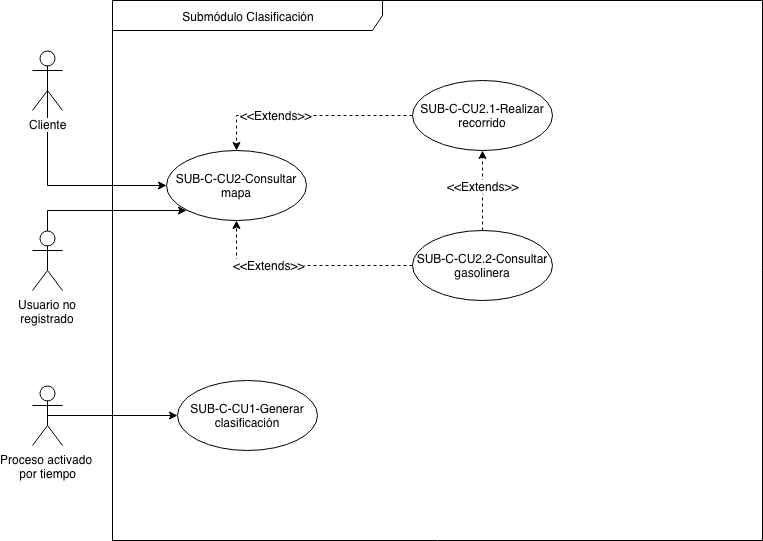
\includegraphics[scale=.6]{Capitulo4/software/submodulos/clasificacion/images/dcu}
	\caption{Diagrama de casos de uso del submódulo Clasificación}
	\label{fig:dcu-clasificacion}
\end{figure}
\newpage
\subsubsection{SUB-C-CU1-Generar clasificación}\label{SUB-C-CU1}
Proceso que se ejecuta cada determinado tiempo para realizar una actualización de la clasificación de las gasolineras.

\begin{longtable}{|J{5cm}|J{10.3cm}|}
	\hline
	\textbf{Nombre del caso de uso} &
		SUB-C-CU1-Generar clasificación \\ \hline
	\textbf{Objetivo} &
		Actualizar la clasificación de gasolineras \\ \hline
	\textbf{Actores} &
		Proceso en el tiempo \\ \hline 
	\textbf{Disparador} & 
		Se cumple el tiempo establecido. \\ \hline 
	\textbf{Entradas} & 
		\begin{itemize}
				\item Listado de gasolineras.
				\item Mediciones.
		\end{itemize}\\ \hline 
	\textbf{Salidas} & 
		\begin{itemize}
			\item Listado de gasolineras actualizado.
		\end{itemize} \\ \hline
	\textbf{Precondiciones} &
		Ninguna.\\ \hline
	\textbf{Postcondiciones} &
		\begin{itemize}
			\item La clasificación actualiza puede ser consultada por los usuarios.
		\end{itemize} \\ \hline
	\textbf{Condiciones de término} & 
		\begin{itemize}
			\item Termina su ejecución el algoritmos clasificatorio.
		\end{itemize} \\ \hline 
	\textbf{Prioridad} & 
		Alta. \\ \hline
	\textbf{Errores} & Ninguno.
		% \begin{itemize}
		% 	\item \label{SUB-M-CU1:Error1} Error 1: .
		% \end{itemize} 
		\\ \hline
	\textbf{Reglas de negocio} & 
		\begin{itemize}
			\item \ref{RN7}.
			\item \ref{RN8}.
		\end{itemize}
		 \\ \hline
	% \caption{}
	%\label{desc:SUB-M-CU1}
\end{longtable}

\paragraph{Trayectoria principal}
	\begin{enumerate}
		\item {[Sistema]} Verifica que se haya cumplido el tiempo especifico para que se actualice la clasificación de gasolineras con base en lo establecido en la regla de negocio \ref{RN7}.
		\item {[Sistema]} Obtiene el listado de gasolineras registradas.
		\item {[Sistema]} Obtiene las mediciones registradas para cada una de las gasolineras obtenidas.
		\item {[Sistema]} Ejecuta el algoritmos de clasificación especificado en la regla de negocio \ref{RN8}.
		\item {[Sistema]} Persiste la clasificación calculada.
	\end{enumerate}
	Fin del caso de uso.

% \paragraph{Trayectoria alternativa A} \label{SUB-M-CU1.1:TA}
% 	El actor no se encuentra usando la aplicación móvil.
% 	\begin{enumerate}[label=A\arabic*.]
% 		\item {[Sistema]} Muestra una notificación al actor como la que se observa en la pantalla \hyperref[fig:sub-m-iu1.1.a]{SUB-M-IU1.1-Confirmar medición (a)}.
% 		\item {[Actor]} Presiona la notificación.
% 		\item {[Sistema]} Continúa en el paso \ref{SUB-M-CU1.1:Pantalla} de la Trayectoria Principal.
% 	\end{enumerate}
% 	Fin de la trayectoria alternativa.

% \paragraph{Puntos de extensión} \label{SUB-M-CU1.1:P}
% \begin{enumerate}[label=PE\arabic*.]
% 	\item Caso de uso \hyperref[SUB-M-CU1.1.3]{SUB-M-CU1.1.3-Obtener insignia} en el paso \ref{SUB-M-CU1.1:Boton} de la Trayectoria principal.
% 	\item Caso de uso \hyperref[SUB-M-CU1.1.4]{SUB-M-CU1.1.4-Asignar insignia a gasolinera} en el paso \ref{SUB-M-CU1.1:Boton} de la Trayectoria principal.
% 	\item Caso de uso \hyperref[SUB-M-CU1.1.5]{SUB-M-CU1.1.5-Especificar bomba} en el paso \ref{SUB-M-CU1.1:Boton} de la Trayectoria principal.
% \end{enumerate}

\subsubsection{SUB-C-CU2-Consultar mapa}\label{SUB-C-CU2}
Cuando el actor abre la aplicación móvil, se le muestra en un mapa su ubicación, junto con la ubicación de gasolineras que tenga cercanas. De estás gasolineras se muestra su dirección y su clasificación.

\begin{longtable}{|J{5cm}|J{10.3cm}|}
	\hline
	\textbf{Nombre del caso de uso} &
		SUB-C-CU2-Consultar mapa \\ \hline
	\textbf{Objetivo} &
		Mostrar al actor las gasolineras cercanas a él, además de la clasificación de las mismas. \\ \hline
	\textbf{Actores} &
		\begin{itemize}
			\item Cliente.
			\item Usuario no registrado.
		\end{itemize}
		 \\ \hline 
	\textbf{Disparador} & 
		El actor ingresa a la aplicación móvil. \\ \hline
	\textbf{Entradas} & 
		\begin{itemize}
				\item Ubicación del actor.
		\end{itemize}\\ \hline 
	\textbf{Salidas} & 
		\begin{itemize}
			\item Mapa que muestra las gasolineras cercanas a él, al igual que la clasificación y dirección de las mismas.
		\end{itemize} \\ \hline
	\textbf{Precondiciones} &
		Ninguna.\\ \hline
	\textbf{Postcondiciones} &
		\begin{itemize}
			\item El actor puede seleccionar una gasolinera de las que le aparecen en el mapa.
		\end{itemize} \\ \hline
	\textbf{Condiciones de término} & 
		\begin{itemize}
			\item Se muestra el mapa con la clasificación de gasolinera al actor.
		\end{itemize} \\ \hline 
	\textbf{Prioridad} & 
		Alta. \\ \hline
	\textbf{Errores} & Ninguno.
		% \begin{itemize}
		% 	\item \label{SUB-M-CU1:Error1} Error 1: .
		% \end{itemize} 
		\\ \hline
	\textbf{Reglas de negocio} & \ref{RN9}.
		% \begin{itemize}
		% 	\item \ref{RN1}.
		% \end{itemize}
		 \\ \hline
	% \caption{}
	%\label{desc:SUB-M-CU1}
\end{longtable}

\paragraph{Trayectoria principal}
	\begin{enumerate}
		\item {[Actor]} Abre la aplicación móvil.
		\item {[Sistema]} Obtiene la ubicación del usuario.
		\item {[Sistema]} Obtiene las gasolineras que se encuentran en un radio establecido por la regla de negocio \ref{RN9}.
		\item {[Sistema]} De las gasolineras cercanas al actor, obtiene la clasificación y dirección de las mismas.
		\item {[Sistema]} Consulta el api de Google Maps y marca las gasolineras.
		\item \label{SUB-C-CU2:Pantalla} {[Sistema]} Muestra la información obtenida en la pantalla \hyperref[fig:sub-c-iu2]{SUB-C-IU2-Consultar mapa}.
	\end{enumerate}
	Fin del caso de uso.

\paragraph{Puntos de extensión} \label{SUB-C-CU2:PE}
\begin{enumerate}[label=PE\arabic*.]
	\item Caso de uso \hyperref[SUB-C-CU2.1]{SUB-C-CU2.1-Realizar recorrido} en el paso \ref{SUB-C-CU2:Pantalla} de la Trayectoria principal.
	\item Caso de uso \hyperref[SUB-C-CU2.2]{SUB-C-CU2.2-Consultar gasolinera} en el paso \ref{SUB-C-CU2:Pantalla} de la Trayectoria principal.
\end{enumerate}

\subsubsection{SUB-C-CU2.1-Realizar recorrido}\label{SUB-C-CU2.1}
El actor puede seleccionar una gasolinera, y el sistema le mostrará una ruta que pueda seguir para llegar hasta ella.

\begin{longtable}{|J{5cm}|J{10.3cm}|}
	\hline
	\textbf{Nombre del caso de uso} &
		SUB-C-CU2.1-Realizar recorrido \\ \hline
	\textbf{Objetivo} &
		Guiar al actor hasta una gasolinera que el haya seleccionado \\ \hline
	\textbf{Actores} &
		\begin{itemize}
			\item Cliente.
			\item Usuario no registrado.
		\end{itemize}
		 \\ \hline 
	\textbf{Disparador} & 
		El actor presiona el icono \textit{¿Cómo llegar?}. \\ \hline 
	\textbf{Entradas} & 
		\begin{itemize}
				\item Gasolinera seleccionada.
		\end{itemize}\\ \hline 
	\textbf{Salidas} & 
		\begin{itemize}
			\item Ruta.
		\end{itemize} \\ \hline
	\textbf{Precondiciones} &
		Deben existir gasolineras en el sistema.\\ \hline
	\textbf{Postcondiciones} & Ninguna.
		% \begin{itemize}
		% 	\item Nin
		% \end{itemize} 
		\\ \hline
	\textbf{Condiciones de término} & 
		\begin{itemize}
			\item Se le muestra al actor la ruta trazada en el mapa.
		\end{itemize} \\ \hline 
	\textbf{Prioridad} & 
		Media. \\ \hline
	\textbf{Errores} & Ninguno.
		% \begin{itemize}
		% 	\item \label{SUB-M-CU1:Error1} Error 1: .
		% \end{itemize} 
		\\ \hline
	\textbf{Reglas de negocio} & Ninguna.
		% \begin{itemize}
		% 	\item \ref{RN1}.
		% \end{itemize}
		 \\ \hline
	% \caption{}
	%\label{desc:SUB-M-CU1}
\end{longtable}

\paragraph{Trayectoria principal}
	\begin{enumerate}
		\item {[Actor]} Presiona el icono \textit{Realizar recorrido} en la pantalla \hyperref[fig:sub-c-iu2]{SUB-C-IU2-Consultar mapa}.
		\item {[Actor]} Selecciona una gasolinera.
		\item {[Sistema]} Obtiene del api de Google Maps la ruta para llegar a la gasolinera seleccionada.
		\item {[Sistema]} Muestra la ruta en la pantalla \hyperref[fig:sub-c-iu2.1]{SUB-C-IU2.1-Realizar recorrido}.
	\end{enumerate}
	Fin del caso de uso.

% \paragraph{Trayectoria alternativa A} \label{SUB-M-CU1.1:TA}
% 	El actor no se encuentra usando la aplicación móvil.
% 	\begin{enumerate}[label=A\arabic*.]
% 		\item {[Sistema]} Muestra una notificación al actor como la que se observa en la pantalla \hyperref[fig:sub-m-iu1.1.a]{SUB-M-IU1.1-Confirmar medición (a)}.
% 		\item {[Actor]} Presiona la notificación.
% 		\item {[Sistema]} Continúa en el paso \ref{SUB-M-CU1.1:Pantalla} de la Trayectoria Principal.
% 	\end{enumerate}
% 	Fin de la trayectoria alternativa.

\subsubsection{SUB-C-CU2.2-Consultar gasolinera}\label{SUB-C-CU2.2}
El actor puede consultar información especifica de cada gasolinera al presionar sobre alguna de ellas.

\begin{longtable}{|J{5cm}|J{10.3cm}|}
	\hline
	\textbf{Nombre del caso de uso} &
		SUB-M-CU2.2-Consultar gasolinera \\ \hline
	\textbf{Objetivo} &
		Permitir al actor, obtener información especifica sobre alguna de las gasolineras. \\ \hline
	\textbf{Actores} &
		\begin{itemize}
			\item Cliente.
			\item Usuario no registrado.
		\end{itemize}
		 \\ \hline 
	\textbf{Disparador} & 
		El actor presiona sobre el icono de una gasolinera. \\ \hline 
	\textbf{Entradas} & 
		\begin{itemize}
				\item Gasolinera seleccionada.
		\end{itemize}\\ \hline 
	\textbf{Salidas} & 
		\begin{itemize}
			\item Información de la gasolinera.
			\item Insignias asociadas a la gasolinera.
		\end{itemize} \\ \hline
	\textbf{Precondiciones} &
		Deben existir gasolineras en el sistema.\\ \hline
	\textbf{Postcondiciones} & Ninguna.
		% \begin{itemize}
		% 	\item La medición calculada puede ser consultada por el Cliente.
		% 	\item La medición se usa en el algoritmo de clasificación.
		% \end{itemize} 
		\\ \hline
	\textbf{Condiciones de término} & 
		\begin{itemize}
			\item Se le muestra al actor la información de la gasolinera seleccionada.
		\end{itemize} \\ \hline 
	\textbf{Prioridad} & 
		Alta. \\ \hline
	\textbf{Errores} & Ninguno.
		% \begin{itemize}
		% 	\item \label{SUB-M-CU1:Error1} Error 1: .
		% \end{itemize} 
		\\ \hline
	\textbf{Reglas de negocio} & Ninguna.
		% \begin{itemize}
		% 	\item \ref{RN1}.
		% \end{itemize}
		 \\ \hline
	% \caption{}
	%\label{desc:SUB-M-CU1}
\end{longtable}

\paragraph{Trayectoria principal}
	\begin{enumerate}
		\item {[Actor]} Presiona sobre el icono de una gasolinera.
		\item {[Sistema]} Obtiene la gasolinera seleccionada.
		\item {[Sistema]} Obtiene la información de la gasolinera seleccionada.
		\item {[Sistema]} Obtiene la insignias asociadas a la gasolinera.
		\item {[Sistema]} Muestra la información obtenida, en la pantalla \hyperref[fig:sub-c-iu2.2]{SUB-C-IU2.2-Consultar gasolinera}.
	\end{enumerate}
	Fin del caso de uso.

% \paragraph{Trayectoria alternativa A} \label{SUB-M-CU1.1:TA}
% 	El actor no se encuentra usando la aplicación móvil.
% 	\begin{enumerate}[label=A\arabic*.]
% 		\item {[Sistema]} Muestra una notificación al actor como la que se observa en la pantalla \hyperref[fig:sub-m-iu1.1.a]{SUB-M-IU1.1-Confirmar medición (a)}.
% 		\item {[Actor]} Presiona la notificación.
% 		\item {[Sistema]} Continúa en el paso \ref{SUB-M-CU1.1:Pantalla} de la Trayectoria Principal.
% 	\end{enumerate}
% 	Fin de la trayectoria alternativa.



\subsection{Menús de usuario}
\subsubsection{Interfaces de Usuario}\label{Interfaces de Usuario}

\begin{enumerate}[label=IU\arabic*.]
    \item  
    \begin{figure}[H]
	\centering
	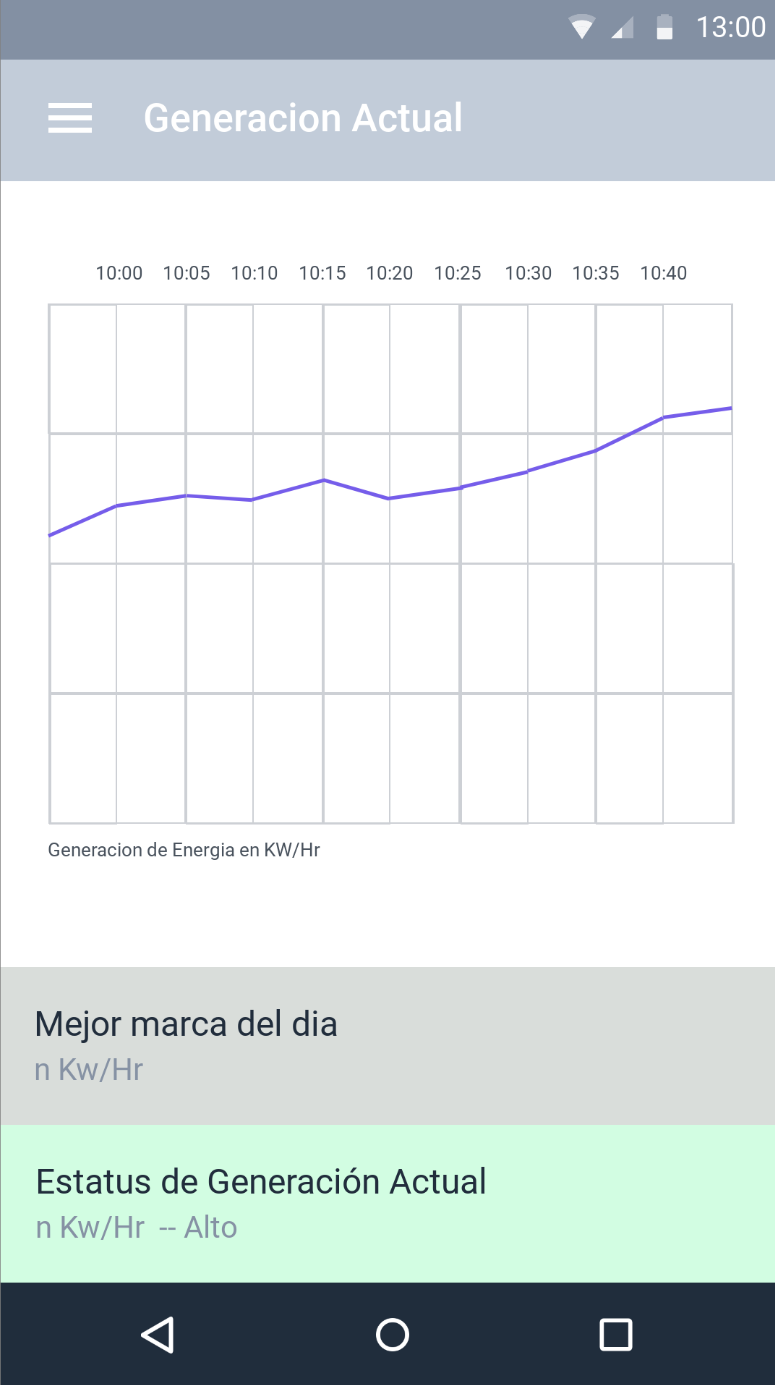
\includegraphics[scale=0.70]{Capitulo4/software/submodulos/images/monitoreo.png}
	\caption{Interfaz de usuario IU1-Monitoreo En Tiempo real}
	\label{fig:monitoreo}
    \end{figure}
		
\end{enumerate}

\begin{figure}[H]
	\centering
	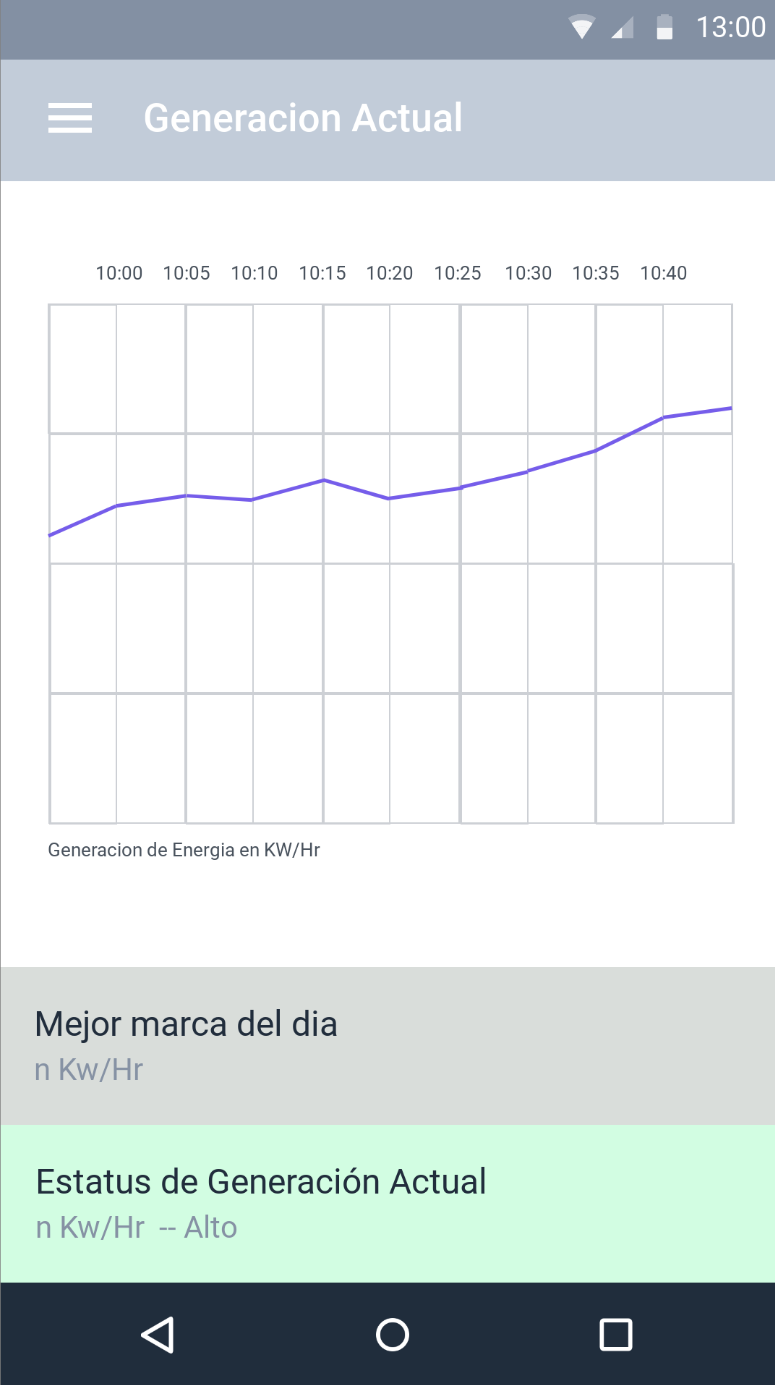
\includegraphics[scale=0.70]{Capitulo4/software/submodulos/images/monitoreo.png}
	\caption{Interfaz de usuario IU1-Monitoreo En Tiempo real}
	\label{fig:monitoreo}
\end{figure}

\begin{figure}[H]
	\centering
	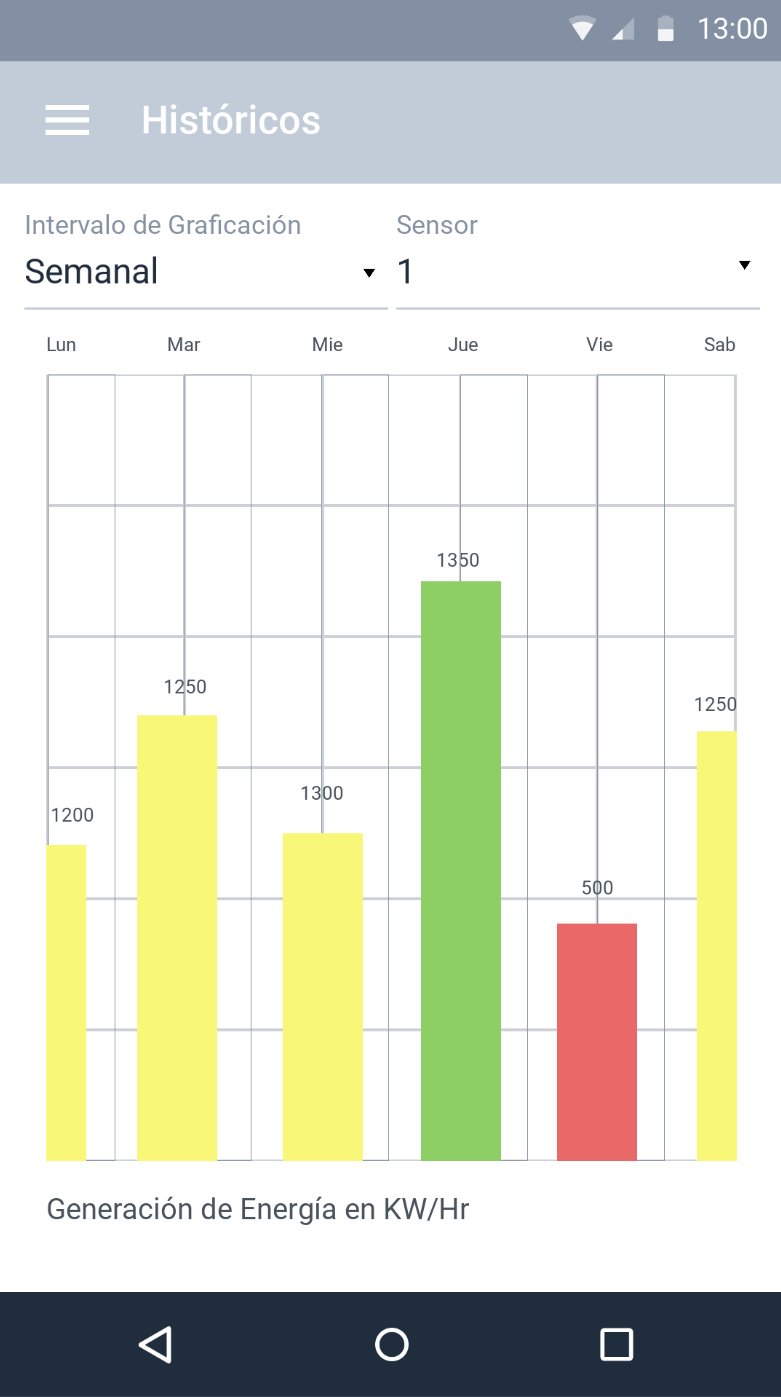
\includegraphics[scale=0.70]{Capitulo4/software/submodulos/images/semanal.png}
	\caption{Interfaz de usuario IU2.1-Historial Semanal}
	\label{fig:Historial Semanal}
\end{figure}

\begin{figure}[H]
	\centering
	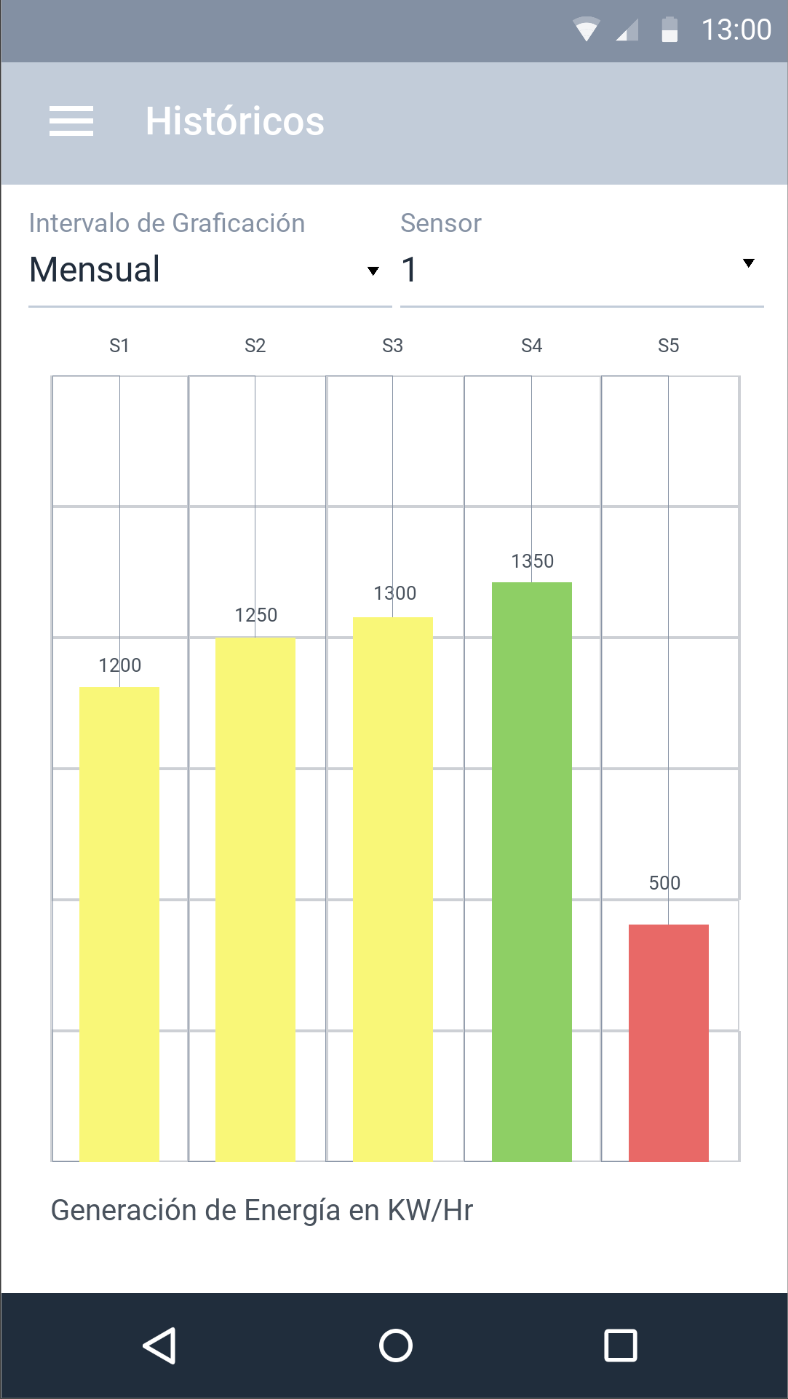
\includegraphics[scale=0.70]{Capitulo4/software/submodulos/images/mensual.png}
	\caption{Interfaz de usuario IU2.2-Historial Mensual}
	\label{fig:Historial Mensual}
\end{figure}

\begin{figure}[H]
	\centering
	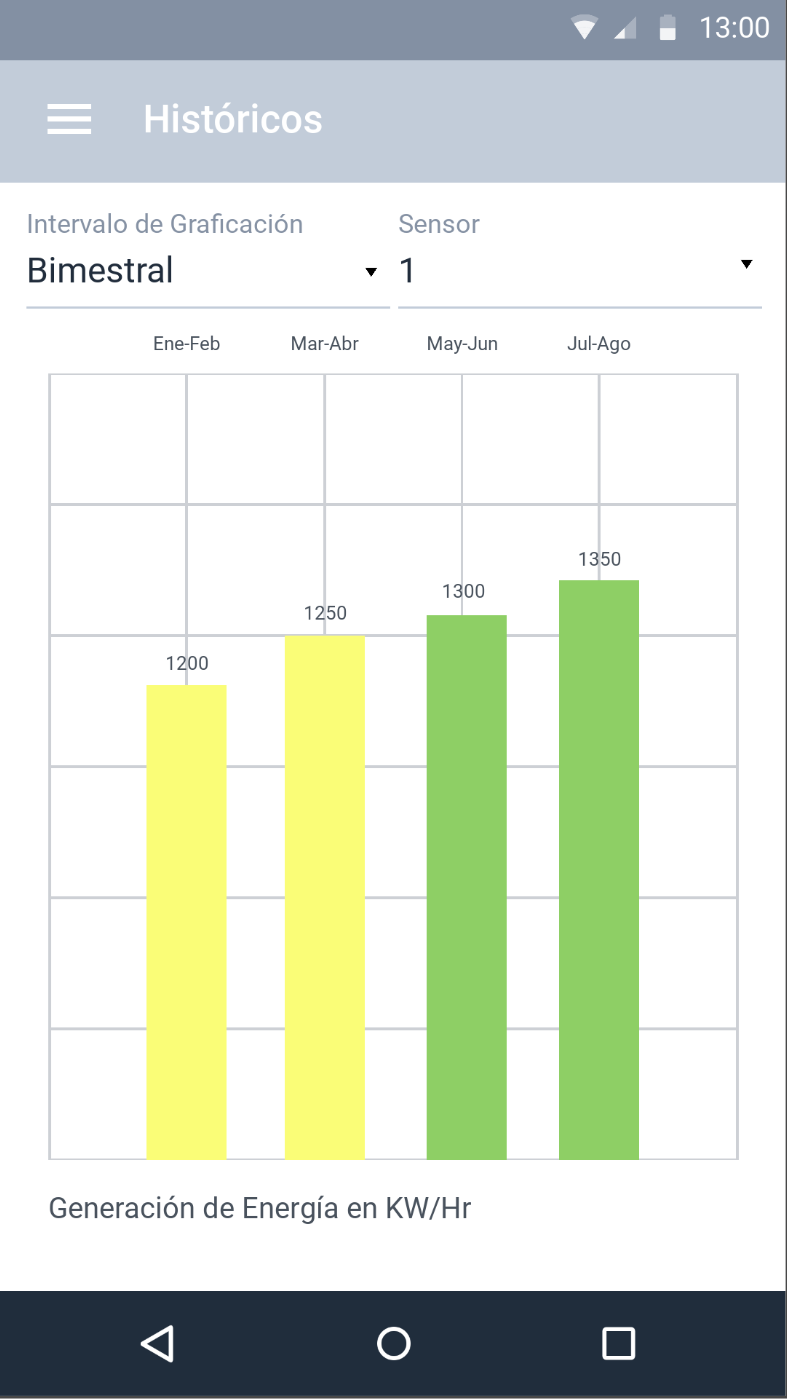
\includegraphics[scale=0.70]{Capitulo4/software/submodulos/images/bimestral.png}
	\caption{Interfaz de usuario IU2.3-Historial Bimestral}
	\label{fig:Historial Bimestral}
\end{figure}

\begin{figure}[H]
	\centering
	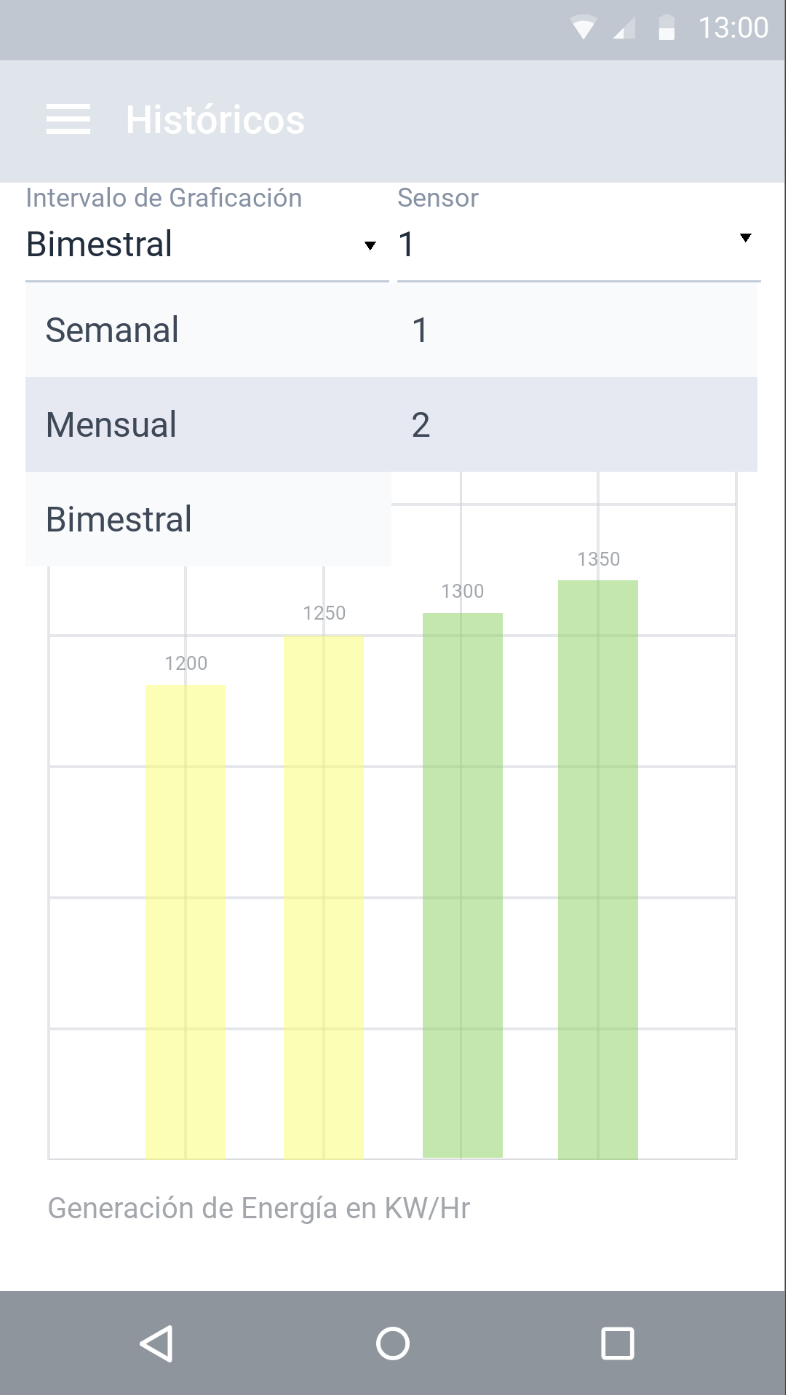
\includegraphics[scale=0.70]{Capitulo4/software/submodulos/images/opciones_hist.png}
	\caption{Interfaz de usuario IU2.4-Opciones de Intervalo}
	\label{fig:Opciones de Intervalo}
\end{figure}

\begin{figure}[H]
	\centering
	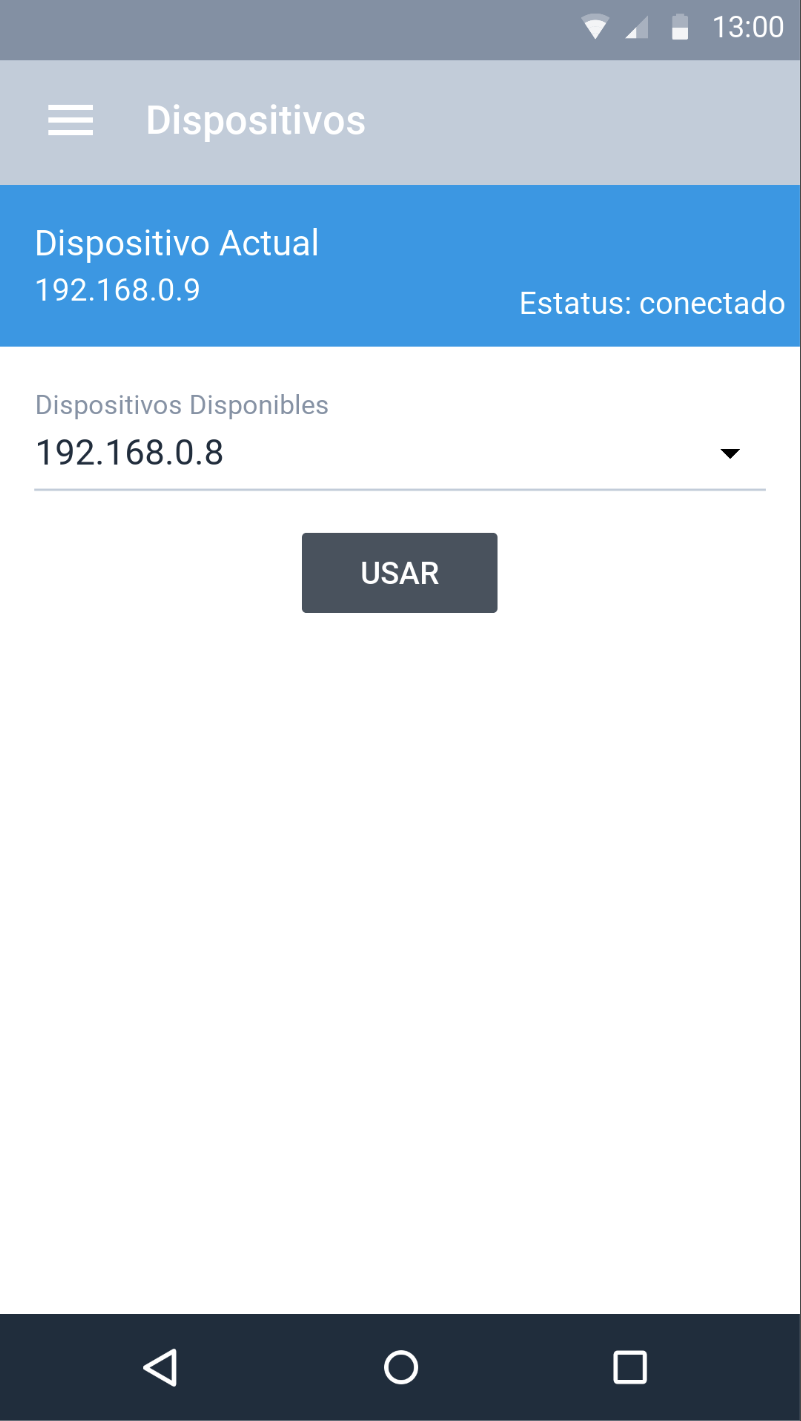
\includegraphics[scale=0.70]{Capitulo4/software/submodulos/images/dispositivos.png}
	\caption{Interfaz de usuario IU3.1-Emparejamiento de Dispositivos}
	\label{fig:Emparejamiento Dispositivos}
\end{figure}

\begin{figure}[H]
	\centering
	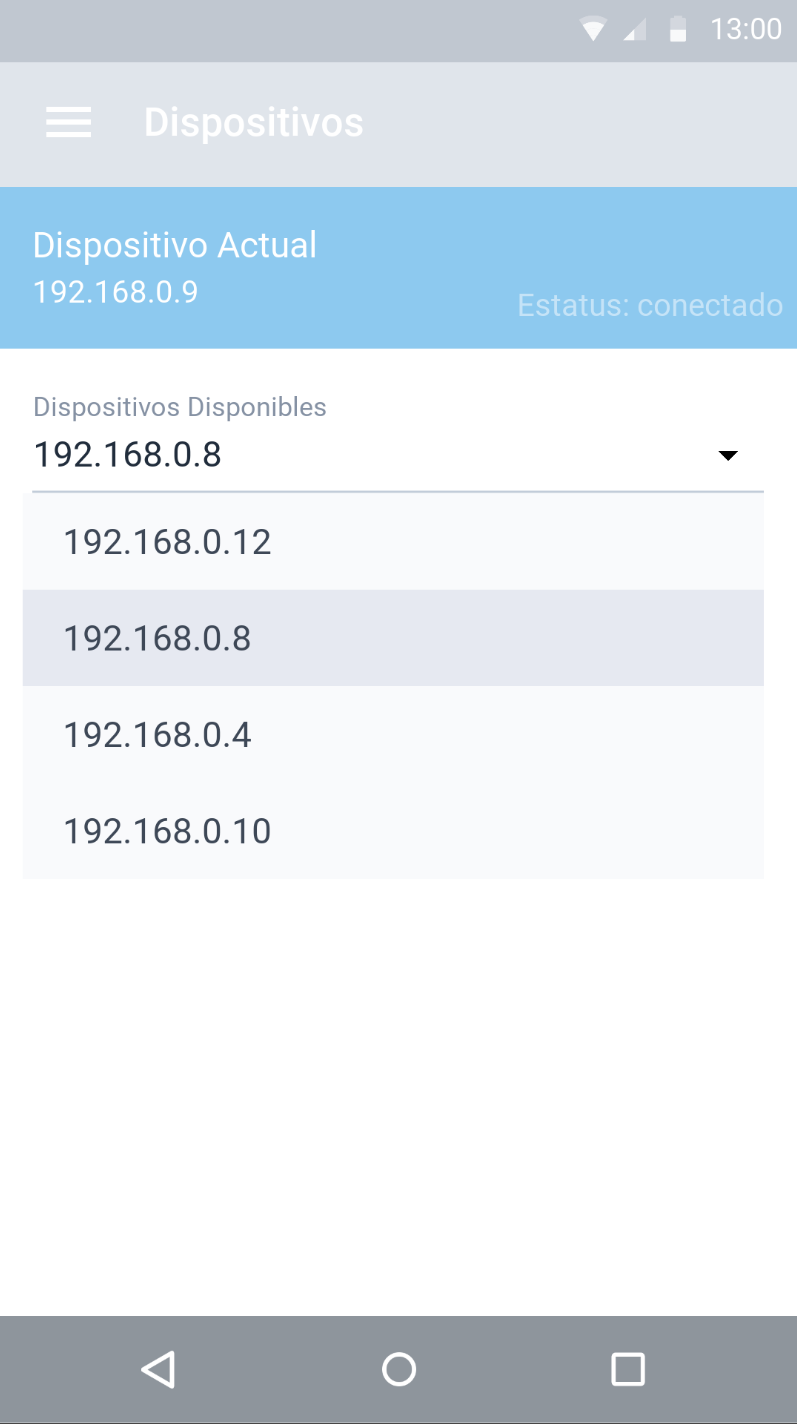
\includegraphics[scale=0.70]{Capitulo4/software/submodulos/images/seleccion_disp.png}
	\caption{Interfaz de usuario IU3.2-Selección de Dispositivo}
	\label{fig:Seleccion de Disposotivo}
\end{figure}

\begin{figure}[H]
	\centering
	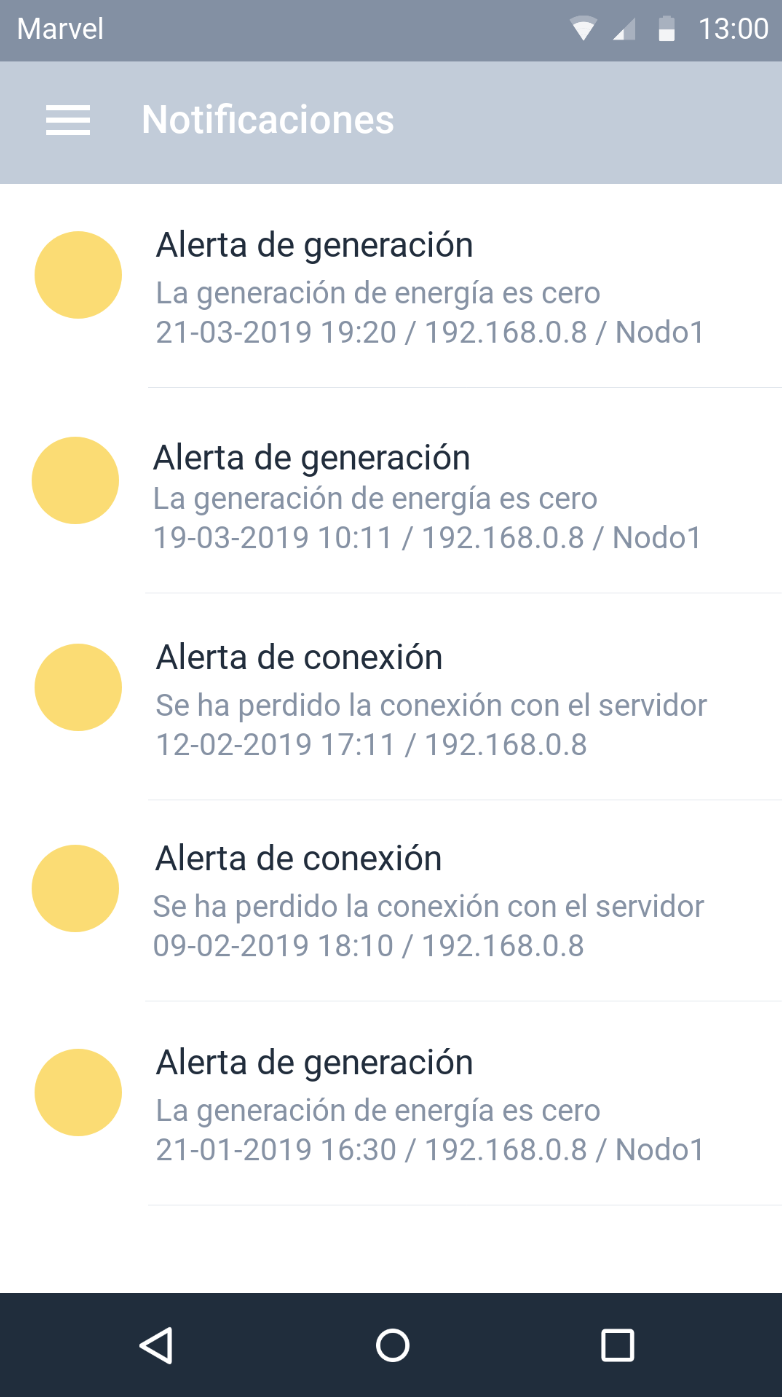
\includegraphics[scale=0.70]{Capitulo4/software/submodulos/images/notificaciones.png}
	\caption{Interfaz de usuario IU4-Lista de Notificaciones}
	\label{fig:Lista de Notificaciones}
\end{figure}

\begin{figure}[H]
	\centering
	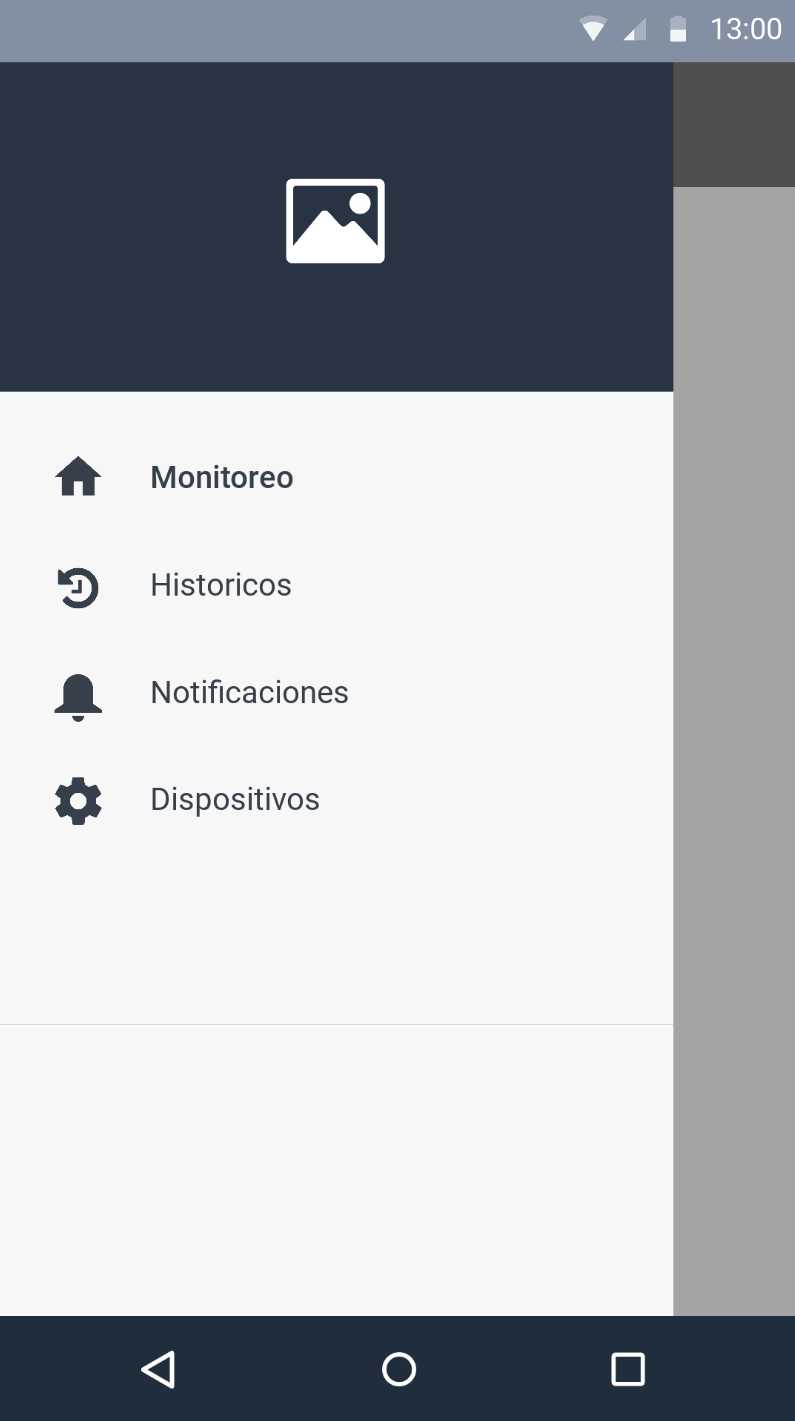
\includegraphics[scale=0.70]{Capitulo4/software/submodulos/images/navegacion.png}
	\caption{Interfaz de usuario IU5-Barra de Navegación}
	\label{fig:Barra de navegacion}
\end{figure}

\subsubsection{Pantallas emergentes}\label{Pantallas Emergentes}

\begin{figure}[H]
	\centering
	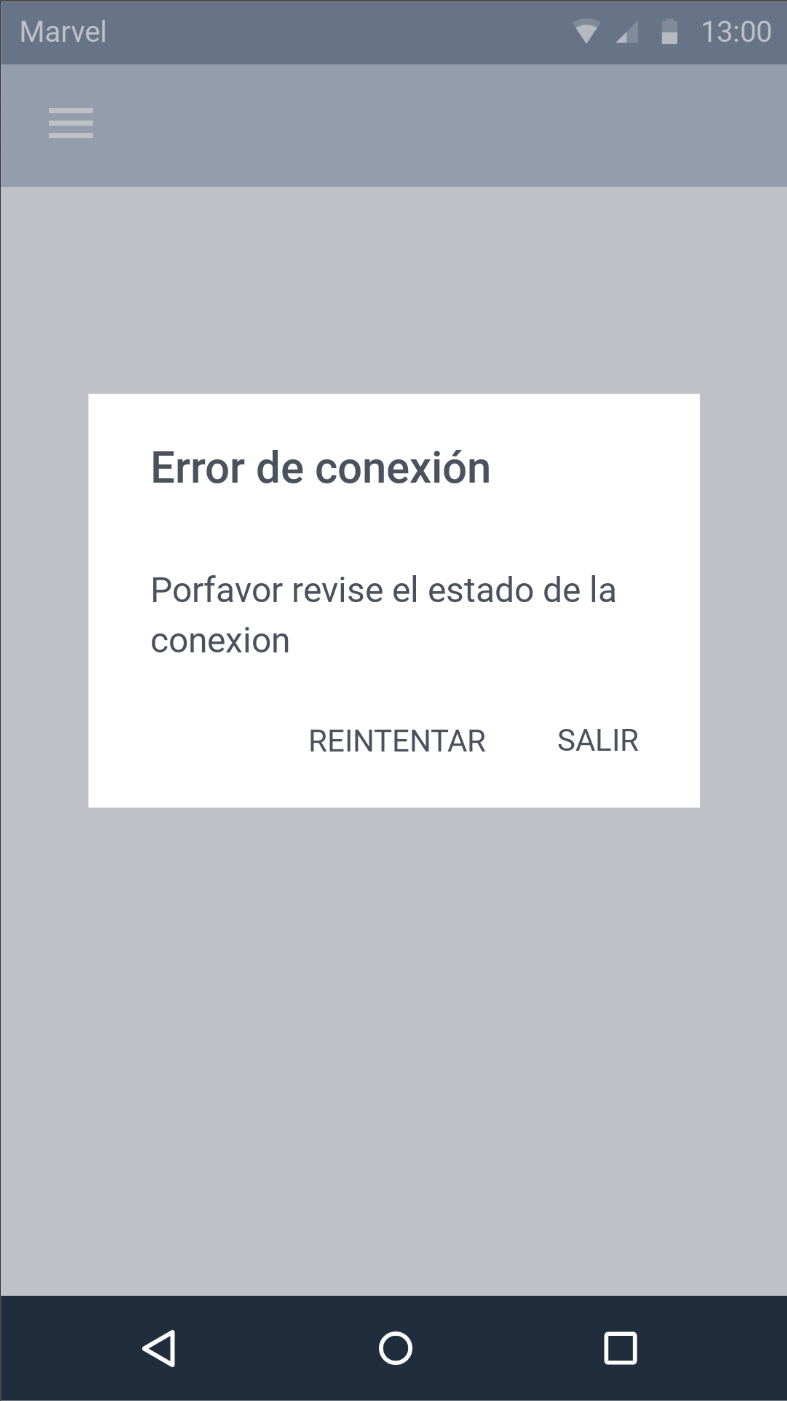
\includegraphics[scale=0.70]{Capitulo4/software/submodulos/images/error_con.png}
	\caption{Pantalla emergente PE1-Error de Conexión}
	\label{fig:Error de Conexion}
\end{figure}

\begin{figure}[H]
	\centering
	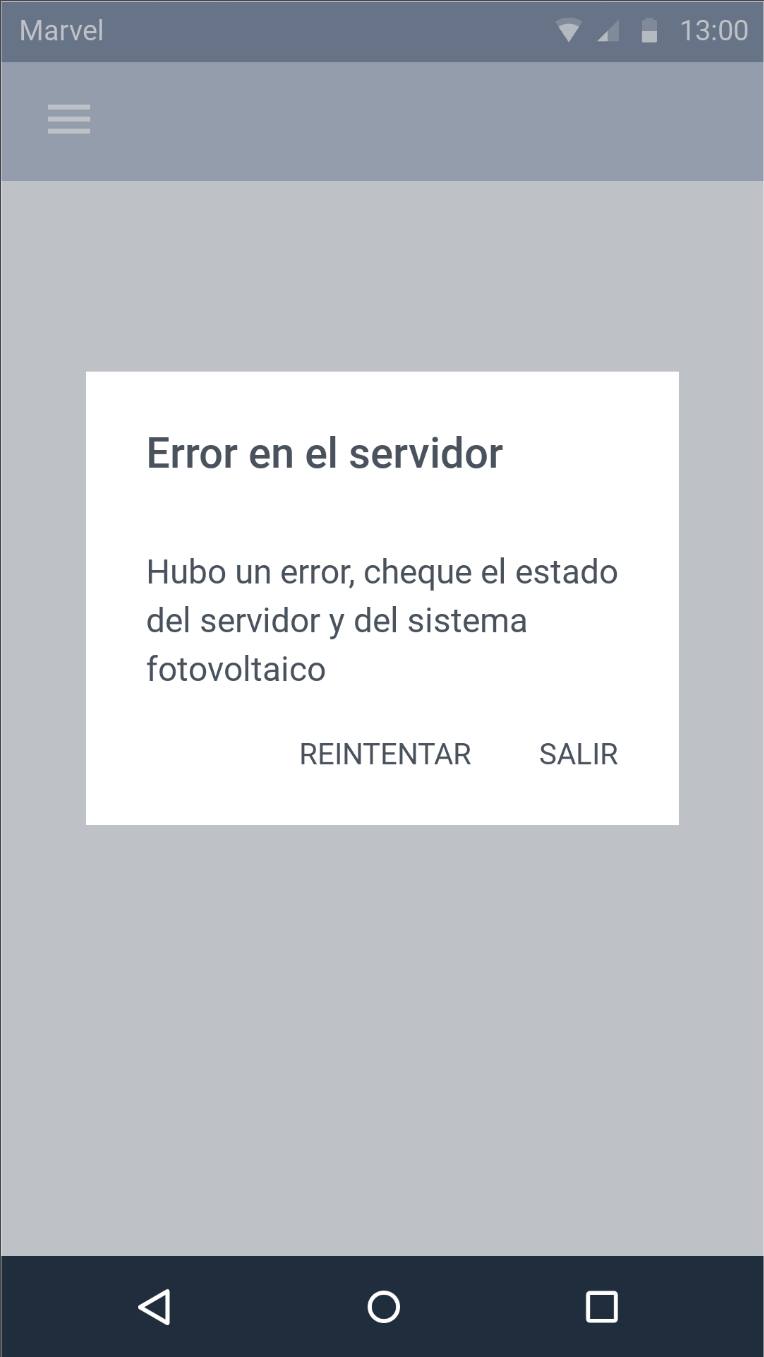
\includegraphics[scale=0.70]{Capitulo4/software/submodulos/images/error_server.png}
	\caption{Pantalla emergente PE2-Error en el Servidor}
	\label{fig:Error en el Servidor}
\end{figure}

\begin{figure}[H]
	\centering
	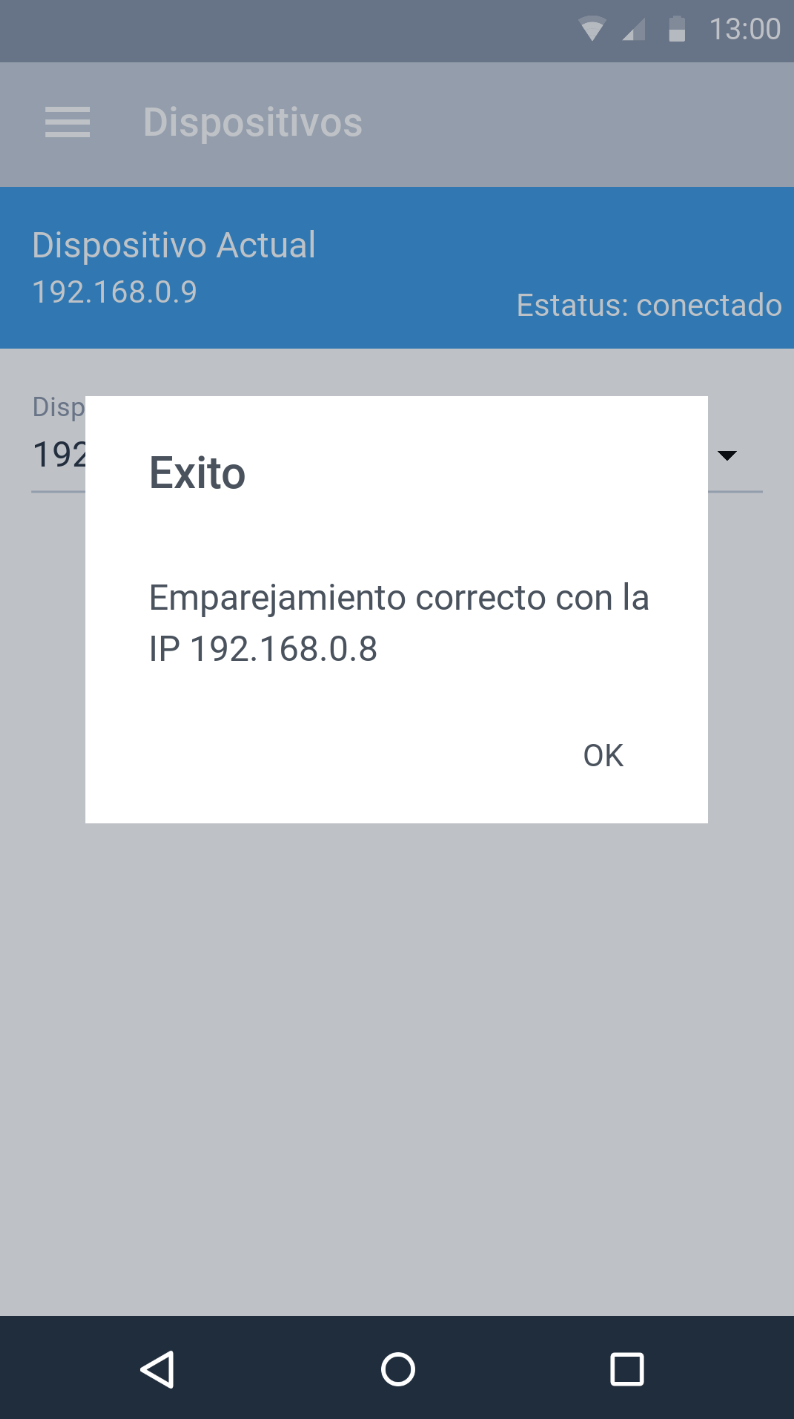
\includegraphics[scale=0.70]{Capitulo4/software/submodulos/images/exito_disp.png}
	\caption{Pantalla emergente PE3-Éxito de Emparejamiento con Dispositivo}
	\label{fig:Exito Emparejamiento}
\end{figure}

\begin{figure}[H]
	\centering
	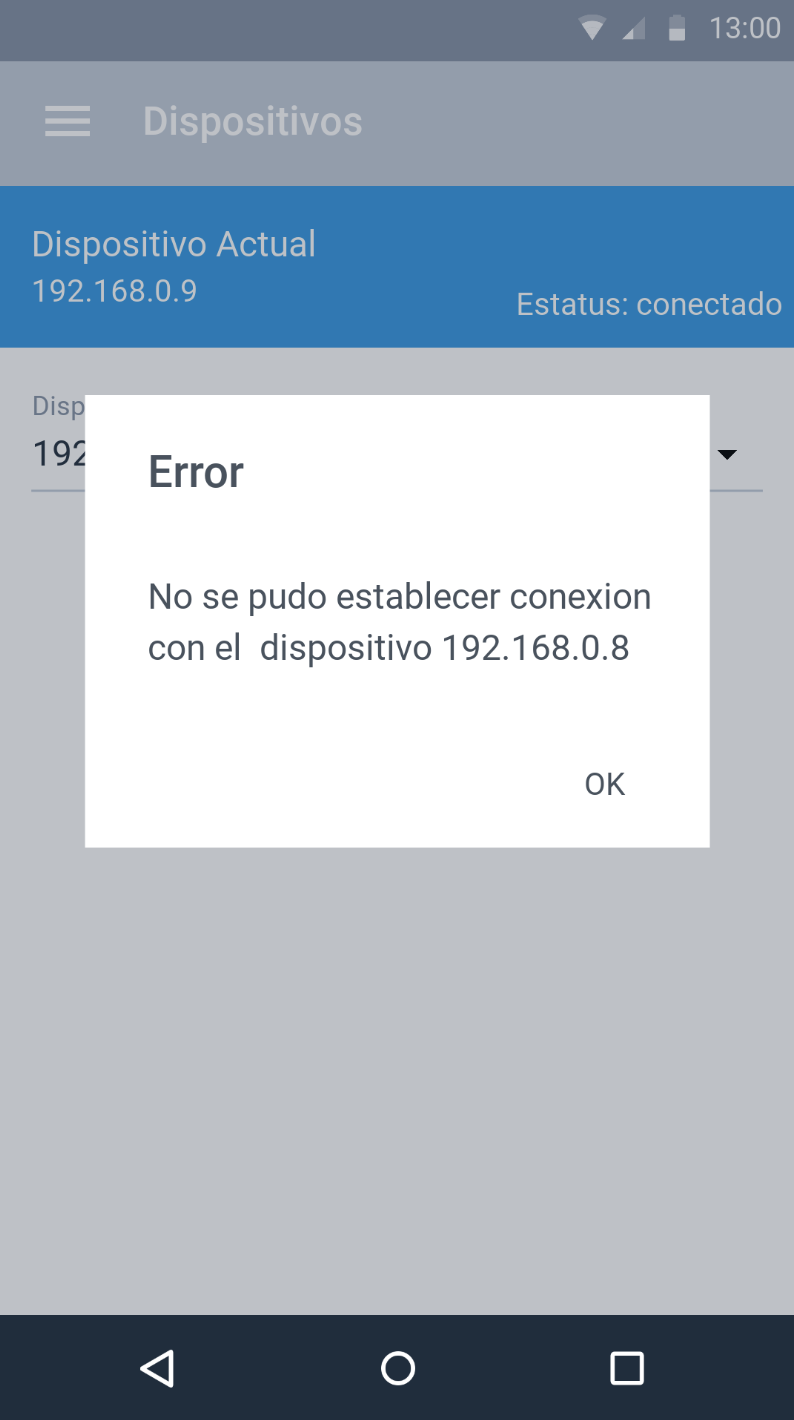
\includegraphics[scale=0.70]{Capitulo4/software/submodulos/images/error_disp.png}
	\caption{Pantalla emergente PE4-Error de Emparejamiento con Dispositivo}
	\label{fig:Error Emparejamiento}
\end{figure}

\subsubsection{Notificaciones}\label{Notificaciones}

\begin{figure}[H]
	\centering
	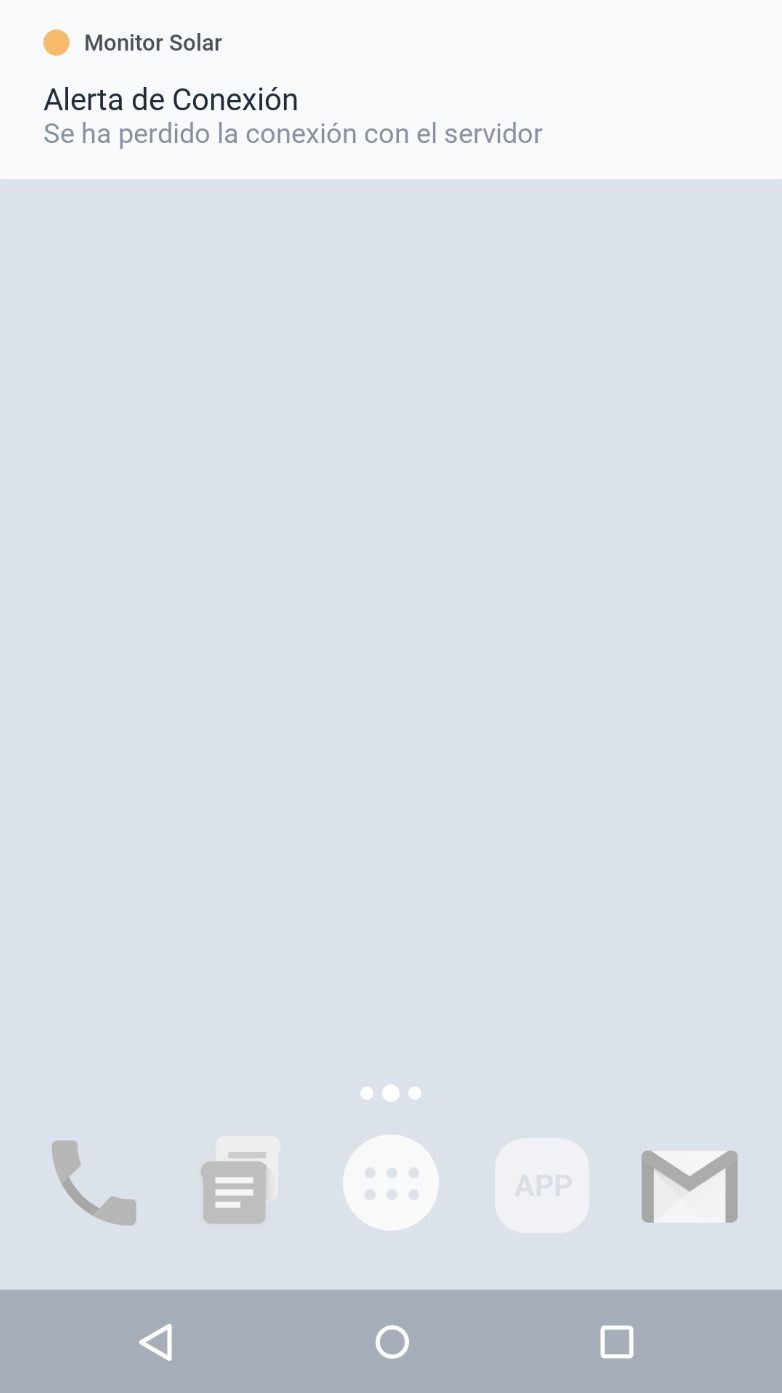
\includegraphics[scale=0.70]{Capitulo4/software/submodulos/images/notif_con.png}
	\caption{Notificación N1-Alerta de Conexión}
	\label{fig:Alerta Conexion}
\end{figure}

\begin{figure}[H]
	\centering
	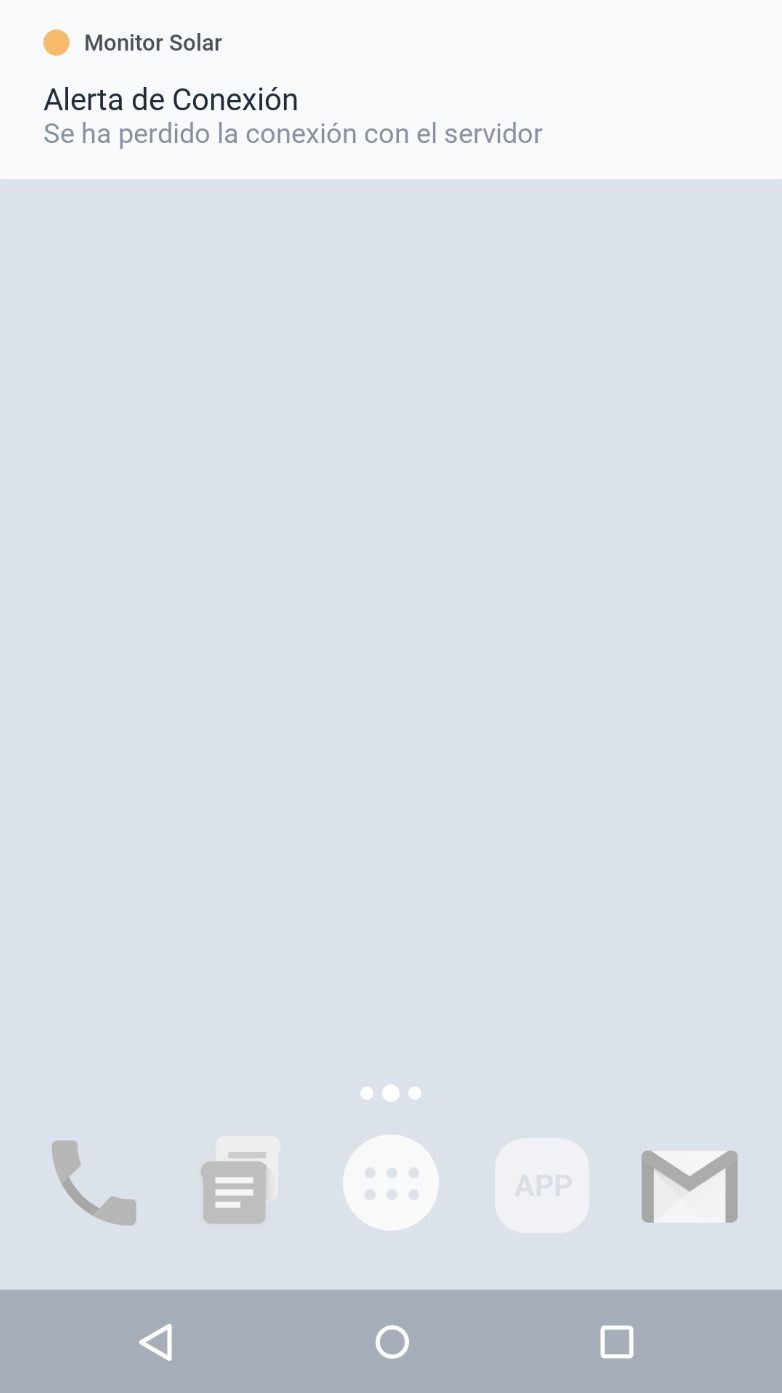
\includegraphics[scale=0.70]{Capitulo4/software/submodulos/images/notif_con.png}
	\caption{Notificación N2-Alerta de Generación}
	\label{fig:Alerta Generacion}
\end{figure}

\begin{figure}[H]
	\centering
	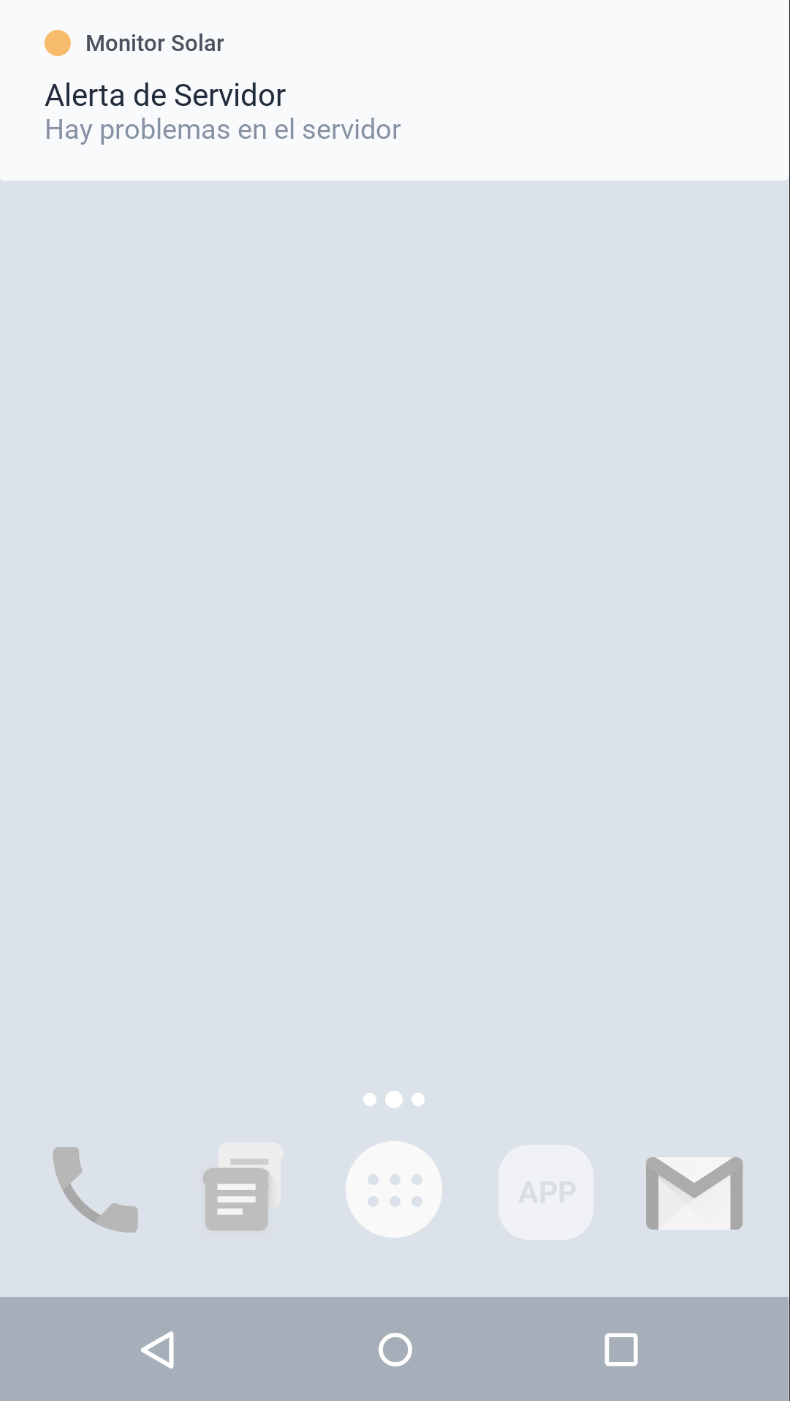
\includegraphics[scale=0.70]{Capitulo4/software/submodulos/images/notif_server.png}
	\caption{Notificación N2-Alerta de Servidor}
	\label{fig:Alerta Servidor}
\end{figure}

\subsection{Interfaces de usuario}
%%%Mediciones
\subsubsection{SUB-M-IU1.1-Confirmar medición}\label{SUB-M-IU1.1}
\begin{figure}[H]
	\centering
	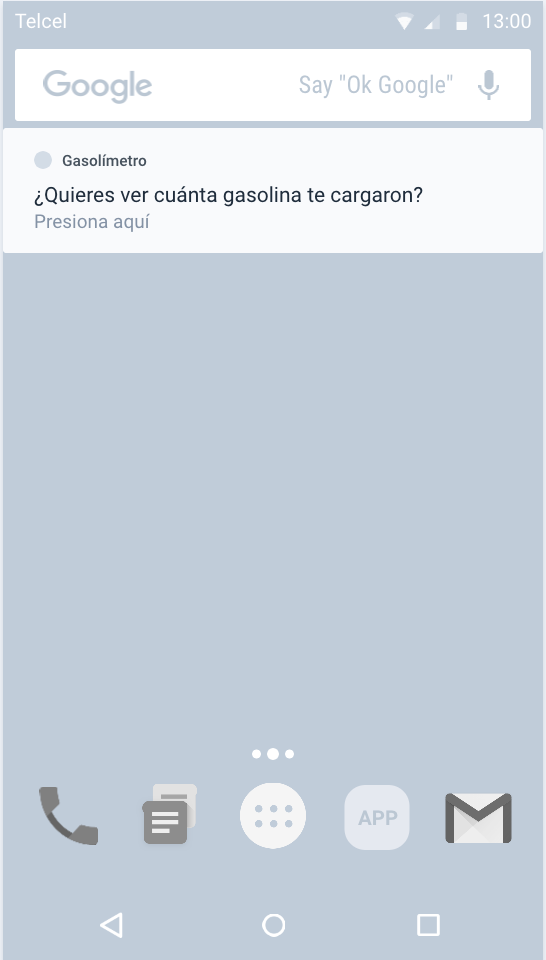
\includegraphics[scale=1]{Capitulo4/software/submodulos/mediciones/images/sub-m-iu1_1_a}
	\caption{Interfaz de usuario SUB-M-IU1.1-Confirmar medición (a)}
	\label{fig:sub-m-iu1.1.a}
\end{figure}

\begin{figure}[H]
	\centering
	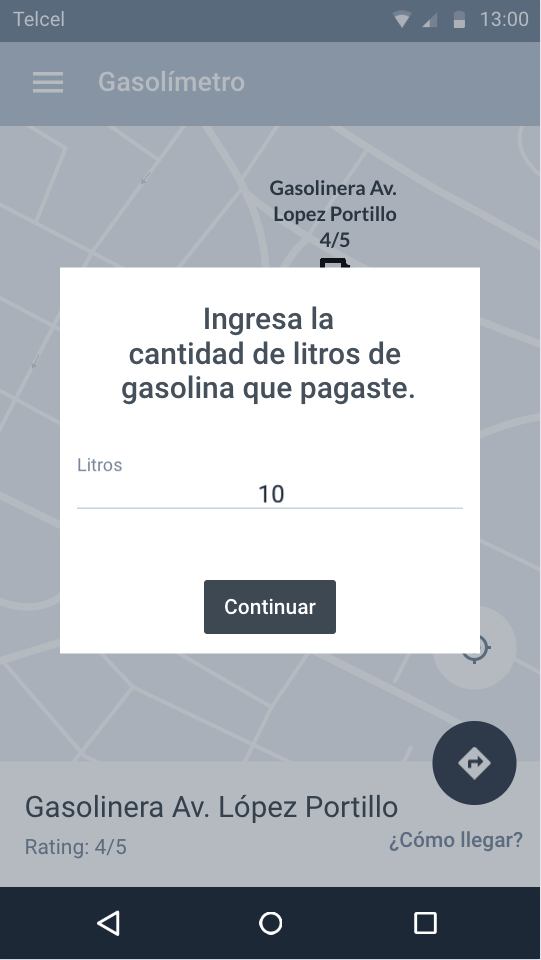
\includegraphics[scale=.55]{Capitulo4/software/submodulos/mediciones/images/sub-m-iu1_1_b}
	\caption{Interfaz de usuario SUB-M-IU1.1-Confirmar medición (b)}
	\label{fig:sub-m-iu1.1.b}
\end{figure}

\begin{figure}[H]
	\centering
	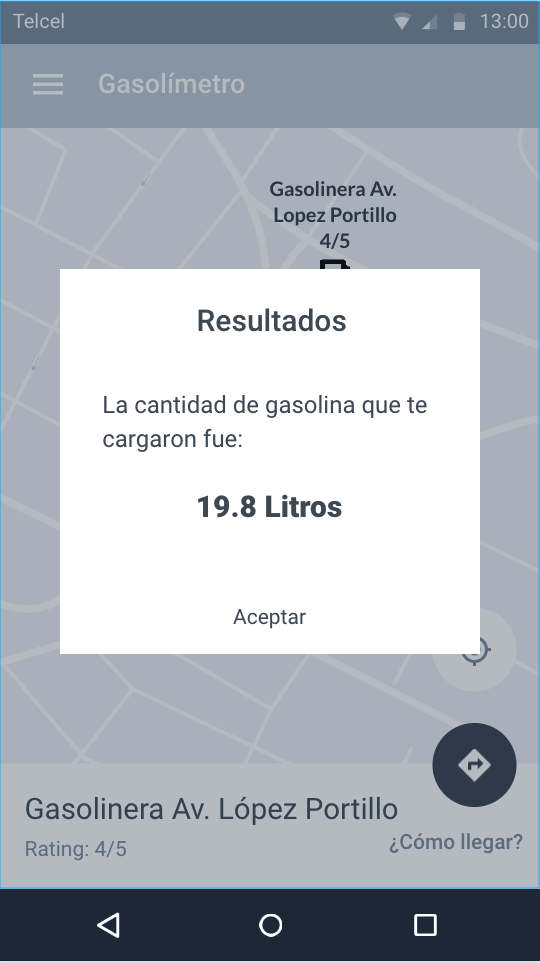
\includegraphics[scale=.55]{Capitulo4/software/submodulos/mediciones/images/sub-m-iu1_1_c}
	\caption{Interfaz de usuario SUB-M-IU1.1-Confirmar medición (c)}
	\label{fig:sub-m-iu1.1.c}
\end{figure}
\subsubsection{SUB-M-IU1.1.2-Registrar precio gasolina}\label{SUB-M-IU1.1.2}
\begin{figure}[H]
	\centering
	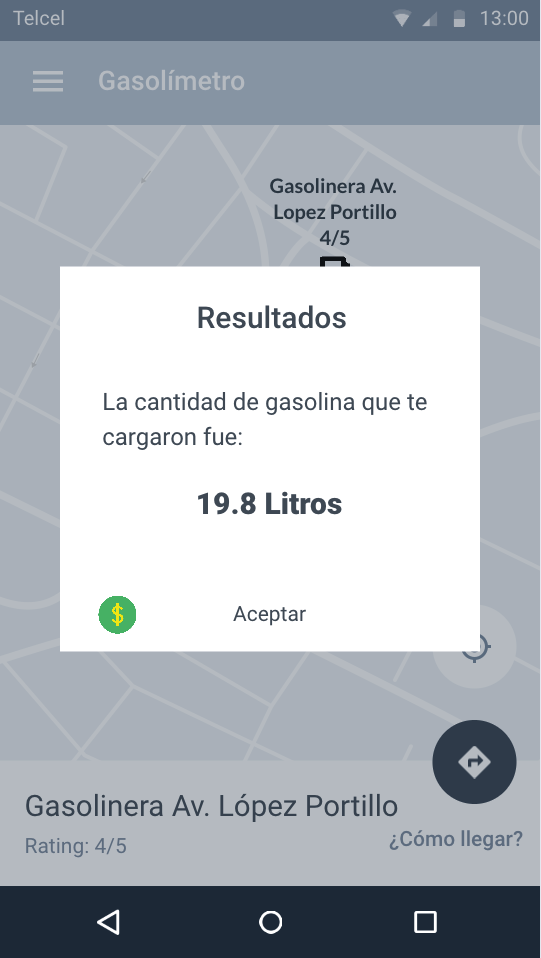
\includegraphics[scale=.55]{Capitulo4/software/submodulos/mediciones/images/sub-m-iu1_1_2_a}
	\caption{Interfaz de usuario SUB-M-IU1.1.2-Registrar precio gasolina (a)}
	\label{fig:sub-m-iu1.1.2.a}
\end{figure}
\begin{figure}[H]
	\centering
	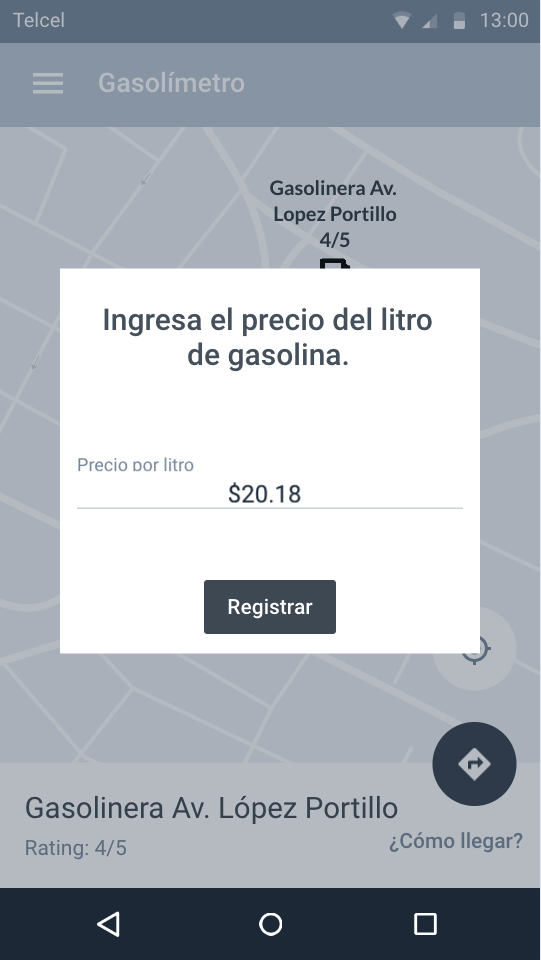
\includegraphics[scale=.55]{Capitulo4/software/submodulos/mediciones/images/sub-m-iu1_1_2_b}
	\caption{Interfaz de usuario SUB-M-IU1.1.2-Registrar precio gasolina (b)}
	\label{fig:sub-m-iu1.1.2.b}
\end{figure}
\subsubsection{SUB-M-IU1.1.3-Obtener insignia}\label{SUB-M-IU1.1.3}
\begin{figure}[H]
	\centering
	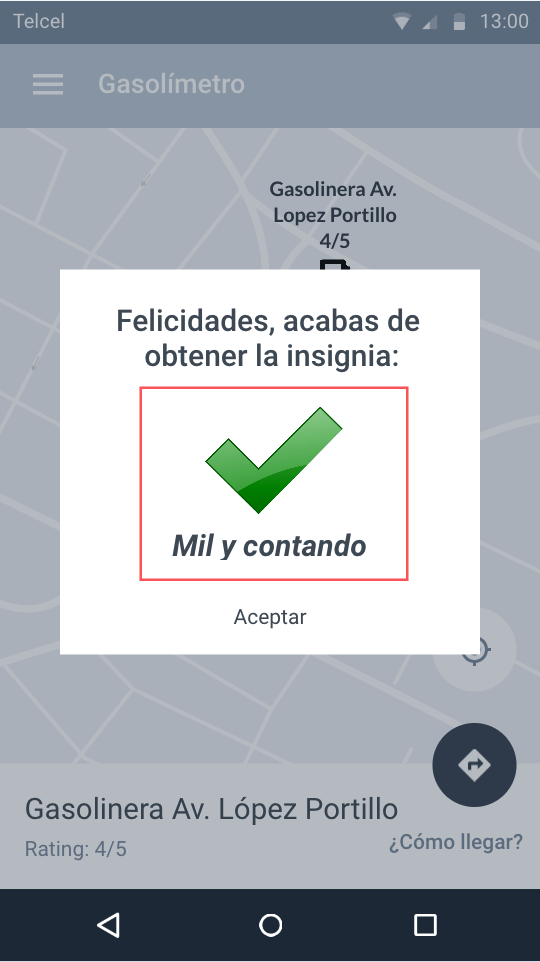
\includegraphics[scale=.55]{Capitulo4/software/submodulos/mediciones/images/sub-m-iu1_1_3}
	\caption{Interfaz de usuario SUB-M-IU1.1.3-Obtener insignia}
	\label{fig:sub-m-iu1.1.3}
\end{figure}
\subsubsection{SUB-M-IU1.1.4-Asignar insignia a gasolinera}\label{SUB-M-IU1.1.4}
\begin{figure}[H]
	\centering
	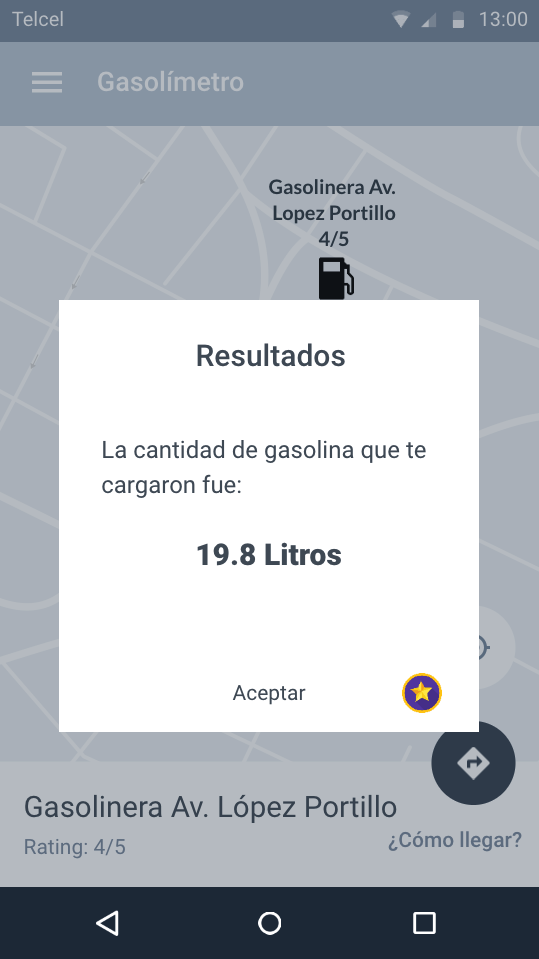
\includegraphics[scale=.55]{Capitulo4/software/submodulos/mediciones/images/sub-m-iu1_1_4_a}
	\caption{Interfaz de usuario SUB-M-IU1.1.4-Asignar insignia a gasolinera (a)}
	\label{fig:sub-m-iu1.1.4.a}
\end{figure}
\begin{figure}[H]
	\centering
	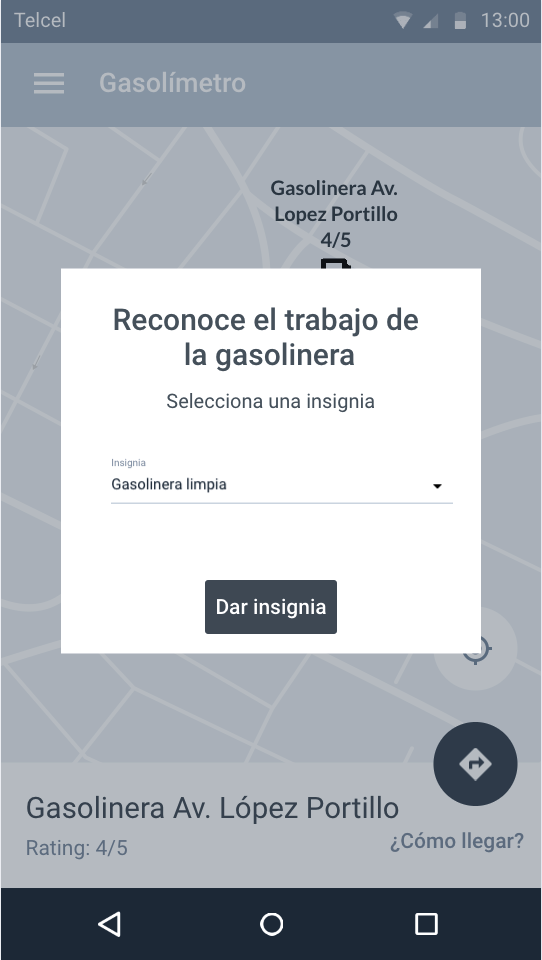
\includegraphics[scale=.55]{Capitulo4/software/submodulos/mediciones/images/sub-m-iu1_1_4_b}
	\caption{Interfaz de usuario SUB-M-IU1.1.4-Asignar insignia a gasolinera (b)}
	\label{fig:sub-m-iu1.1.4.b}
\end{figure}
\subsubsection{SUB-M-IU1.1.5-Especificar bomba}\label{SUB-M-IU1.1.5}
\begin{figure}[H]
	\centering
	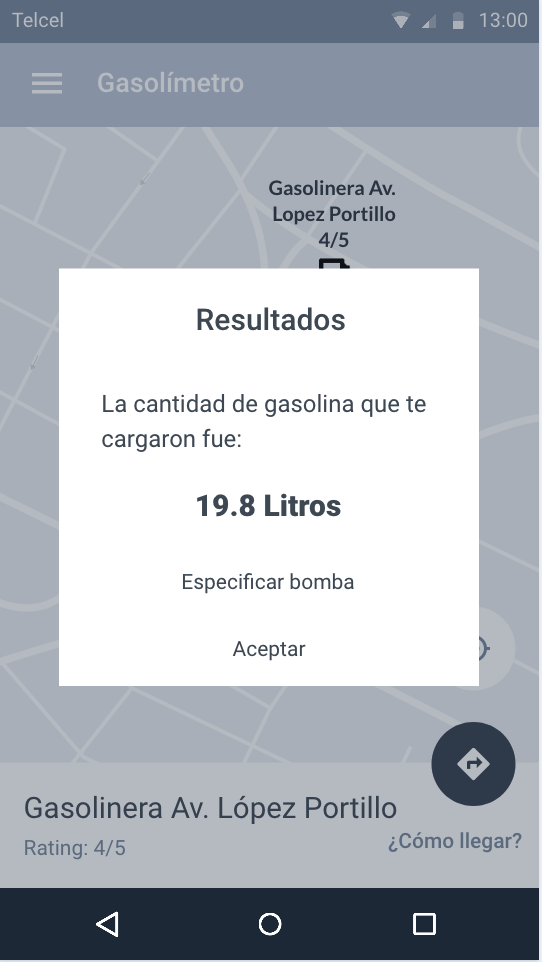
\includegraphics[scale=.55]{Capitulo4/software/submodulos/mediciones/images/sub-m-iu1_1_5_a}
	\caption{Interfaz de usuario SUB-M-IU1.1.5-Especificar bomba (a)}
	\label{fig:sub-m-iu1.1.5.a}
\end{figure}
\begin{figure}[H]
	\centering
	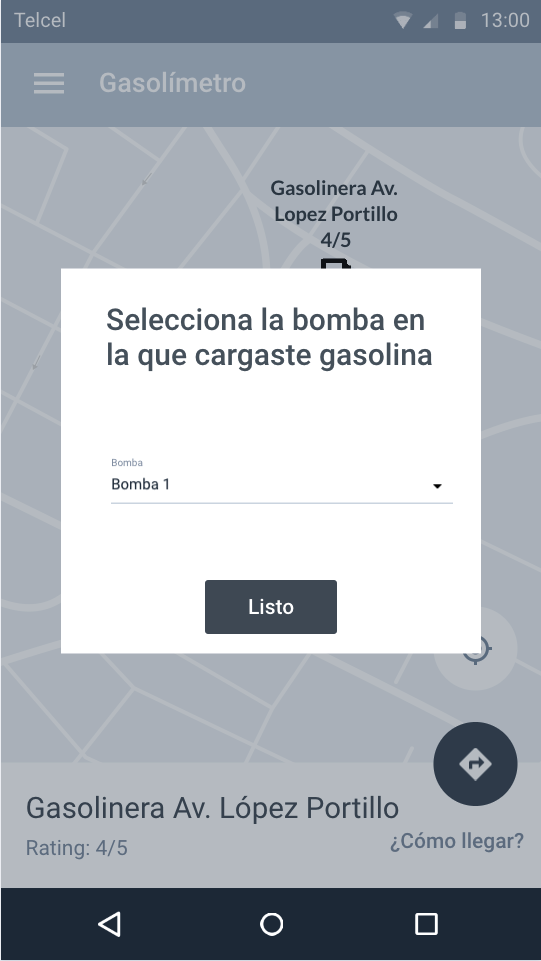
\includegraphics[scale=.55]{Capitulo4/software/submodulos/mediciones/images/sub-m-iu1_1_5_b}
	\caption{Interfaz de usuario SUB-M-IU1.1.5-Especificar bomba (b)}
	\label{fig:sub-m-iu1.1.5.b}
\end{figure}
%%%Usuarios
\subsubsection{SUB-U-IU1-Registrar usuario}\label{SUB-U-IU1}
\begin{figure}[H]
	\centering
	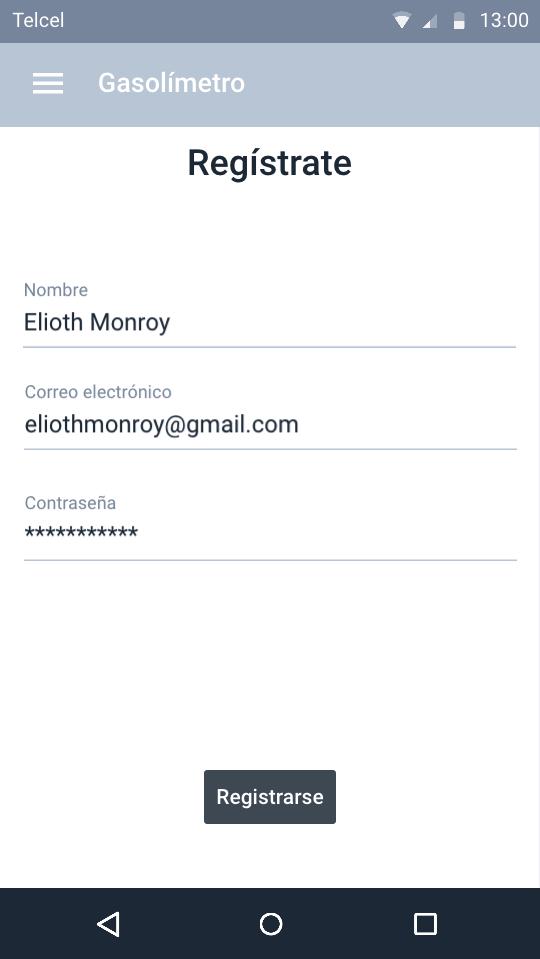
\includegraphics[scale=.55]{Capitulo4/software/submodulos/usuarios/images/sub-u-iu1}
	\caption{Interfaz de usuario SUB-U-IU1-Registrar usuario}
	\label{fig:sub-u-iu1}
\end{figure}
\subsubsection{SUB-U-IU1.1-Verificar cuenta}\label{SUB-U-IU1.1}
\begin{figure}[H]
	\centering
	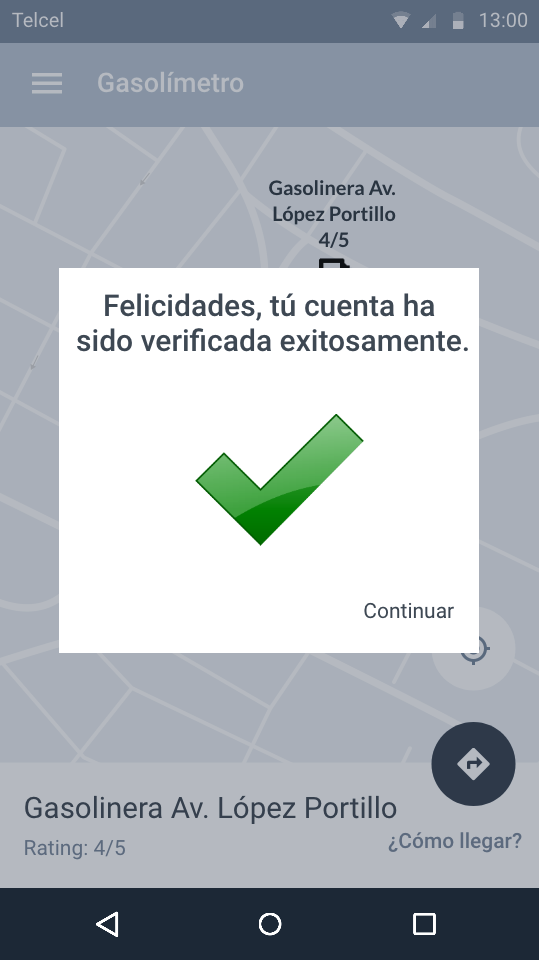
\includegraphics[scale=.55]{Capitulo4/software/submodulos/usuarios/images/sub-u-iu1_1}
	\caption{Interfaz de usuario SUB-U-IU1.1-Verificar cuenta}
	\label{fig:sub-u-iu1.1}
\end{figure}
\subsubsection{SUB-U-IU2-Editar usuario}\label{SUB-U-IU2}
\begin{figure}[H]
	\centering
	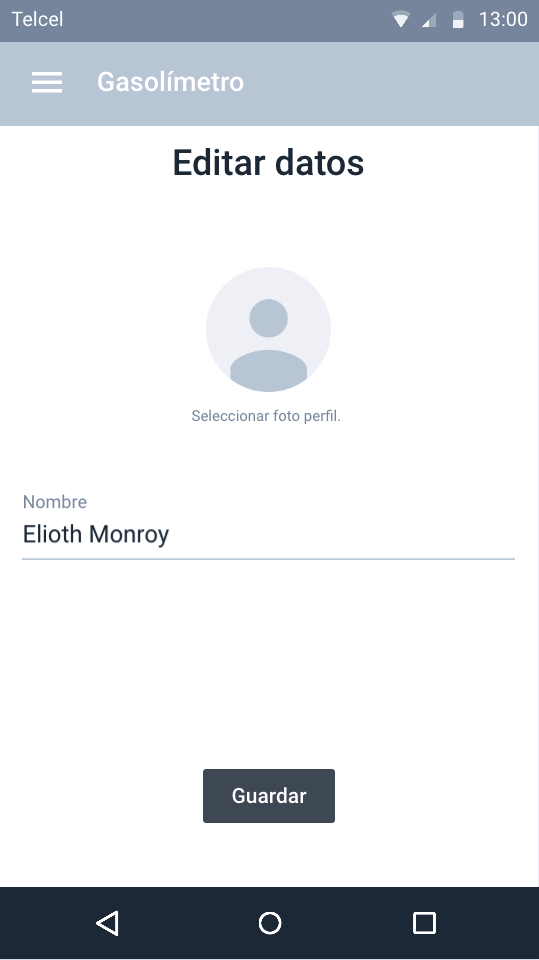
\includegraphics[scale=.55]{Capitulo4/software/submodulos/usuarios/images/sub-u-iu2}
	\caption{Interfaz de usuario SUB-U-IU2-Editar usuario}
	\label{fig:sub-u-iu2}
\end{figure}
\subsubsection{SUB-U-IU3-Consultar panel de control}\label{SUB-U-IU3}
\begin{figure}[H]
	\centering
	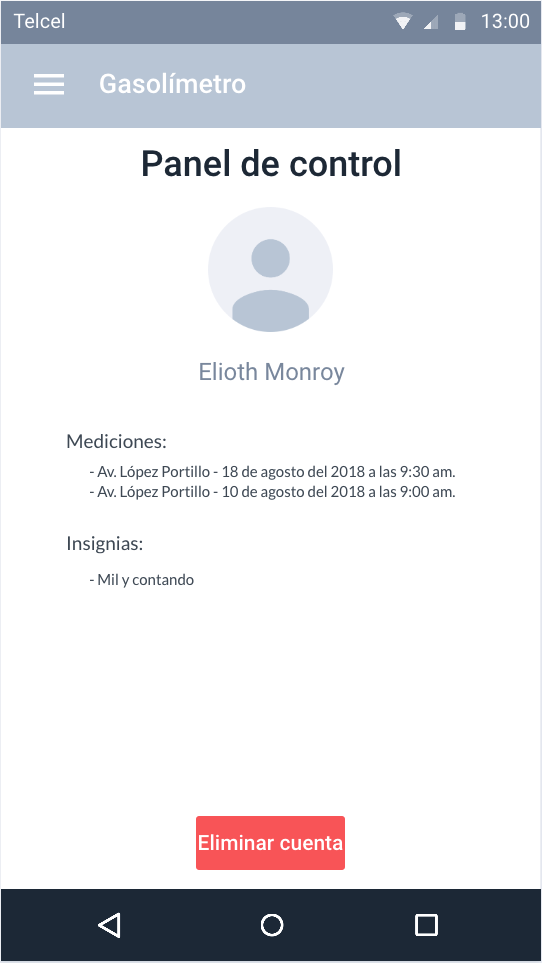
\includegraphics[scale=.55]{Capitulo4/software/submodulos/usuarios/images/sub-u-iu3}
	\caption{Interfaz de usuario SUB-U-IU3-Consultar panel de control}
	\label{fig:sub-u-iu3}
\end{figure}
\subsubsection{SUB-U-IU3.1-Consultar insignia}\label{SUB-C-IU3.1}
\begin{figure}[H]
	\centering
	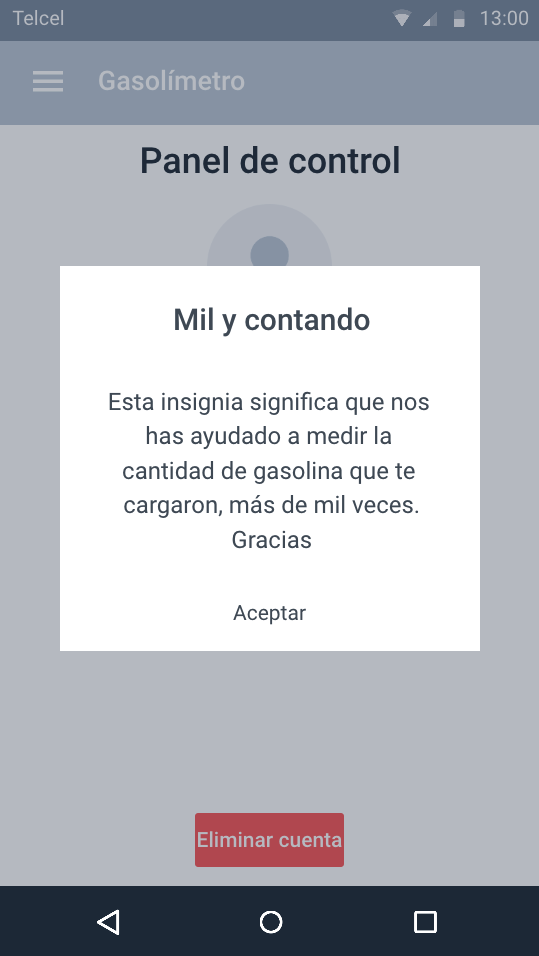
\includegraphics[scale=.55]{Capitulo4/software/submodulos/usuarios/images/sub-u-iu3_1}
	\caption{Interfaz de usuario SUB-U-IU3.1-Consultar insignia}
	\label{fig:sub-u-iu3.1}
\end{figure}
\subsubsection{SUB-U-IU4-Eliminar usuario}\label{SUB-U-IU1}
\begin{figure}[H]
	\centering
	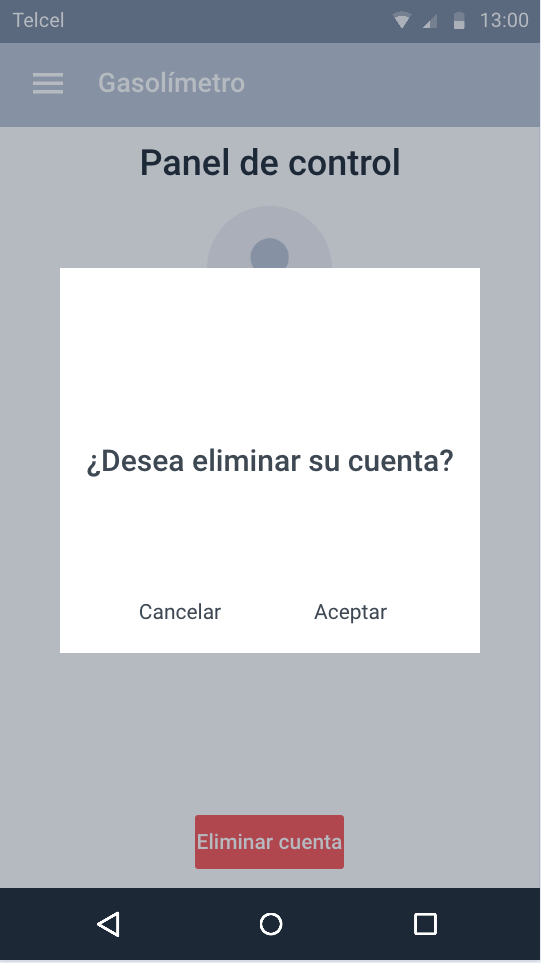
\includegraphics[scale=.55]{Capitulo4/software/submodulos/usuarios/images/sub-u-iu4}
	\caption{Interfaz de usuario SUB-U-IU4-Eliminar usuario}
	\label{fig:sub-u-iu4}
\end{figure}
\subsubsection{SUB-U-IU5-Autenticar usuario}\label{SUB-U-IU5}
\begin{figure}[H]
	\centering
	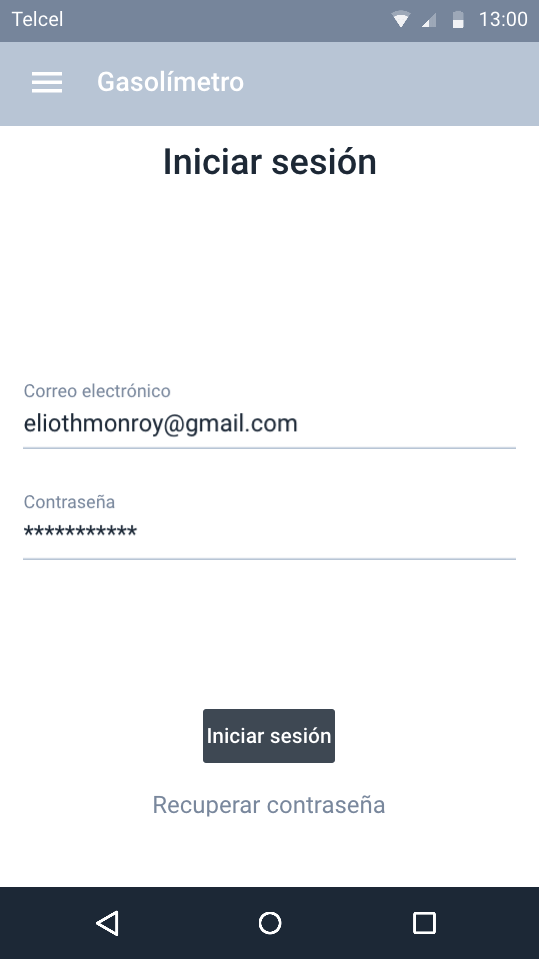
\includegraphics[scale=.55]{Capitulo4/software/submodulos/usuarios/images/sub-u-iu5}
	\caption{Interfaz de usuario SUB-U-IU5-Autenticar usuario}
	\label{fig:sub-u-iu5}
\end{figure}
\subsubsection{SUB-U-IU5.1-Autenticar usuario}\label{SUB-U-IU5.1}
\begin{figure}[H]
	\centering
	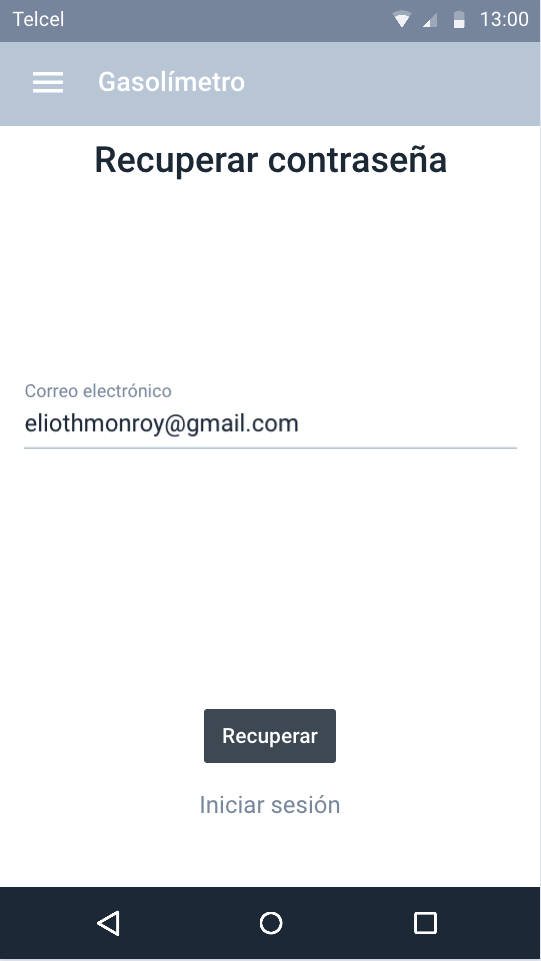
\includegraphics[scale=.55]{Capitulo4/software/submodulos/usuarios/images/sub-u-iu5_1}
	\caption{Interfaz de usuario SUB-U-IU5.1-Recuperar contraseña}
	\label{fig:sub-u-iu5.1}
\end{figure}
\subsubsection{SUB-U-IU6-Consultar medición}\label{SUB-C-IU6}
\begin{figure}[H]
	\centering
	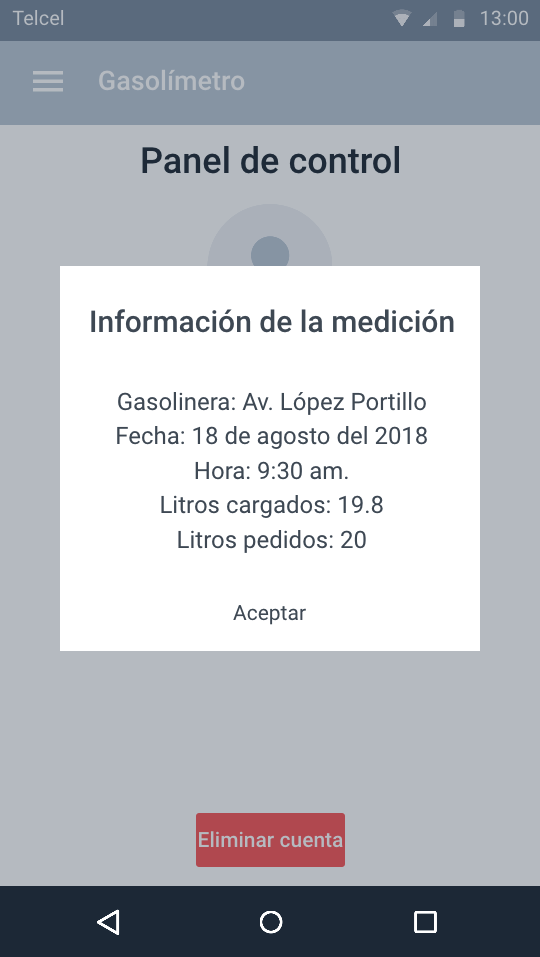
\includegraphics[scale=.55]{Capitulo4/software/submodulos/usuarios/images/sub-u-iu6}
	\caption{Interfaz de usuario SUB-U-IU6-Consultar medición}
	\label{fig:sub-u-iu6}
\end{figure}
\subsubsection{SUB-U-IU7-Compartir información}\label{SUB-U-IU7}
\begin{figure}[H]
	\centering
	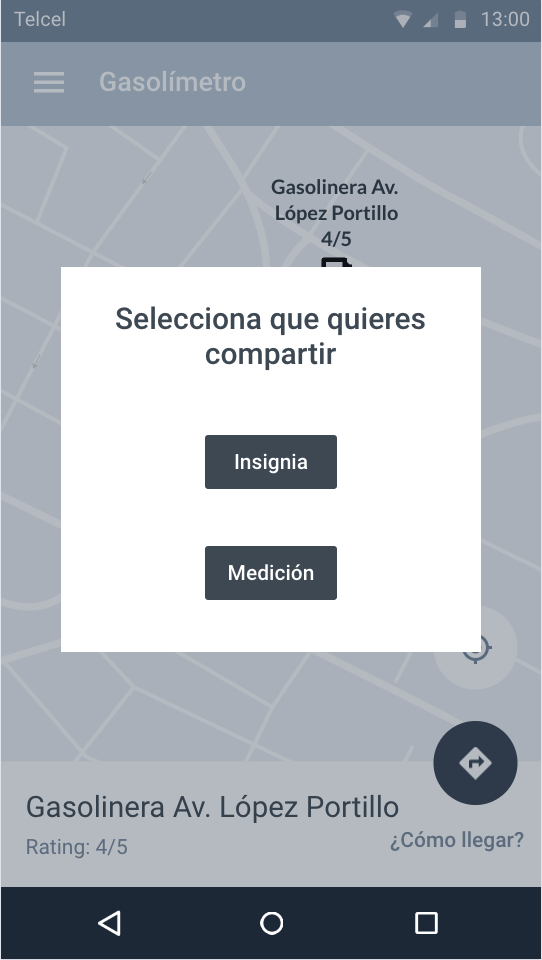
\includegraphics[scale=.55]{Capitulo4/software/submodulos/usuarios/images/sub-u-iu7_a}
	\caption{Interfaz de usuario SUB-U-IU7-Compartir información (a)}
	\label{fig:sub-u-iu7}
\end{figure}
\begin{figure}[H]
	\centering
	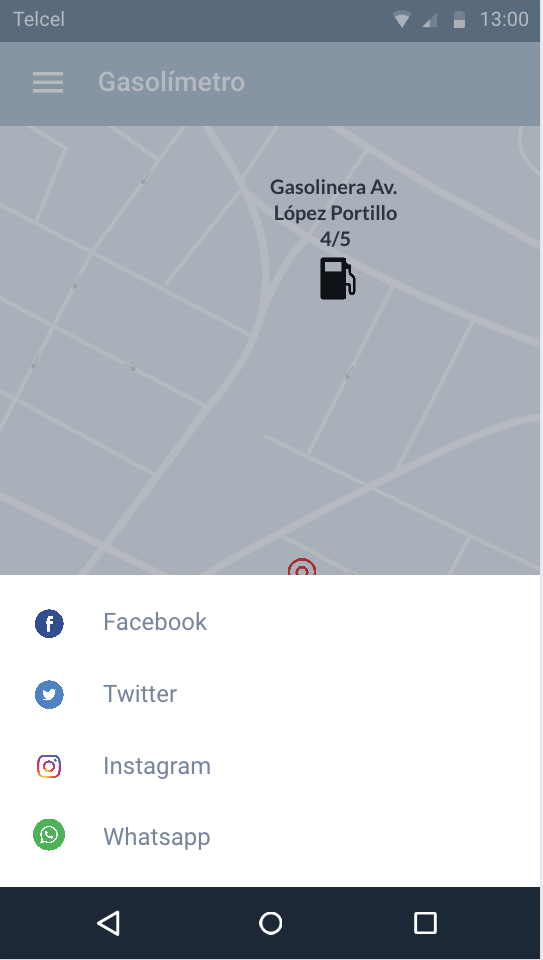
\includegraphics[scale=.55]{Capitulo4/software/submodulos/usuarios/images/sub-u-iu7_b}
	\caption{Interfaz de usuario SUB-U-IU7-Compartir información (b)}
	\label{fig:sub-u-iu7.b}
\end{figure}
\subsubsection{SUB-U-IU7.1-Compartir insignia}\label{SUB-U-IU7.1}
\begin{figure}[H]
	\centering
	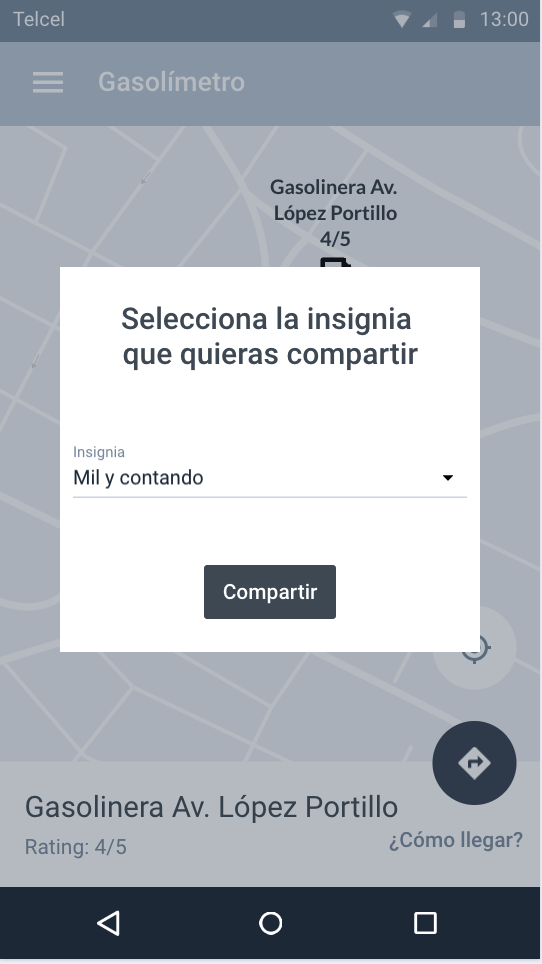
\includegraphics[scale=.55]{Capitulo4/software/submodulos/usuarios/images/sub-u-iu7_1}
	\caption{Interfaz de usuario SUB-U-IU7-Compartir insignia}
	\label{fig:sub-u-iu7}
\end{figure}
\subsubsection{SUB-U-IU8-Generar reporte}\label{SUB-U-IU8}
\begin{figure}[H]
	\centering
	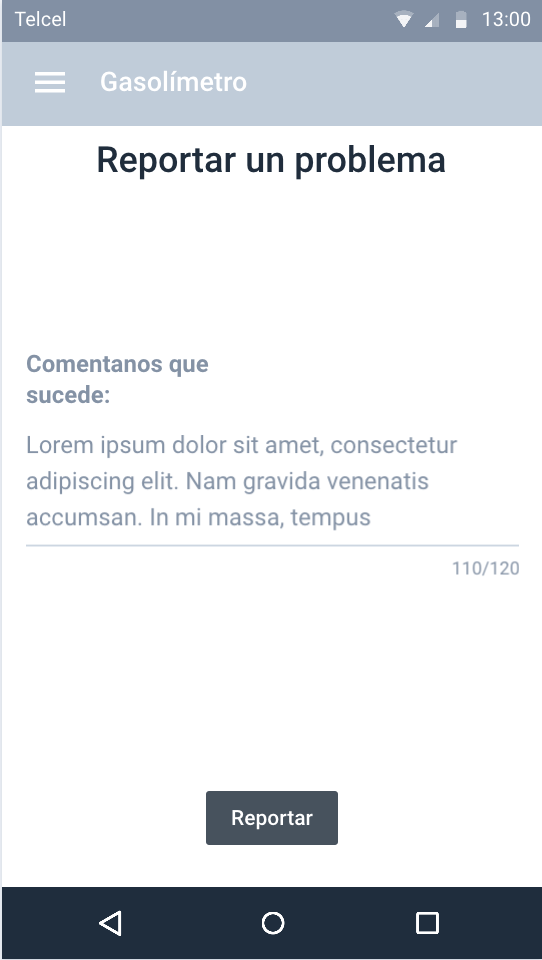
\includegraphics[scale=1]{Capitulo4/software/submodulos/usuarios/images/sub-u-iu8}
	\caption{Interfaz de usuario SUB-U-IU8-Generar reporte}
	\label{fig:sub-u-iu8}
\end{figure}
\subsubsection{SUB-U-IU9-Consultar reporte}\label{SUB-U-IU9}
\begin{figure}[H]
	\centering
	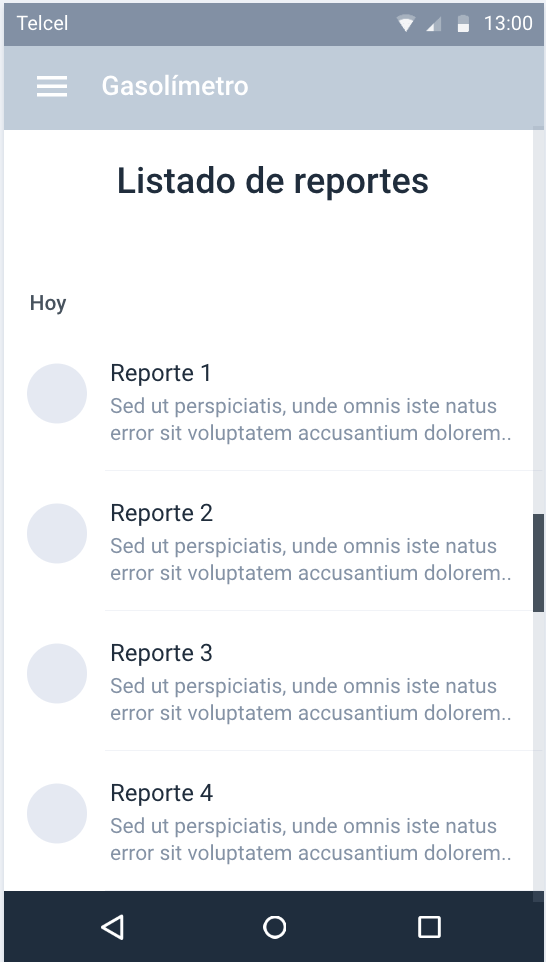
\includegraphics[scale=1]{Capitulo4/software/submodulos/usuarios/images/sub-u-iu9}
	\caption{Interfaz de usuario SUB-U-IU9-Consultar reporte}
	\label{fig:sub-u-iu9}
\end{figure}
\subsubsection{SUB-U-IU9.1-Generar reporte}\label{SUB-U-IU9.1}
\begin{figure}[H]
	\centering
	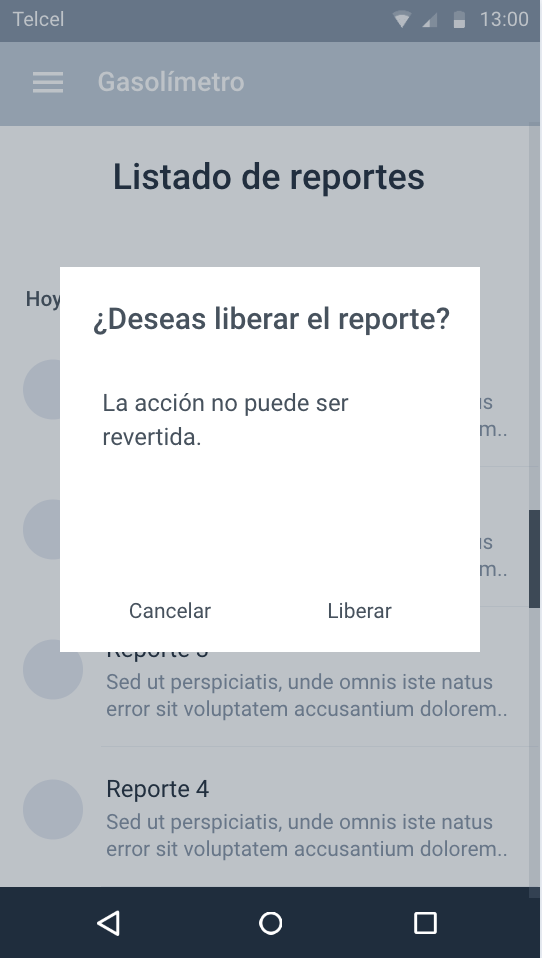
\includegraphics[scale=1]{Capitulo4/software/submodulos/usuarios/images/sub-u-iu9_1}
	\caption{Interfaz de usuario SUB-U-IU9.1-Consultar reporte}
	\label{fig:sub-u-iu9.1}
\end{figure}
\subsubsection{SUB-U-IU10-Registrar automóvil}\label{SUB-U-IU10}
\begin{figure}[H]
	\centering
	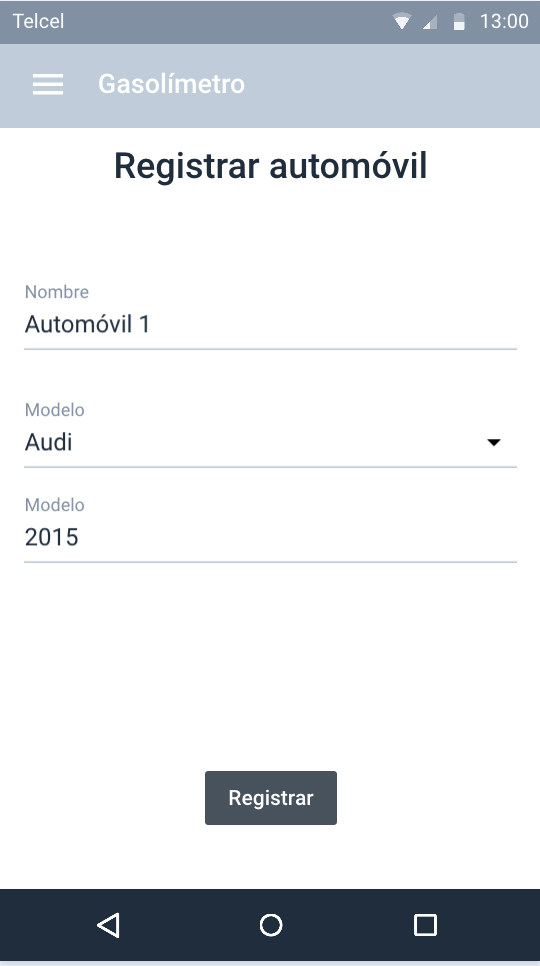
\includegraphics[scale=1]{Capitulo4/software/submodulos/usuarios/images/sub-u-iu10}
	\caption{Interfaz de usuario SUB-U-IU8-Registrar automóvil}
	\label{fig:sub-u-iu10}
\end{figure}
\subsubsection{SUB-U-IU11-Editar automóvil}\label{SUB-U-IU11}
\begin{figure}[H]
	\centering
	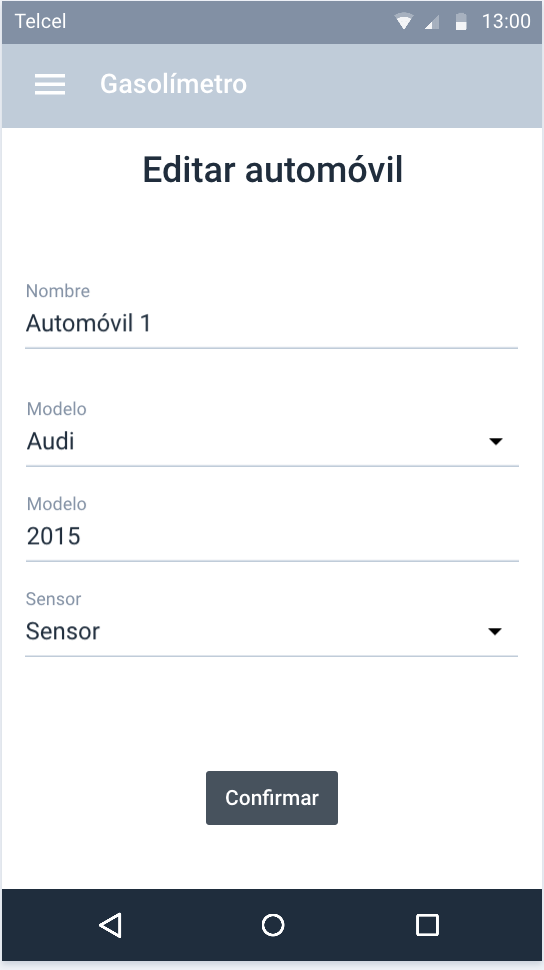
\includegraphics[scale=1]{Capitulo4/software/submodulos/usuarios/images/sub-u-iu11}
	\caption{Interfaz de usuario SUB-U-IU11-Editar automóvil}
	\label{fig:sub-u-iu11}
\end{figure}
\subsubsection{SUB-U-IU12-Consultar automóvil}\label{SUB-U-IU12}
\begin{figure}[H]
	\centering
	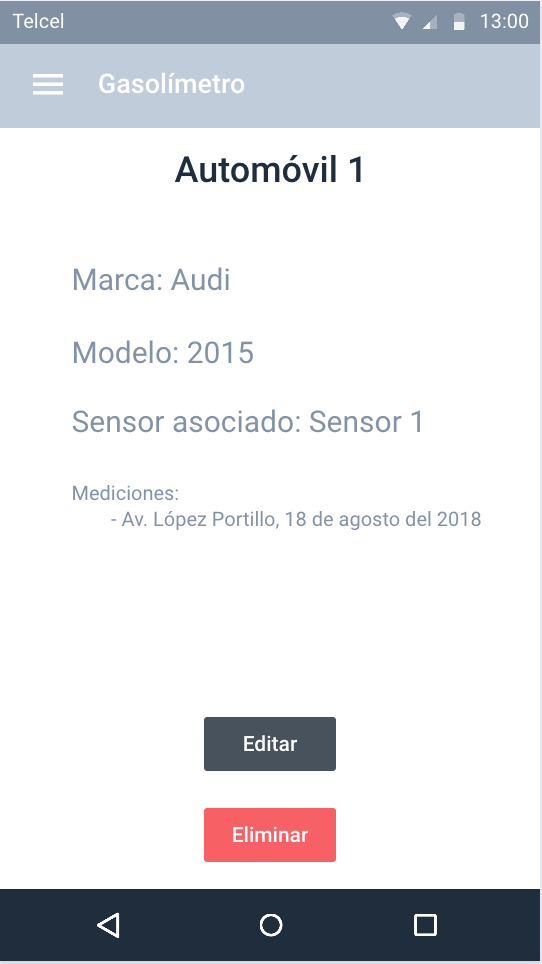
\includegraphics[scale=1]{Capitulo4/software/submodulos/usuarios/images/sub-u-iu12}
	\caption{Interfaz de usuario SUB-U-IU12-Consultar automóvil}
	\label{fig:sub-u-iu12}
\end{figure}
\subsubsection{SUB-U-IU13-Eliminar automóvil}\label{SUB-U-IU13}
\begin{figure}[H]
	\centering
	\includegraphics[scale=1]{Capitulo4/software/submodulos/usuarios/images/sub-u-iu13}
	\caption{Interfaz de usuario SUB-U-IU13-Eliminar automóvil}
	\label{fig:sub-u-iu13}
\end{figure}
\subsubsection{SUB-U-IU14-Registrar sensor}\label{SUB-U-IU14}
\begin{figure}[H]
	\centering
	\includegraphics[scale=1]{Capitulo4/software/submodulos/usuarios/images/sub-u-iu14}
	\caption{Interfaz de usuario SUB-U-IU14-Registrar sensor}
	\label{fig:sub-u-iu14}
\end{figure}
% \subsubsection{SUB-U-IU15-Eliminar sensor}\label{SUB-U-IU15}
\begin{figure}[H]
	\centering
	\includegraphics[scale=1]{Capitulo4/software/submodulos/usuarios/images/sub-u-iu15}
	\caption{Interfaz de usuario SUB-U-IU15-Eliminar sensor}
	\label{fig:sub-u-iu15}
\end{figure}
% \subsubsection{SUB-U-IU16-Asociar sensor-automóvil}\label{SUB-U-IU16}
\begin{figure}[H]
	\centering
	\includegraphics[scale=1]{Capitulo4/software/submodulos/usuarios/images/sub-u-iu16}
	\caption{Interfaz de usuario SUB-U-IU16-Asociar sensor-automóvil}
	\label{fig:sub-u-iu16}
\end{figure}
\subsubsection{SUB-U-IU17-Registrar gasolinera}\label{SUB-U-IU17}
\begin{figure}[H]
	\centering
	\includegraphics[scale=1]{Capitulo4/software/submodulos/usuarios/images/sub-u-iu17}
	\caption{Interfaz de usuario SUB-U-IU17-Registrar gasolinera}
	\label{fig:sub-u-iu17}
\end{figure}
\subsubsection{SUB-U-IU18-Consultar gasolinera}\label{SUB-U-IU18}
\begin{figure}[H]
	\centering
	\includegraphics[scale=1]{Capitulo4/software/submodulos/usuarios/images/sub-u-iu18}
	\caption{Interfaz de usuario SUB-U-IU18-Consultar gasolinera}
	\label{fig:sub-u-iu18}
\end{figure}
\subsubsection{SUB-U-IU19-Editar gasolinera}\label{SUB-U-IU19}
\begin{figure}[H]
	\centering
	\includegraphics[scale=1]{Capitulo4/software/submodulos/usuarios/images/sub-u-iu19}
	\caption{Interfaz de usuario SUB-U-IU19-Editar gasolinera}
	\label{fig:sub-u-iu19}
\end{figure}
\subsubsection{SUB-U-IU20-Eliminar gasolinera}\label{SUB-U-IU20}
\begin{figure}[H]
	\centering
	\includegraphics[scale=1]{Capitulo4/software/submodulos/usuarios/images/sub-u-iu20}
	\caption{Interfaz de usuario SUB-U-IU20-Eliminar gasolinera}
	\label{fig:sub-u-iu20}
\end{figure}
%%%Clasificación
\subsubsection{SUB-C-IU2-Consultar mapa}\label{SUB-C-IU2}
\begin{figure}[H]
	\centering
	\includegraphics[scale=.55]{Capitulo4/software/submodulos/clasificacion/images/sub-c-iu2}
	\caption{Interfaz de usuario SUB-C-IU2-Consultar mapa}
	\label{fig:sub-c-iu2}
\end{figure}
\subsubsection{SUB-C-IU2.1-Realizar recorrido}\label{SUB-C-IU2.1}
\begin{figure}[H]
	\centering
	\includegraphics[scale=.55]{Capitulo4/software/submodulos/clasificacion/images/sub-c-iu2_1}
	\caption{Interfaz de usuario SUB-C-IU2.1-Realizar recorrido}
	\label{fig:sub-c-iu2.1}
\end{figure}
\subsubsection{SUB-C-IU2.2-Consultar gasolinera}\label{SUB-C-IU2.2}
\begin{figure}[H]
	\centering
	\includegraphics[scale=.55]{Capitulo4/software/submodulos/clasificacion/images/sub-c-iu2_2}
	\caption{Interfaz de usuario SUB-C-IU2.2-Consultar gasolinera}
	\label{fig:sub-c-iu2.2}
\end{figure}